
%% LLT: Turn off some annoying warnings...
\RequirePackage{silence}
\WarningFilter{titlesec}{Non standard sectioning command}
\WarningFilter{scrreprt}{Usage of package}
\WarningFilter{scrreprt}{Activating an ugly workaround}

% **************************************************
% Document Class Definition
% **************************************************
\documentclass[%
	paper=A4,					
	twoside=true,				
	openright,					% doublepage cleaning ends up right side
	parskip=full,				% spacing value / method for paragraphs
	chapterprefix=true,			% prefix for chapter marks
	12pt,						% font size
	headings=normal,			% size of headings
	bibliography=totoc,			% include bib in toc
	listof=totoc,				% include listof entries in toc
	titlepage=on,				% own page for each title page
	captions=tableabove,		% display table captions above the float env
	draft=false,				% value for draft version
]{scrreprt}%

% **************************************************
% Debug LaTeX Information
% **************************************************
%\listfiles

% **************************************************
% Information and Commands for Reuse
% **************************************************
\newcommand{\thesisTitle}{Searches for Astrophysical Neutrino Sources: from Gigaelectronvolt to Exaelectronvolt}
\newcommand{\thesisName}{Alex Pizzuto}
\newcommand{\thesisSubject}{Particle Astrophysics}
\newcommand{\thesisDate}{\today}
\newcommand{\thesisVersion}{1.1}

\newcommand{\thesisFirstReviewer}{Reviewer 1}
\newcommand{\thesisFirstReviewerUniversity}{\protect{University of Wisconsin - Madison}}
\newcommand{\thesisFirstReviewerDepartment}{Department of Physics}

\newcommand{\thesisSecondReviewer}{Reviewer 2}
\newcommand{\thesisSecondReviewerUniversity}{\protect{University of Wisconsin - Madison}}
\newcommand{\thesisSecondReviewerDepartment}{Department of Physics}

\newcommand{\thesisFirstSupervisor}{Justin Vandenbroucke}

\newcommand{\thesisUniversity}{\protect{University of Wisconsin - Madison}}
\newcommand{\thesisUniversityDepartment}{Department of Physics}
\newcommand{\thesisUniversityInstitute}{Wisconsin IceCube Particle Astrophysics Center}
\newcommand{\thesisUniversityGroup}{IceCube Neutrino Observatory: Neutrino Sources WG}
\newcommand{\thesisUniversityCity}{Madison, WI}
\newcommand{\thesisUniversityStreetAddress}{222 W Washington Ave UNIT 500}
\newcommand{\thesisUniversityPostalCode}{53703}

% **************************************************
% Load and Configure Packages
% **************************************************
\usepackage[utf8]{inputenc}		% defines file's character encoding
\usepackage[english]{babel} % babel system, adjust the language of the content
\usepackage[					% clean thesis style
	figuresep=colon,%
	sansserif=false,%
	hangfigurecaption=false,%
	hangsection=true,%
	hangsubsection=true,%
	colorize=full,%
	colortheme=bluemagenta,%
% LLT: Use biber if using UTF8 encoding
% 	bibsys=bibtex,%
	bibsys=biber,%
	bibfile=bib-refs,%
	bibstyle=alphabetic,%
]{cleanthesis}

\usepackage{amsmath,amstext}
\usepackage{amsfonts}
\usepackage{pdfpages}
\usepackage[T1]{fontenc}
%\usepackage{apjfonts} 
%\usepackage[figure,figure*]{hypcap}
\usepackage[utf8]{inputenc}
\usepackage{array}
\usepackage{makecell}
\usepackage{booktabs}
\usepackage{threeparttable}
\usepackage{mathrsfs}
\usepackage{mathtools}
%\usepackage{lineno}
\usepackage{footmisc}
\usepackage{multirow}
\newcommand*\diff{\mathop{}\!\mathrm{d}}
\newcommand*\numu{$\nu_{\mu}$ }
\newcommand*\nutau{$\nu_{\tau}$ }
\newcommand*\nue{$\nu_{e}$ }
\newcommand*\numubar{$\bar{\nu}_{\mu}$ }
\newcommand*\nutaubar{$\bar{\nu}_{\tau}$ }
\newcommand*\nuebar{$\bar{\nu}_{e}$ }

\hypersetup{					% setup the hyperref-package options
	pdftitle={\thesisTitle},	% 	- title (PDF meta)
	pdfsubject={\thesisSubject},% 	- subject (PDF meta)
	pdfauthor={\thesisName},	% 	- author (PDF meta)
	plainpages=false,			% 	-
	colorlinks=false,			% 	- colorize links?
	pdfborder={0 0 0},			% 	-
	breaklinks=true,			% 	- allow line break inside links
	bookmarksnumbered=true,		%
	bookmarksopen=true			%
}
\usepackage{tikz} 
\usetikzlibrary{shapes,arrows,positioning,automata,backgrounds,calc,er,patterns}
\usepackage{tikz-feynman}
\tikzfeynmanset{every vertex/.style={red, dot},
every particle/.style={blue},
every blob/.style={draw=green!40!black, pattern color=green!40!black}
}
\usepackage{listings}
% \usepackage{subcaption}
% \captionsetup{compatibility=false}
\usepackage{graphicx,subfigure}


% **************************************************
% Document CONTENT
% **************************************************
\begin{document}

\newcommand\brabar{\scalebox{.3}{(}\raisebox{-1.7pt}{$-$}\scalebox{.3}{)}}

% --------------------------
% rename document parts
% --------------------------
\renewcaptionname{english}{\figurename}{Fig.}
\renewcaptionname{english}{\tablename}{Tab.}

% --------------------------
% Front matter
% --------------------------
\pagenumbering{roman}			% roman page numbing (invisible for empty page style)
\pagestyle{empty}				% no header or footers
% !TEX root = ../thesis-example.tex
%
% ------------------------------------  --> cover title page
\begin{titlepage}
	\pdfbookmark[0]{Cover}{Cover}
	\flushright
	\hfill
	\vfill
	{\LARGE\thesisTitle \par}
	\rule[5pt]{\textwidth}{.4pt} \par
	{\Large\thesisName}
	\vfill
	\textit{\large\thesisDate} \\
	Version: \thesisVersion
\end{titlepage}


% ------------------------------------  --> main title page
\begin{titlepage}
	\pdfbookmark[0]{Titlepage}{Titlepage}
	\tgherosfont
	\centering

	{\Large \thesisUniversity} \\[4mm]
	
\includegraphics[width=5cm]{gfx/WIPAC_logo.png}  
\includegraphics[width=6cm,trim={0cm 1cm 0cm 1cm}]{gfx/UW_logo.png}\\[2mm]
	\textsf{\thesisUniversityDepartment} \\
	\textsf{\thesisUniversityInstitute} \\
	%\textsf{\thesisUniversityGroup} \\

	\vfill
	%{\large \thesisSubject} \\[5mm]
	{\LARGE \color{ctcolortitle}\textbf{\thesisTitle} \\[10mm]}
	{\Large \thesisName} \\

	\vfill
	\begin{minipage}[t]{.27\textwidth}
		\raggedleft
		\textit{1. Reviewer}
	\end{minipage}
	\hspace*{15pt}
	\begin{minipage}[t]{.65\textwidth}
		{\Large \thesisFirstReviewer} \\
	  	{\small \thesisFirstReviewerDepartment} \\[-1mm]
		{\small \thesisFirstReviewerUniversity}
	\end{minipage} \\[5mm]
	\begin{minipage}[t]{.27\textwidth}
		\raggedleft
		\textit{2. Reviewer}
	\end{minipage}
	\hspace*{15pt}
	\begin{minipage}[t]{.65\textwidth}
		{\Large \thesisSecondReviewer} \\
	  	{\small \thesisSecondReviewerDepartment} \\[-1mm]
		{\small \thesisSecondReviewerUniversity}
	\end{minipage} \\[10mm]
	\begin{minipage}[t]{.27\textwidth}
		\raggedleft
		\textit{Supervisor:}
	\end{minipage}
	\hspace*{15pt}
	\begin{minipage}[t]{.65\textwidth}
		\thesisFirstSupervisor\ 
	\end{minipage} \\[10mm]

	\thesisDate \\

\end{titlepage}


% ------------------------------------  --> lower title back for single page layout
\hfill
\vfill
{
	\small
	\textbf{\thesisName} \\
	\textit{\thesisTitle} \\
	\thesisSubject, \thesisDate \\
	Reviewers: \thesisFirstReviewer\ and \thesisSecondReviewer \\
	Supervisor: \thesisFirstSupervisor \\[1.5em]
	\textbf{\thesisUniversity} \\
	\textit{\thesisUniversityGroup} \\
	\thesisUniversityInstitute \\
	\thesisUniversityDepartment \\
	\thesisUniversityStreetAddress \\
	\thesisUniversityPostalCode\  \thesisUniversityCity
}
		% INCLUDE: all titlepages
\clearpage

\pagestyle{plain}				% display just page numbers
% !TEX root = ../thesis-example.tex
%
\pdfbookmark[0]{Abstract}{Abstract}
\chapter*{Abstract}
\label{sec:abstract}
\vspace*{-10mm}

Abstract goes here

\vspace*{20mm}

		% INCLUDE: the abstracts 
\clearpage
%
% !TEX root = ../thesis-example.tex
%
\pdfbookmark[0]{Acknowledgement}{Acknowledgement}
\chapter*{Acknowledgement}
\label{sec:acknowledgement}
\vspace*{-10mm}

Acknowledgements go here
 % INCLUDE: acknowledgement
\clearpage
%
\setcounter{tocdepth}{2}		% define depth of toc
\tableofcontents				% display table of contents
\clearpage

% --------------------------
% Body matter
% --------------------------
\pagenumbering{arabic}			% arabic page numbering
\setcounter{page}{1}			% set page counter
\pagestyle{maincontentstyle} 	% fancy header and footer

\part{Searching for Astrophysical Neutrino Sources}
% !TEX root = ../thesis-example.tex
%
\chapter{Introduction}
\label{sec:intro}

\cleanchapterquote{The energy in the extreme Universe in photons and neutrinos is the same}{Francis Halzen}{(ICRC 2019)}


\section{Multi-Messenger Astronomy}
\label{sec:intro:multimessenger}



\subsection{Photons and gamma rays}
\label{sec:intro:gammarays}


\subsection{Cosmic rays}
\label{sec:intro:cosmicrays}


\textbf{Chapter \ref{sec:neutrinos}} \\[0.2em]

\textbf{Chapter \ref{sec:intro}} \\[0.2em]

 
\chapter{Neutrinos}
\label{sec:neutrinos}

\cleanchapterquote{Decide on a quote to put here}{quote person}{(quote person job)}


\section{Neutrinos}
\label{sec:intro:multimessenger}



\section{Neutrino Detection}
\label{sec:intro:gammarays}



\subsection{Cherenkov Radiation}
\label{sec:intro:cosmicrays}
 
\chapter{The IceCube Neutrino Observatory}
\label{sec:IceCube}

\cleanchapterquote{It's morphology, not topology}{Justin Vandenbroucke}{(University of Wisconsin-Madison)}


\section{The IceCube Detector}
\label{sec:intro:detector}




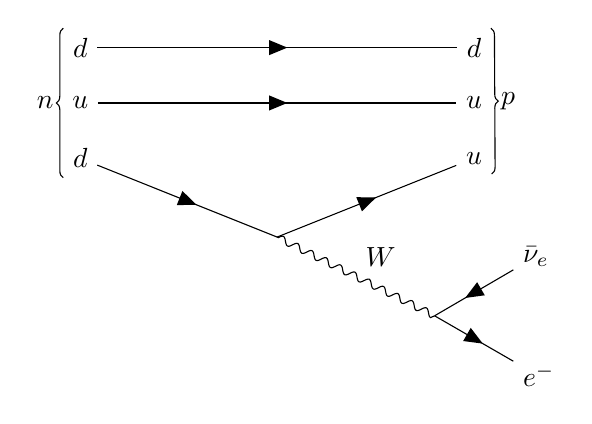
\begin{tikzpicture}
\begin{feynman}
\vertex (d1) {\(d\)}; 
\vertex[right=5cm of d1] (d2) {\(d\)}; 
\vertex[below=2em of d1] (u1) {\(u\)}; 
\vertex[right=5cm of u1] (u2) {\(u\)};
\vertex[below=2em of u1] (d3) {\(d\)}; 
\vertex[right=5cm of d3] (u3) {\(u\)};
\vertex[below right=1cm and 2.5cm of d3] (v1);
\vertex[below right=1cm and 2cm of v1] (v2);
\vertex[above right=0.5cm and 1cm of v2] (nu) {$\bar\nu_e$};
\vertex[below right=0.5cm and 1cm of v2] (e) {$e^-$};
\diagram* { {[edges=fermion]
(d1) -- (d2),  (u1) -- (u2),
(d3) -- (v1) -- (u3), (nu) -- (v2) -- (e)},
(v1) -- [boson, edge label=\(W\)] (v2)
};
\draw [decoration={brace}, decorate] (d3.south west) -- (d1.north west) node [pos=0.5, left] {\(n\)};
\draw [decoration={brace}, decorate] (d2.north east) --  (u3.south east) node [pos=0.5, right] {\(p\)};
\end{feynman} 
\end{tikzpicture}



\section{Reconstruction Algorithms}
\label{sec:intro:reconstruction}



\section{Event Selections}
\label{sec:icecube:eventselection}



\section{Astrophysical Neutrino Flux}
\label{sec:intro:astroflux}


\chapter{Analysis Methods}
\label{sec:nusources}

\cleanchapterquote{Decide on a quote to put here}{quote person}{(quote person job)}


\section{Maximum Likelihood Methodology}
\label{sec:nusources:lieklihood}


\subsection{Test Statistic}
\label{sec:nusources:TS}


\subsection{Transient Analyses}
\label{sec:nusources:transient}

\subsection{Steady Sources}
\label{sec:nusources:steady}

\subsection{Single Flare Analyses}
\label{sec:nusources:flare}

\section{Sensitivity and Discovery Potential}
\label{sec:sensitivity}


\section{Features of transient analyses}
\label{sec:transient_dip}



\chapter{Search for GeV Neutrinos from Galactic Novae}
\label{sec:Novae}

\cleanchapterquote{Decide on a quote to put here}{quote person}{(quote person job)}


\section{Models}
\label{sec:Novae:models}


\section{Analysis description}
\label{sec:Novae:analysis}
\chapter{Fast Response Analysis}
\label{sec:FRA}
\chapter{Multi-wavelength neutrino astronomy and EeV neutrino source searches}
\label{sec:ANITA}


The \textbf{AN}tarctic \textbf{I}mpulsive \textbf{T}ransient \textbf{A}ntenna (ANITA) is yet another experiment that searches for neutrino interactions that take place in the Antarctic ice. Throughout the experiment's first three flights, the ANITA collaboration has detected 2 anomalous events that are potential neutrino candidates as well as a candidate event from another detection channel. This chapter describes the followup we performed to search for possible astrophysical origins of these events, and outlines the limits we are able to set connecting a non-observation in the TeV - PeV range to the claimed observations in the EeV regime.


\section{Cosmogenic Neutrinos}
\label{sec:ANITA:cosmogenic}
As described in section XXX, at the highest energies, the Universe is opaque to photons, as they interact with CMB photons between their inception and arrival on Earth. A similar process occurs with UHECRs, albeit at much higher energies, due to the $\Delta^{+}$ resonance, 
\begin{equation}
    \label{eq:delta_cmb}
    p+\gamma_{\text{C M B}} \rightarrow \Delta^{+} \rightarrow n(p)+\pi^{+}\left(\pi^{0}\right) \; .
\end{equation}
The temperature of CMB photons ($\approx$ 2.7 K) fixes the proton energy for this resonance to be at or above around $10^{19.5}$ EeV. This resonant cross section leads to a steepening of the cosmic-ray spectrum, predicted independently by Griesen \cite{Greisen:1966jv} as well as Zatsepin and Kuzmin \cite{Zatsepin:1966jv} (this cutoff eponymously takes the name the ``GZK cutoff''). 

While this process limits the reach of UHECR protons to be within a few tens of Mpc from their production sites, the mesonic products of this cutoff lead to an increase in the UHE neutrino flux (``GZK'' or ``cosmogenic'' neutrinos) \cite{Beresinsky:1969qj}. Just as with the $pp$ and $p\gamma$ interactions discussed in Section XXX, the charged pions created from the UHECR-CMB interactions will decay into neutrinos, each of which carries a few percent of the initial UHE proton energy. 

However, by considering the magnitude of the predicted neutrino fluxes from bottom-up models with AGN \cite{Murase:2015ndr, Murase:2014foa}, pulsars \cite{Fang:2013vla}, low-luminosity GRBs \cite{Boncioli:2018lrv}, Tidal Disruption Events \cite{Biehl:2017hnb}, or binary neutron stars \cite{Fang:2017tla}, or by considering the remaining parameter space from current experimental constraints \cite{Kotera:2010yn, Ahlers:2010fw, Ahlers:2012rz, Heinze:2019jou}, it quickly becomes clear that instrumented volumes exceeding that of a cubic-kilometer are necessary to detect the GZK neutrino flux. 

One way to circumvent this problem is to, instead of searching for blue-ultraviolet wavelength photons from Cherenkov radiation, search for coherent radio emission. In the 1960's, Gurgen Askaryan noted that if an electromagnatic (EM) shower develops in a dielectric such as ice, then preferential annihilation of positrons leads to an overall negative charge excess \cite{Askaryan:1962hbi}. This $\sim$20\% negative charge excess gives rise to coherent Cherenkov radiation at long wavelenghts (and destructive interference for wavelengths comparable to the transverse shower size), named Askaryan radiation. In ice, this effect is coherent out to a few GHz \cite{Gorham:2006fy}.

Additionally, cosmic rays that enter the atmosphere with energies around $10^{15}$ eV can form particle cascades, known as extensive air showers (EAS). The observable radiation from EAS is in part due to Askaryan radiation \cite{Aab:2014esa}, though the dominant contribution is from geomagnetic radiation \cite{Kahn:1966}, in which the electrons and positrons in EAS are split by, and oscillate around, the Earth's magnetic field. 



\section{The ANITA Experiment}
\label{sec:ANITA:detector}
The ANtarctic Impulsive Transient Antenna (ANITA) is a NASA long duration balloon designed to detect radiation from UHE neutrinos interactions and EAS. At the time of writing, ANITA had flown four successful flights, with published results from the first three flights. A schematic of the detector as well as its various detection channels are displayed in Figure~\ref{fig:ANITA_instrument}. 

\begin{figure}
\centering
\subfigure{\label{fig:ANITA_cartoon}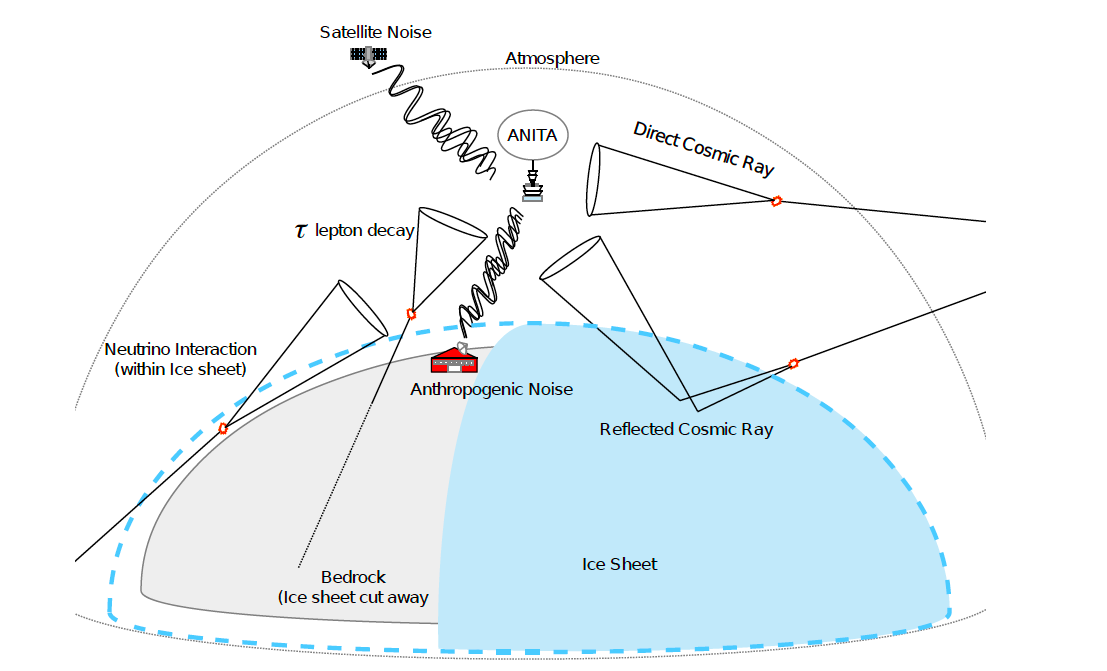
\includegraphics[width=.65\linewidth]{figures/ANITA/ANITA_signals.png}}
\subfigure{\label{fig:ANITA_detector}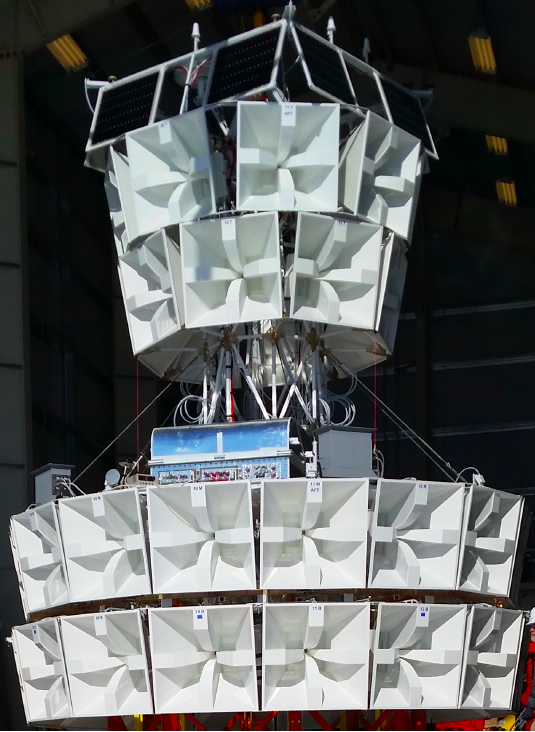
\includegraphics[width=.3\linewidth]{figures/ANITA/ANITA_detector.png}}
\caption[ANITA detector schematic]{(left) Sources to which ANITA is sensitive, with the exception of thermal noise. (right) The ANITA payload before the instrument's fourth flight. Both images taken from \cite{Ludwig:2019}.}
\label{fig:ANITA_instrument}
\end{figure}

In the search for the UHE component of the diffuse neutrino flux, ANITA has set the most constraining upper limits between $10^{19.5}$ and $10^{21}$ eV, combining results from the experiment's first three flights \cite{Gorham:2008yk, Gorham:2010kv, Allison:2018cxu}. However, in some of these analyses, individual candidate events were detected. Although these events were consistent with background estimates, one candidate event in ANITA-III was noted to have signal shape consistent with impulsive broadband emission that is characteristic of neutrino origin and to have originated from a location on the continent consistent with simulated distribution of neutrinos \cite{Allison:2018cxu}, although the detection of one candidate event is consistent with the background estimates of $0.7^{+0.5}_{-0.3}$ for these analyses. Private conversation with a member of the collaboration highlighted the event as an interesting candidate. 

Although the diffuse neutrino flux has been the instrument's main science goal, the first flights have resulted in a few enigmatic detections. ANITA also reported two additional events, each consistent with a an astrophysical $\nu_{\tau}$ emerging from the Earth \citep{Feng:2001ue, Gorham:2016zah, Gorham:2018ydl}. In this scenario, a $\nu_{\tau}$ undergoes a charged-current interaction (CC) with a nucleus in the Earth. The $\tau$-lepton produced in this interaction subsequently decays in the atmosphere, producing an extensive air shower (EAS). The polarity of the radio signal allows one to identify and reject downward moving cosmic-ray induced EAS, as the radio signals of these EAS acquire a phase reversal (opposite polarity) from reflection off the Antarctic ice, while an upgoing $\tau$ induced EAS does acquire this phase reversal. The schematic in figure \ref{fig:ANITA_instrument} highlights the distinction between the types of signals to which ANITA is sensitive. 

However, this interpretation poses many challenges  under Standard Model assumptions. First, for the observation angles and implied energies of the ANITA events, neutrinos are extremely unlikely to traverse the required chord lengths \citep{Gorham:2016zah}, even after accounting for an increase in the probability due to $\nu_{\tau}$ regeneration (explained in more detail later in this chapter). Second, if these events are of cosmogenic origin, they would imply fluxes that are in severe tension with limits set by multiple experiments \citep{Aab:2015kma, Zas:2017xdj, Aartsen:2016ngq} as well as a self-inconsistency from ANITA data alone. For an incident isotropic flux of neutrinos, for every one event arriving at elevation angles similar to the anomalous ANITA events (AAE), many events would be expected at other elevation angles, due to the detector's observation-angle dependent differential acceptance \citep{Romero-Wolf:2018zxt}.

\section{Followup Motivation}
\label{sec:ANITA_followup}
If the ANITA events are considered to have originated from individual cosmic accelerators, then there is no inconsistency with diffuse extremely-high-energy flux limits. This is especially true for accelerators with short characteristic timescales of emission, as many current limits on neutrino point-sources are for integrated emission over various experiments' livetimes \citep{Aartsen:2018ywr} and also as the acceptance of ANITA to a specific location on the sky changes throughout the detector's flight. Therefore, if ANITA detects a single event with an energy above 1 EeV from an incident $E^{-\gamma}$ power law flux, then there should also a large flux of neutrinos with TeV - PeV energies, to which neutrino telescopes such as IceCube would be sensitive. Significant correlation between IceCube and ANITA data would not only lend evidence for a neutrino point source, but it would also eliminate non-astrophysical explanations of the AAE, such as background and systematics or non-astrophysical models which invoke physics beyond the Standard Model.

In the following sections, we outline a followup performed to test the hypothesis that the ANITA neutrino candidate events were astrophysical in origin. We followup the 2 AAE as well as the one AAC. 

\section{Analysis description}
\label{sec:ANITA:analysis}

The likelihood analysis procedure described in Section~\ref{sec:nusources:lieklihood} describes how to search for a point source from a well localized direction. However, the events which ANITA detects have uncertainties comparable, if not larger than, events which IceCube detects, with localizations on the reconstructed shower coordinates on the order of a few degrees for 39\% containment. Here, we outline the differences between this analysis and the generic point source analyses described in the previous chapter, and we do not go into detail on the PDFs in the likelihood that are generated in manners similar to those presented in Section~\ref{sec:nusources:lieklihood}. 

In order to incorporate this uncertainty into our analysis, we employ a joint likelihood,

\begin{equation}
\label{eq:joint_likelihood}
     \mathcal{L} = \lambda \prod_{i=1}^{N} \Bigg( \frac{n_s}{n_s + n_b}S(\mathbf{x}_i, \mathbf{x}_s)  + \frac{n_b}{n_s + n_b}B(\mathbf{x}_i, \mathbf{x}_s) \Bigg) P_A(\mathbf{x}_s) \; .
\end{equation}
This likelihood is identical to that of section \ref{sec:nusources:lieklihood}, with the exception of one additional multiplicative term, $P_A(\mathbf{x}_s)$, which describes the ANITA event localization PDFs. Instead of calculating a TS from maximizing the likelihood at a fixed location on the sky, the TS is calculated at \textit{all} locations on the sky. At each location on the sky, $\mathbf{x}_s$, the usual TS is modified as a result of the ANITA prior, and the overall TS becomes

\begin{equation}
    \label{eq:TS_spatial_prior}
    \text{TS} = \max_{\mathbf{x}_s} \Bigg( \sum_{i=1}^{N}2\log \left[ 1 + \frac{\hat{n_s} S(\mathbf{x}_i, \mathbf{x}_s)}{n_b B(\mathbf{x}_i)} \right] + 2 \log \left[ \frac{P_A (\mathbf{x}_s)}{P_A (\mathbf{x}_0)} \right] \Bigg)\; .
\end{equation}

\begin{figure}
\centering
\begin{subfigure}
  \centering
  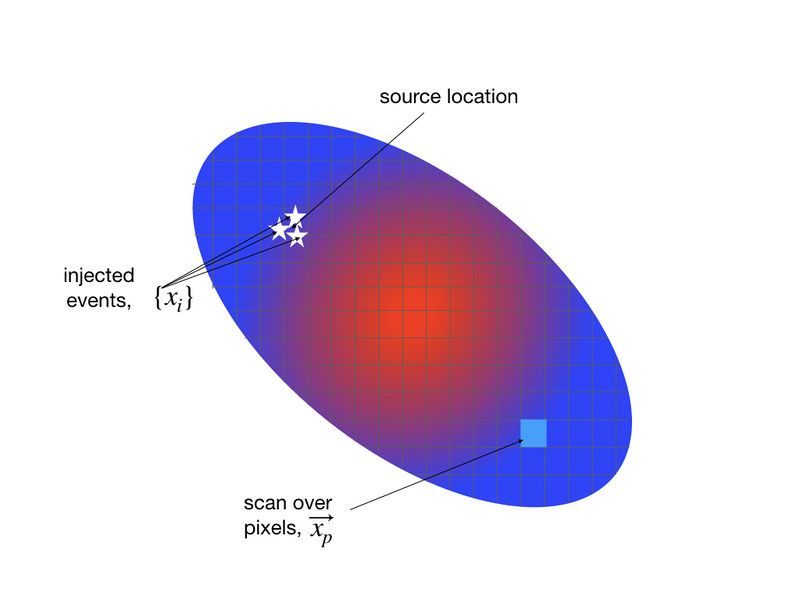
\includegraphics[width=.48\linewidth]{figures/ANITA/PixelScan_ANITA.jpeg}
  %\caption{A subfigure}
  %\label{fig:ANITA_cartoon}
\end{subfigure}%
\begin{subfigure}
  \centering
  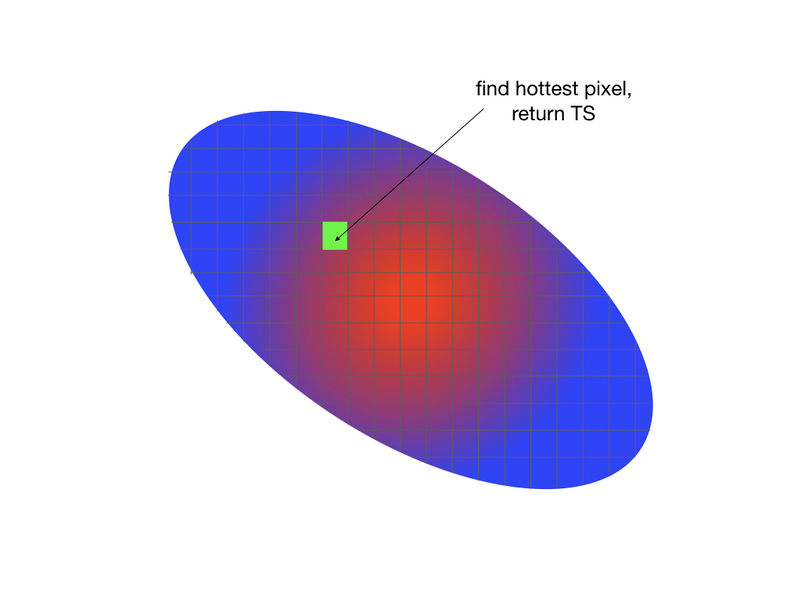
\includegraphics[width=.48\linewidth]{figures/ANITA/Hotspot_ANITA.jpeg}
  %\caption{A subfigure}
  %\label{fig:ANITA_detector}
\end{subfigure}
\caption[Spatial prior schematic]{Consider a neutrino source as depicted in the diagram on the left. The source's PDF from another experiment (such as ANITA) is given by the ellipsoidal colored area, and neutrino emission leads to IceCube events shown as white stars. To locate this neutrino source, the likelihood is maximized at every location on the grid, with the value of the TS at each location being downweighted by the ANITA PDF. The combination of the individual likelihood maximizations and the spatial prior based penalties allows for the identification of a global TS and hotspot, as shown on the right. }
\label{fig:spatial_prior_procedure}
\end{figure}

This procedure is illustrated in Figure \ref{fig:spatial_prior_procedure}, and has been used in a variety of IceCube analyses, including UHECR-neutrino correlation studies \cite{Schumacher:2019qdx} as well as searches between gravitational waves and neutrinos \cite{Hussain:2019xzb}. As there is no definitive source class to followup, we perform three separate analyses, to search for emission on different characteristic timescales. The three analyses performed were:
\begin{itemize}
    \item \textbf{Prompt:} Searches for events temporally and spatially coincident with the ANITA events. This hypothesis is the \textit{minimal} astrophysical hypothesis which results in events detected at ANITA
    \item \textbf{Rolling:} Searches for events clustered temporally and spatially, but does not require IceCube events to occur simultaneously with ANITA events
    \item \textbf{Steady:} Searches for events clustered spatially in IceCube data, with no temporal requirements
\end{itemize}
The different analyses are also displayed pictorially in Figure \ref{fig:ANITA:analysis_types}. Specific features of the prompt and steady analyses are described in sections \ref{ref:subsec:ANITA_prompt} and \ref{ref:subsec:ANITA_steady}, respectively. The rolling analysis was completed by collaborators at the University of Geneva, for more details, see the paper, published in \textit{the Astrophysical Journal} \citep{ANITACOLLABPAPER}, and included in Appendix \ref{app:ANITA_collaboration_paper}. 

\begin{figure}
    \centering
    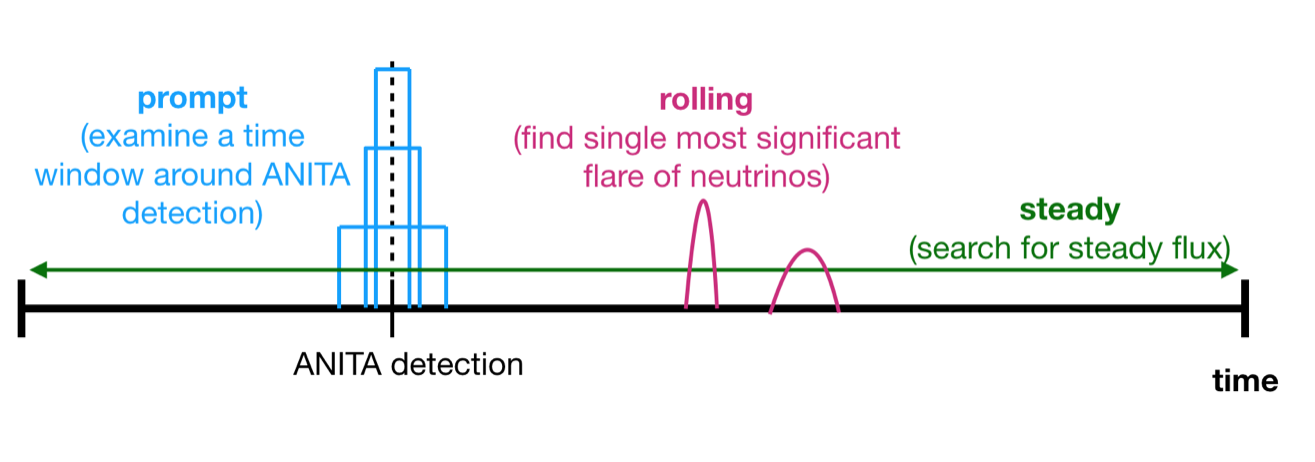
\includegraphics[width=.95\linewidth]{figures/ANITA/ANITA_different_analyses.png}
    \caption[ANITA Analysis types]{Different analysis types for the ANITA point source followup. The prompt analysis searches for IceCube events temporally coincident with the ANITA events, whereas the other analyses relax this constraint while sacrificing time-integrated sensitivity.}
    \label{fig:ANITA:analysis_types}
\end{figure}

\subsection{Prompt Analysis}
\label{ref:subsec:ANITA_prompt}
The prompt analysis focuses on short timescale coincidences. For 99\% containment, the spatial extent of the ANITA PDFs is on the order of around 10 degrees in any given direction. For the event selection used in this analysis \cite{Carver:2019jcd}, the overall event rate is around 4 mHz, meaning the analyses are essentially background free for time windows less than one day (extent is around 1 / 400 of the sky, meaning $4 \mbox{ mHz} \cdot 86400 \mbox{ s} \cdot 0.0025 \approx 1$ event expected in the ANITA PDF per day).

In this regime, TS distributions are characterized by a pileup at TS$=0$, the fraction of which is approximately equal to the proportion of pseudo-experiments in which there is an expectation of zero events in the 99\% containment of the ANITA PDF. So long as the median of this distribution is zero, the sensitivity of this analysis (in $E^2$ scaled time-integrated flux) is constant, and is equal to the flux corresponding to 2.3 signal events, as discussed in Section \ref{sec:poisson_sensitivity}. Distributions for various time-windows are displayed in Figure \ref{fig:ANITA_prompt_bgts}.

\begin{figure}
    \centering
    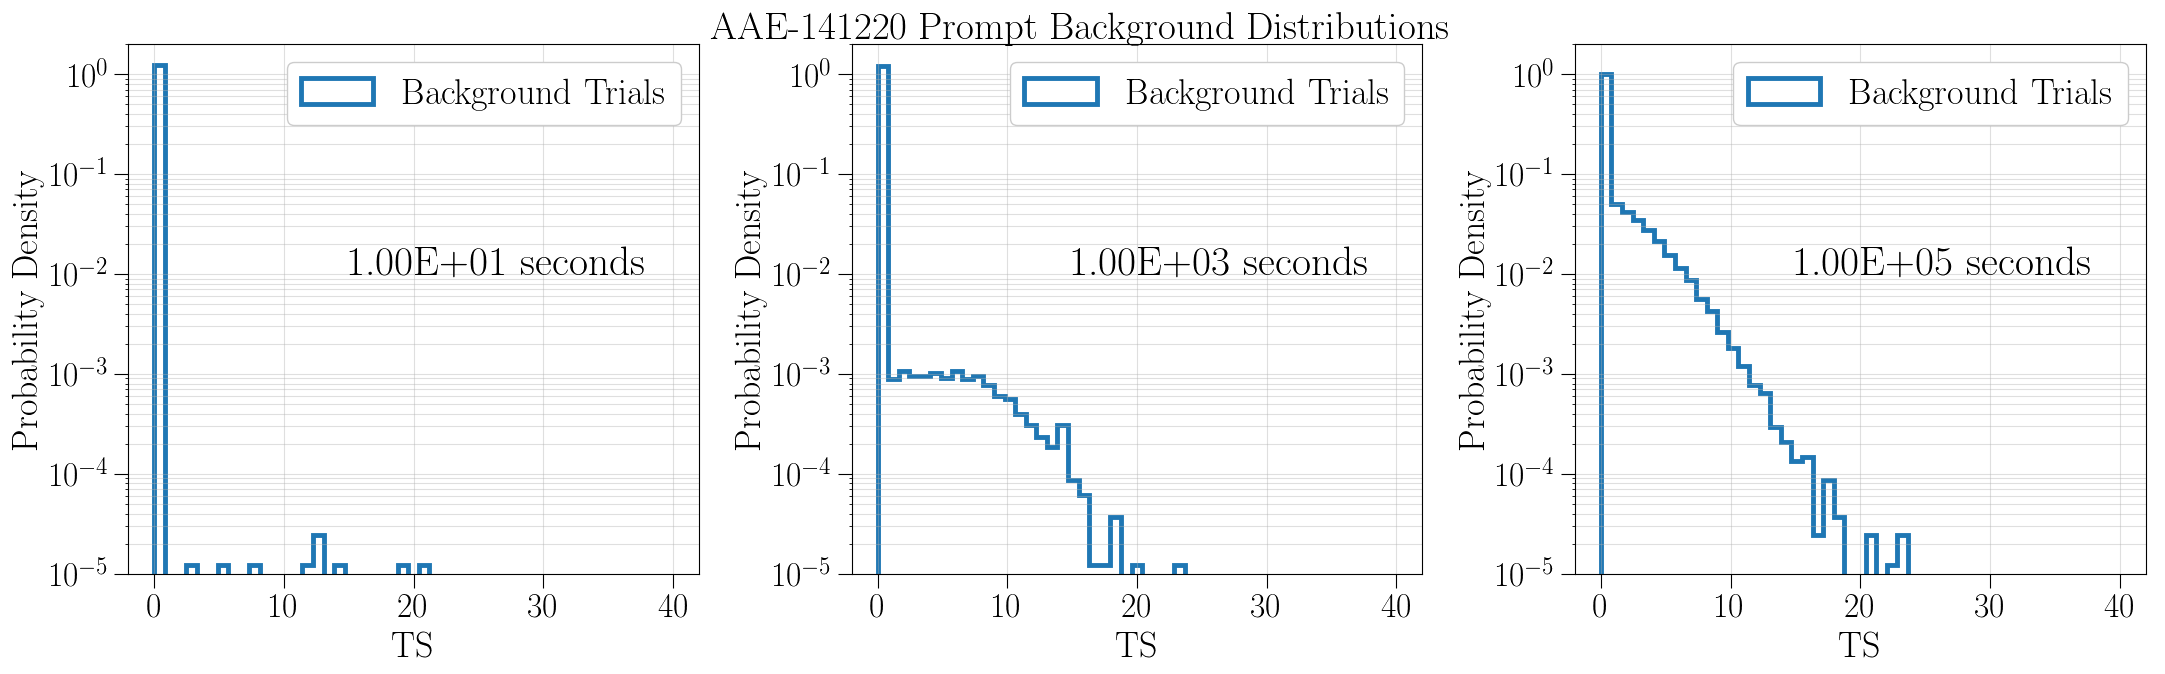
\includegraphics[width=.95\linewidth]{figures/ANITA/Prompt/AAE-141220_background_ts_distributions.png}
    \caption[ANITA Prompt backgroun TS distributions]{Background TS distributions for the short timescale analysis. At the shortest time windows (left), very few coincident background events are expected, leading to most scrambled trials having a TS of 0, whereas at time windows around a day (right), the background becomes non-negligible.}
    \label{fig:ANITA_prompt_bgts}
\end{figure}

Injecting signal on top of this background (as shown in Figure~\ref{fig:ANITA_prompt_sensitivity_fits}) allows one to calculate a sensitivity. These sensitivities are displayed in Figure~\ref{fig:ANITA_prompt_sensitivity}.

\begin{figure}
    \centering
    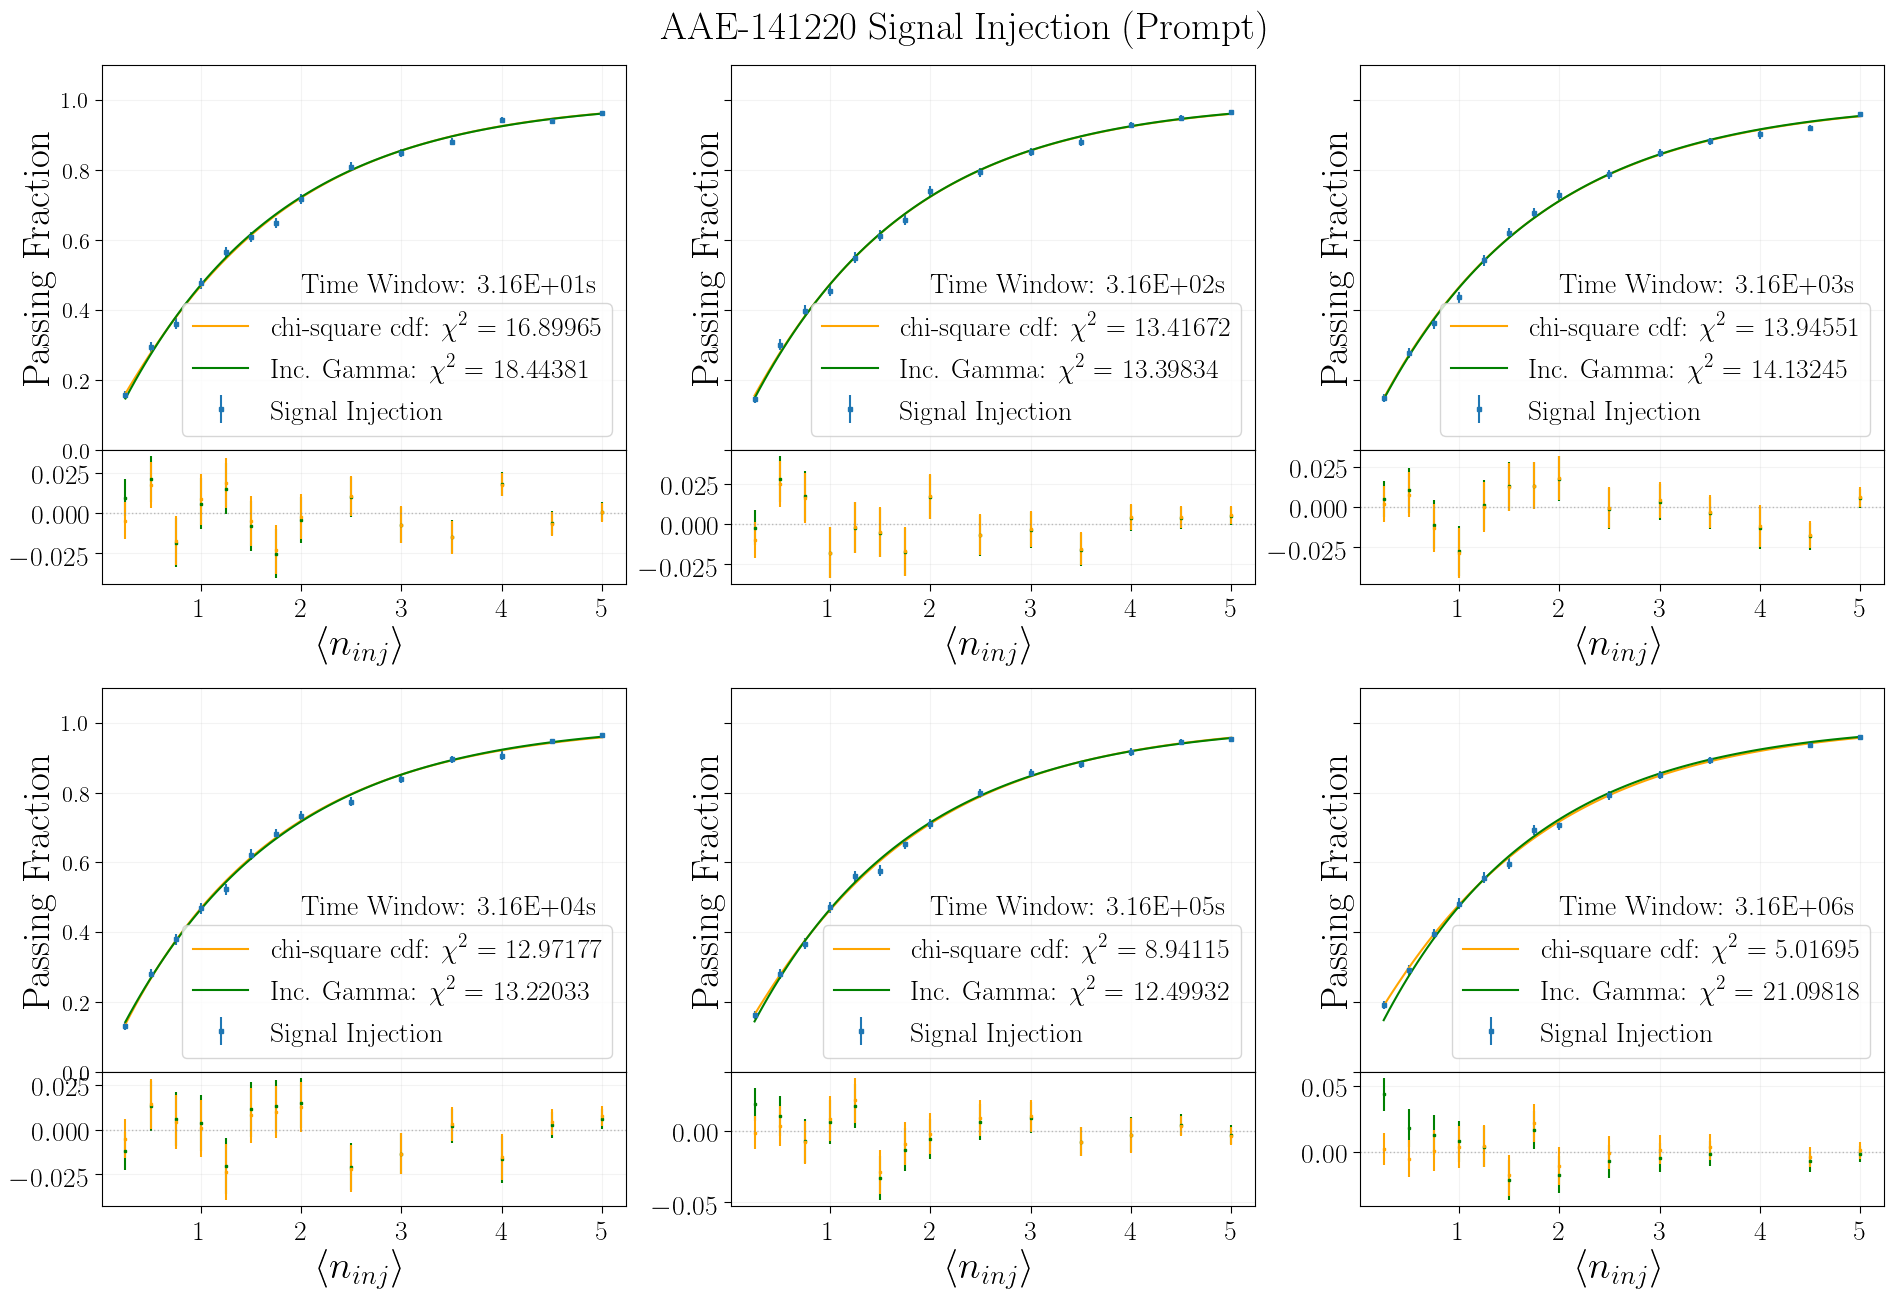
\includegraphics[width=.95\linewidth]{figures/ANITA/Prompt/AAE-141220_prompt_sensitivity_fits.png}
    \caption[ANITA Prompt signal injection]{Signal injection trials for various time windows. The $x$-axis is the average injected number of signal events, and the $y$-axis denotes the fraction of trials which resulted in a TS greater than the median from background only scrambles (such as the ones in Figure~\ref{fig:ANITA_prompt_bgts}. From these, we can extract the sensitivty as the value of $\langle n_{inj} \rangle$ at which the curve crosses 0.9 on the $y$-axis.}
    \label{fig:ANITA_prompt_sensitivity_fits}
\end{figure}

\begin{figure}
    \centering
    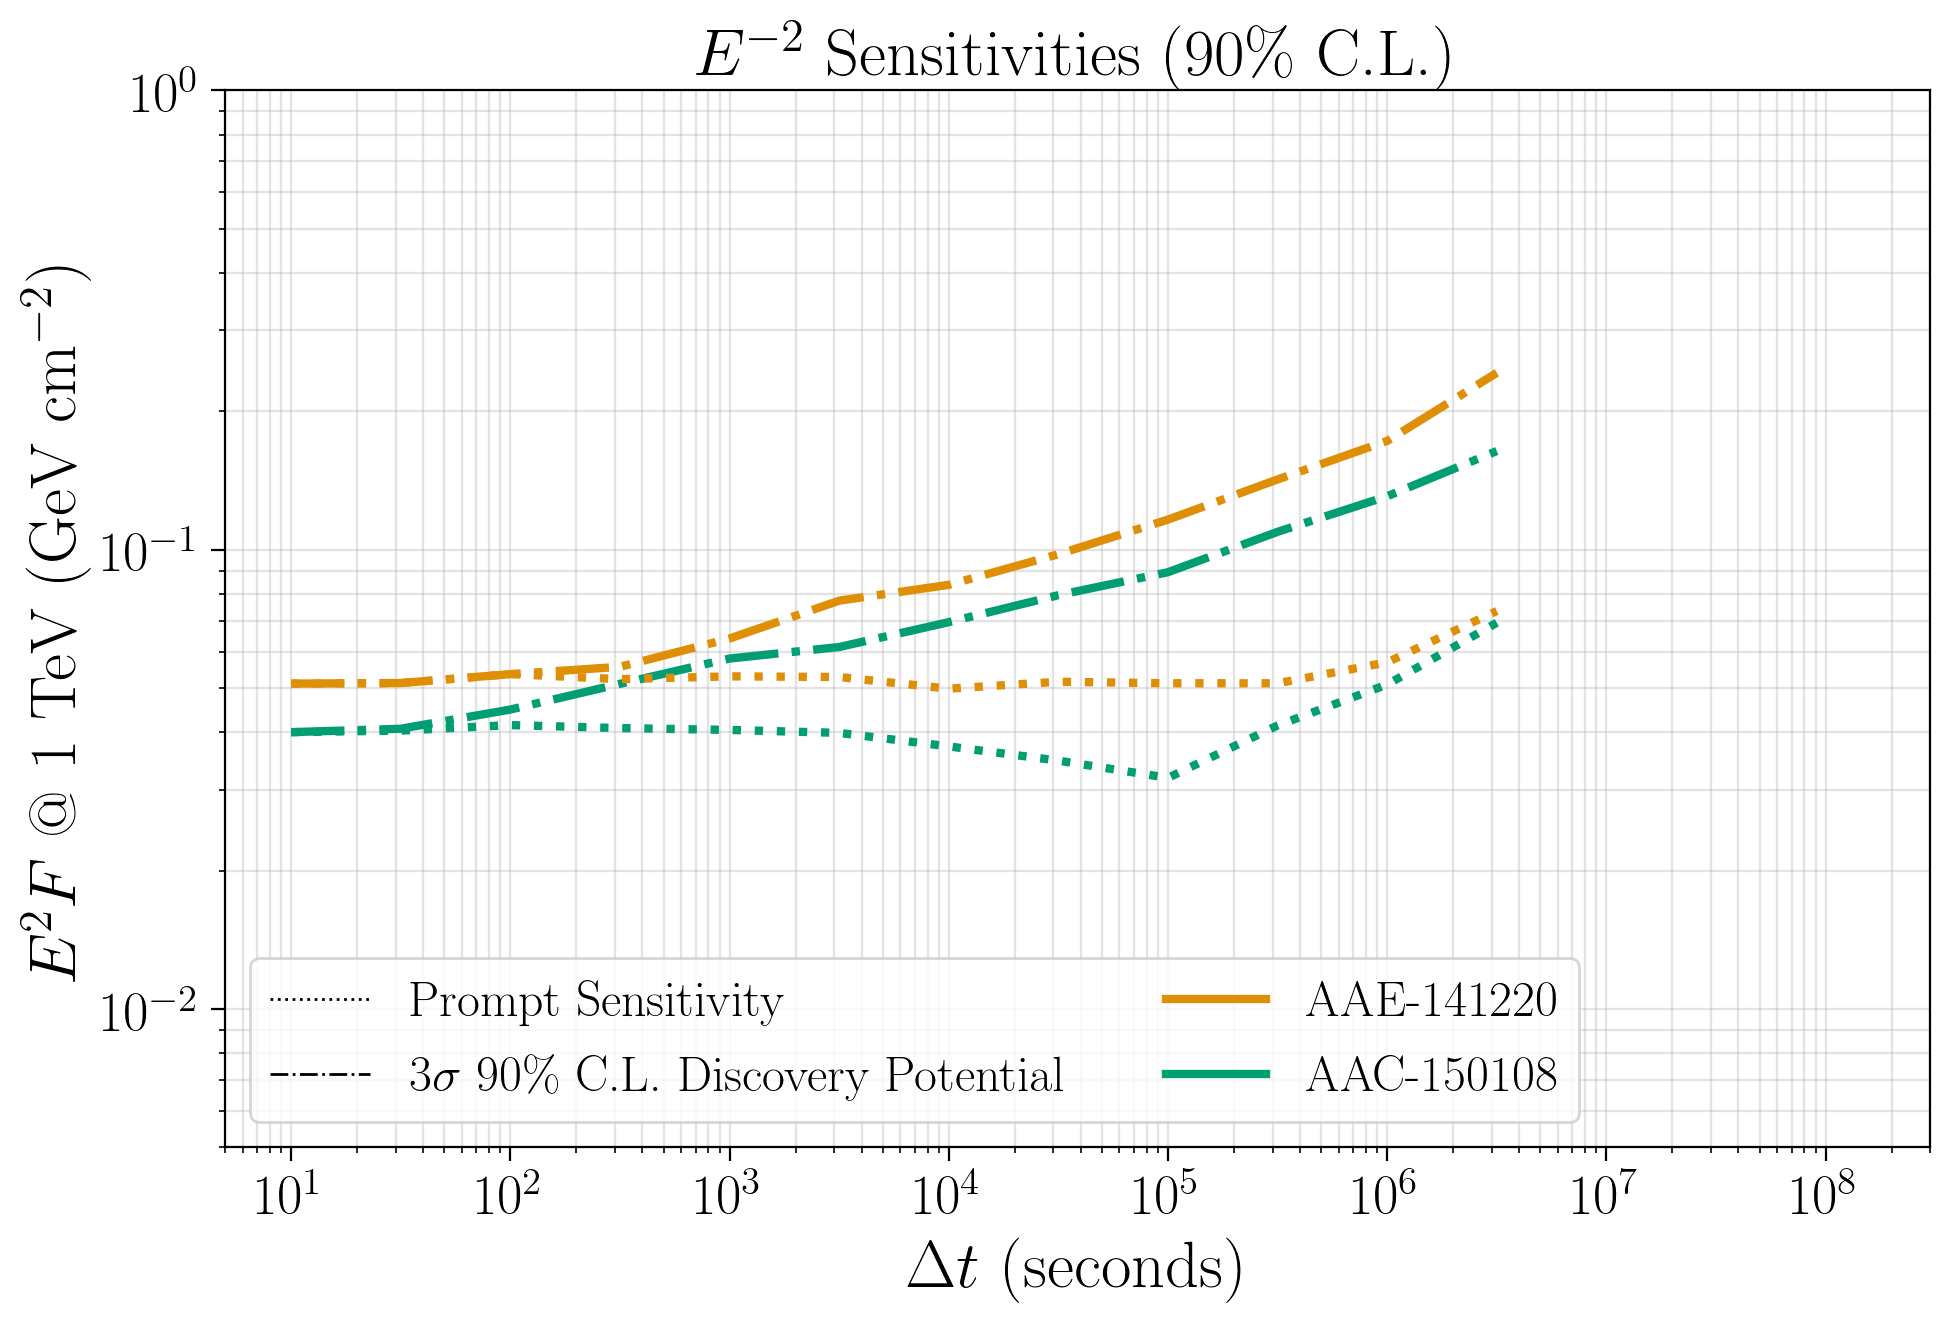
\includegraphics[width=.8\linewidth]{figures/ANITA/Prompt/prompt_sensitivities_no_upper_limits.png}
    \caption[ANITA Prompt sensitivity]{Sensitivity (dotted) and 3$\sigma$ discovery potential (dot dashed) for the two ANITA events for which IceCube had simultaneous observations.}
    \label{fig:ANITA_prompt_sensitivity}
\end{figure}

\subsection{Steady Analysis}
\label{ref:subsec:ANITA_steady}
With the lack of a clear source class and intrinsic timescale of neutrino emission, we also searched for neutrino emission integrated over the entire livetime of the full 86 string detector configuration of IceCube. This section is meant to provide some of the technical plots and details of the analysis. For the full paper, see \cite{Aartsen:2020vir}.

We begin in the same way as the prompt search, by characterizing the background in the analysis. Here, as we are integratinig over multiple years of data and examining a large region of the sky (compared to an ideal point-source), there is a greater probability of fitting non-zero signals when extremizing the likelihoods at every individual pixel. As a result, the background TS distributions are pushed to the right compare to the short timescale, low background case, and this is evident in the distributions in Figure \ref{fig:ANITA_steady_distributions}.

\begin{figure}
    \centering
    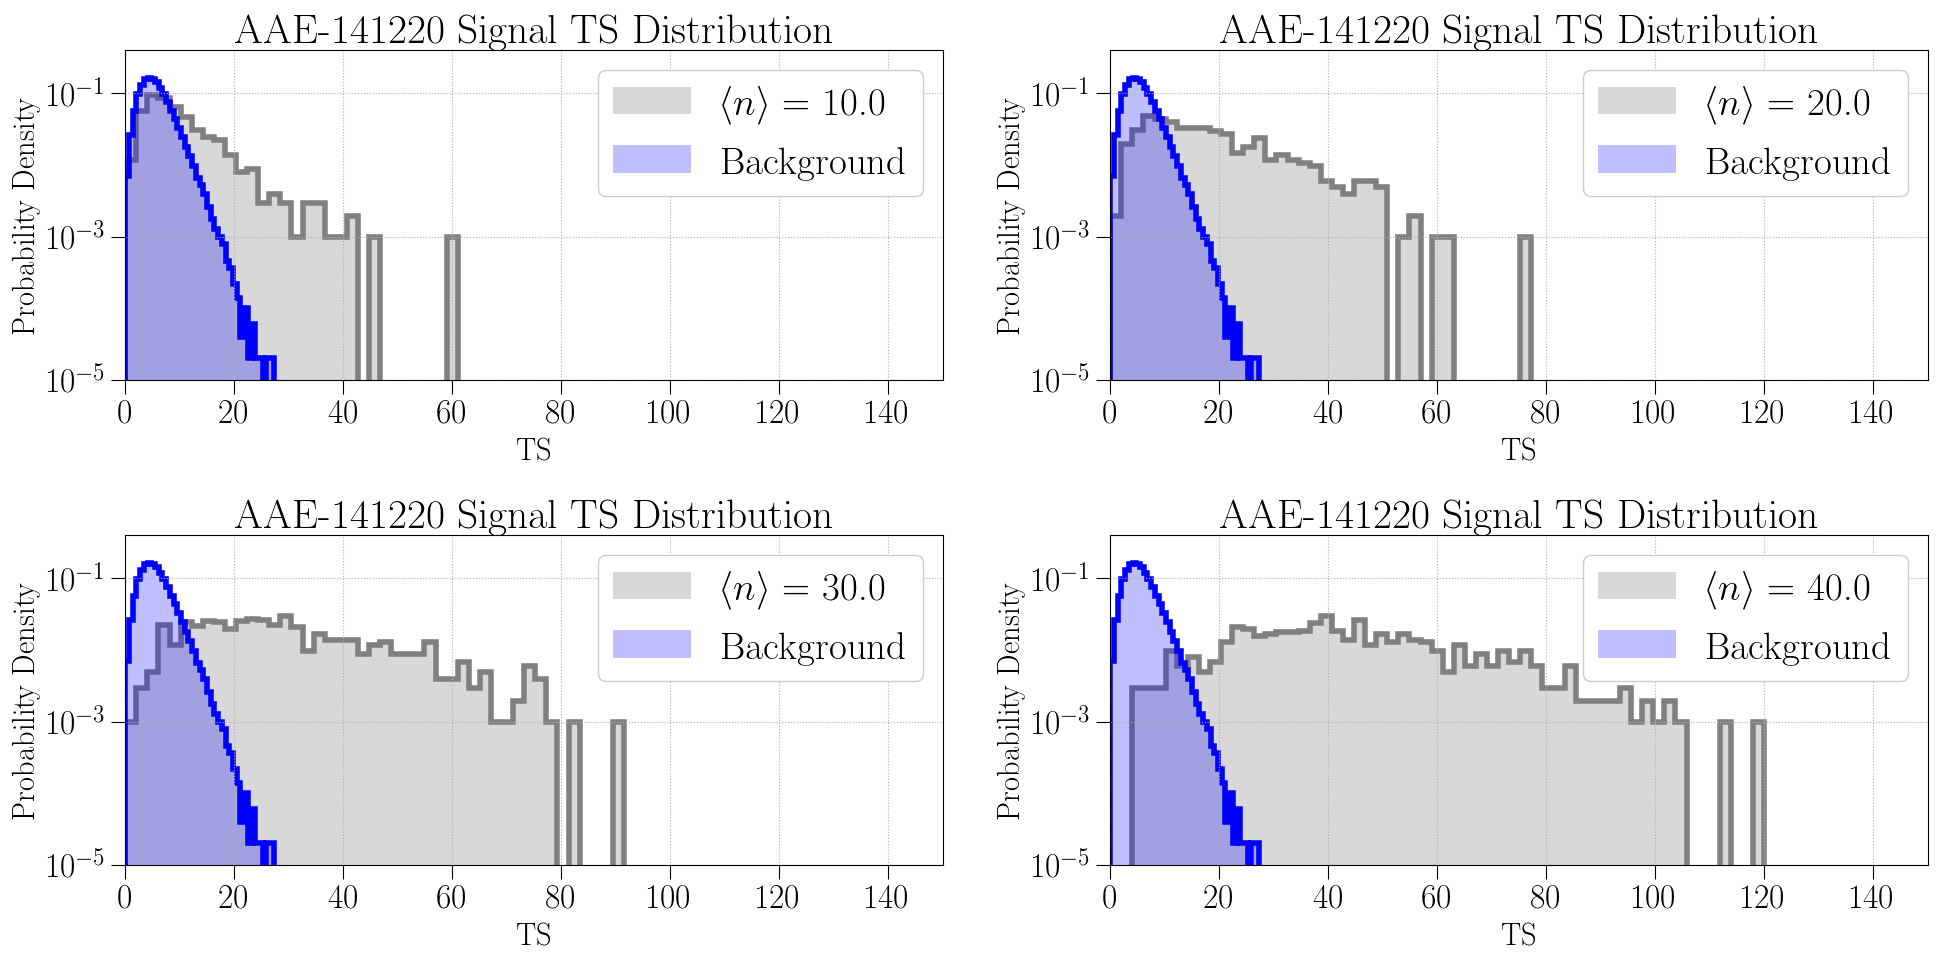
\includegraphics[width=.95\linewidth]{figures/ANITA/Steady/AAE-141220_TS_distributions_with_signal.png}
    \caption[ANITA Steady TS distributions]{Background TS distribution (blue) compared to background + signal distributions (gray). Different panels are with different levels of injected signal. Here, a large signal is required (relative to that of a typical point-source analysis), because of the large source localization uncertainty.}
    \label{fig:ANITA_steady_distributions}
\end{figure}

Sensitivity is then calculated by injecting signal on top of background, following the same procedure as in Section \ref{ref:subsec:ANITA_prompt}. The details of the calculation are displayed in Figure \ref{fig:ANITA_steady_sensitivity}.

\begin{figure}
\centering
\begin{subfigure}
  \centering
  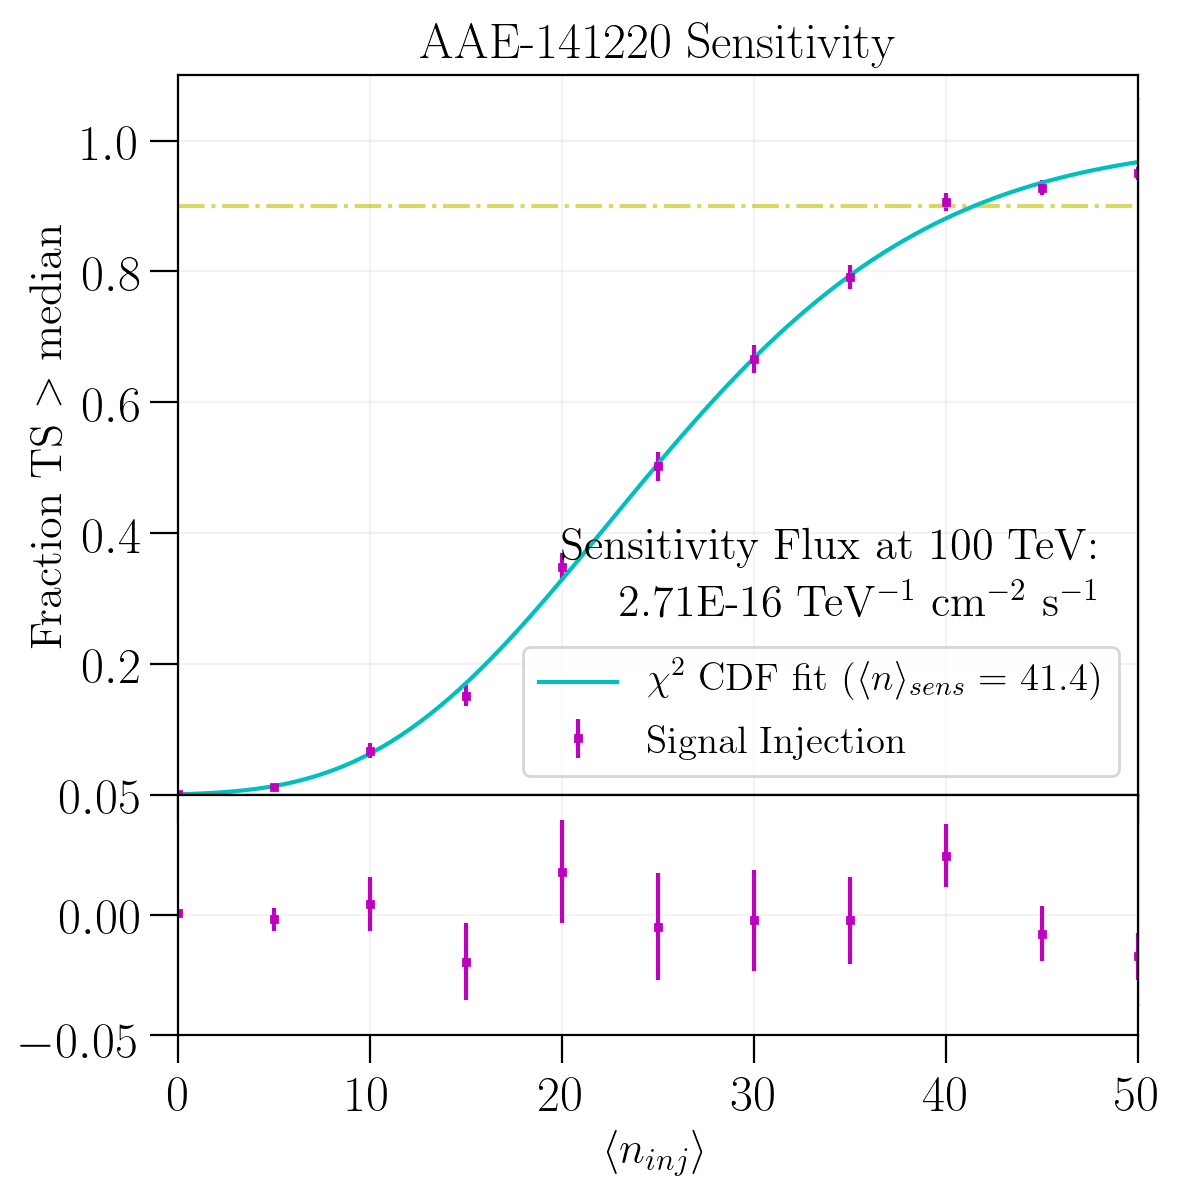
\includegraphics[width=.48\linewidth]{figures/ANITA/Steady/AAE-141220_sensitivity_fits.png}
  %\caption{A subfigure}
  \label{fig:ANITA_steady_sensitivity_fits_aae}
\end{subfigure}%
\begin{subfigure}
  \centering
  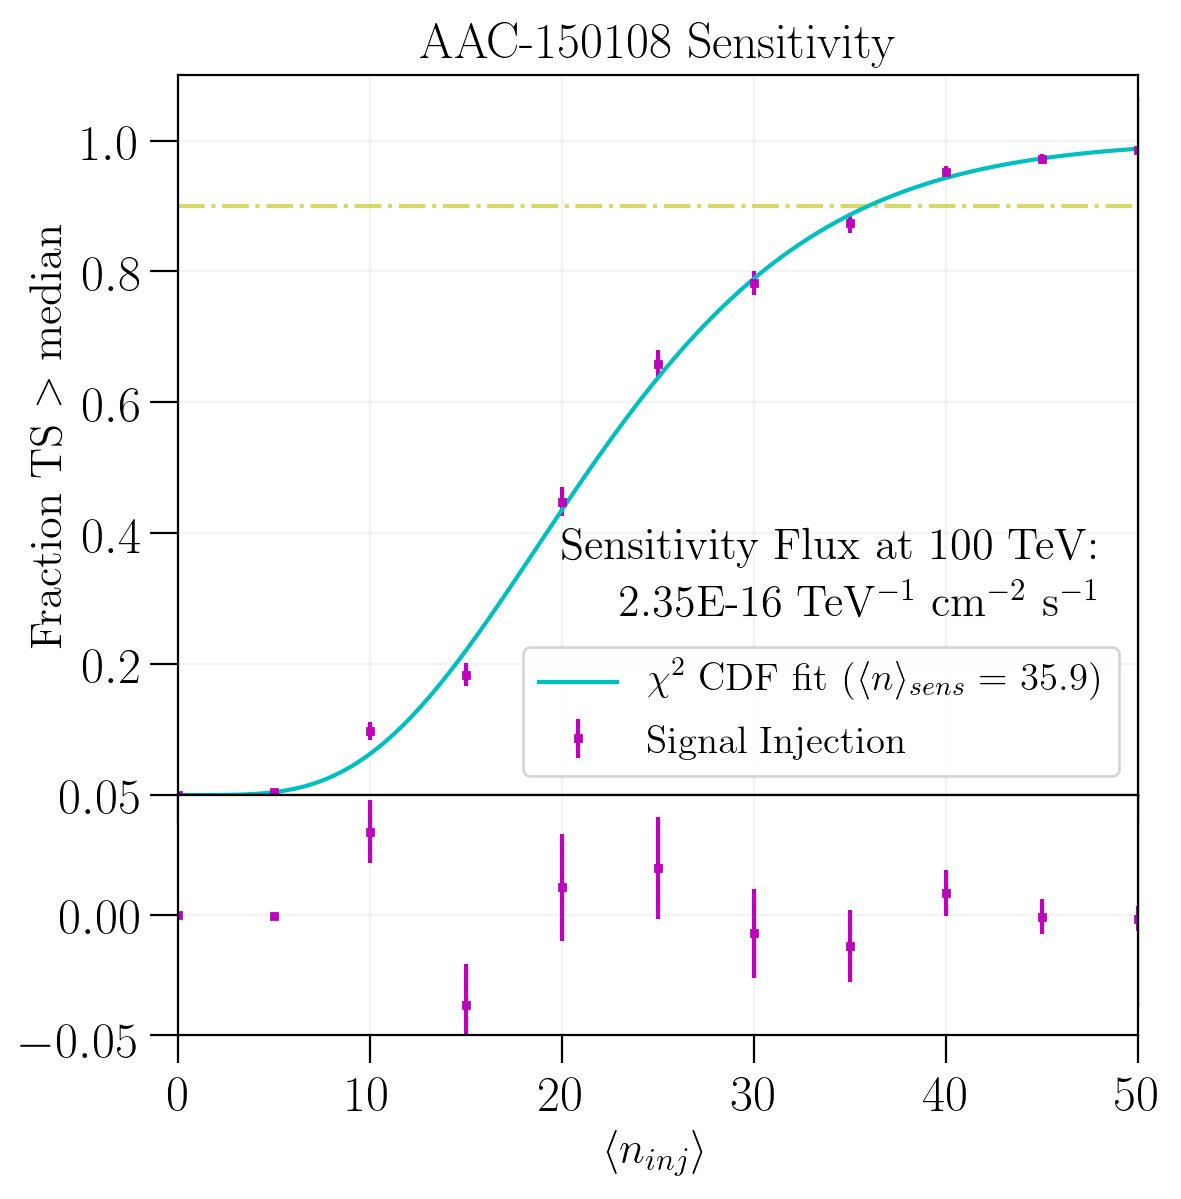
\includegraphics[width=.48\linewidth]{figures/ANITA/Steady/AAC-150108_sensitivity_fits.png}
  %\caption{A subfigure}
  \label{fig:ANITA_steady_sensitivity_fits_aac}
\end{subfigure}
\caption[ANITA Steady sensitivity calculation]{Calculation of sensitivity to time-integrated neutrino emission, performed in the same way as shown in Figure~\ref{fig:ANITA_prompt_sensitivity_fits}}.
\label{fig:ANITA_steady_sensitivity}
\end{figure}

\section{Analysis Results}
\label{sec:ANITA_results}
No significant correlation is found in any of the analyses above the expectation from background. In order to calculate p-values, results are compared against pseudo-experiments from time-scrambled data, namely, the background distributions shown in sections \ref{ref:subsec:ANITA_prompt} and \ref{ref:subsec:ANITA_steady}. The most significant observation results from the steady search for AAE-141220, with a p-value of 0.08 before trials correction.

Figure \ref{fig:ANITA_skymaps} displays the sky maps for the prompt, rolling, and steady analyses from left to right in the top panels for AAE-141220. Bottom panels of Figure \ref{fig:ANITA_skymaps} show the comparison of the observed TS values for each analysis, at the position of the red lines, to their respective TS distributions from pseudo-experiments using time-scrambled data. Similar plots for AAE-061228 and AAC-150108 are displayed in Figure~\ref{fig:ANITA_skymaps_extra}.

\begin{figure*}[t!]
\centering
\vspace{0.0cm}
    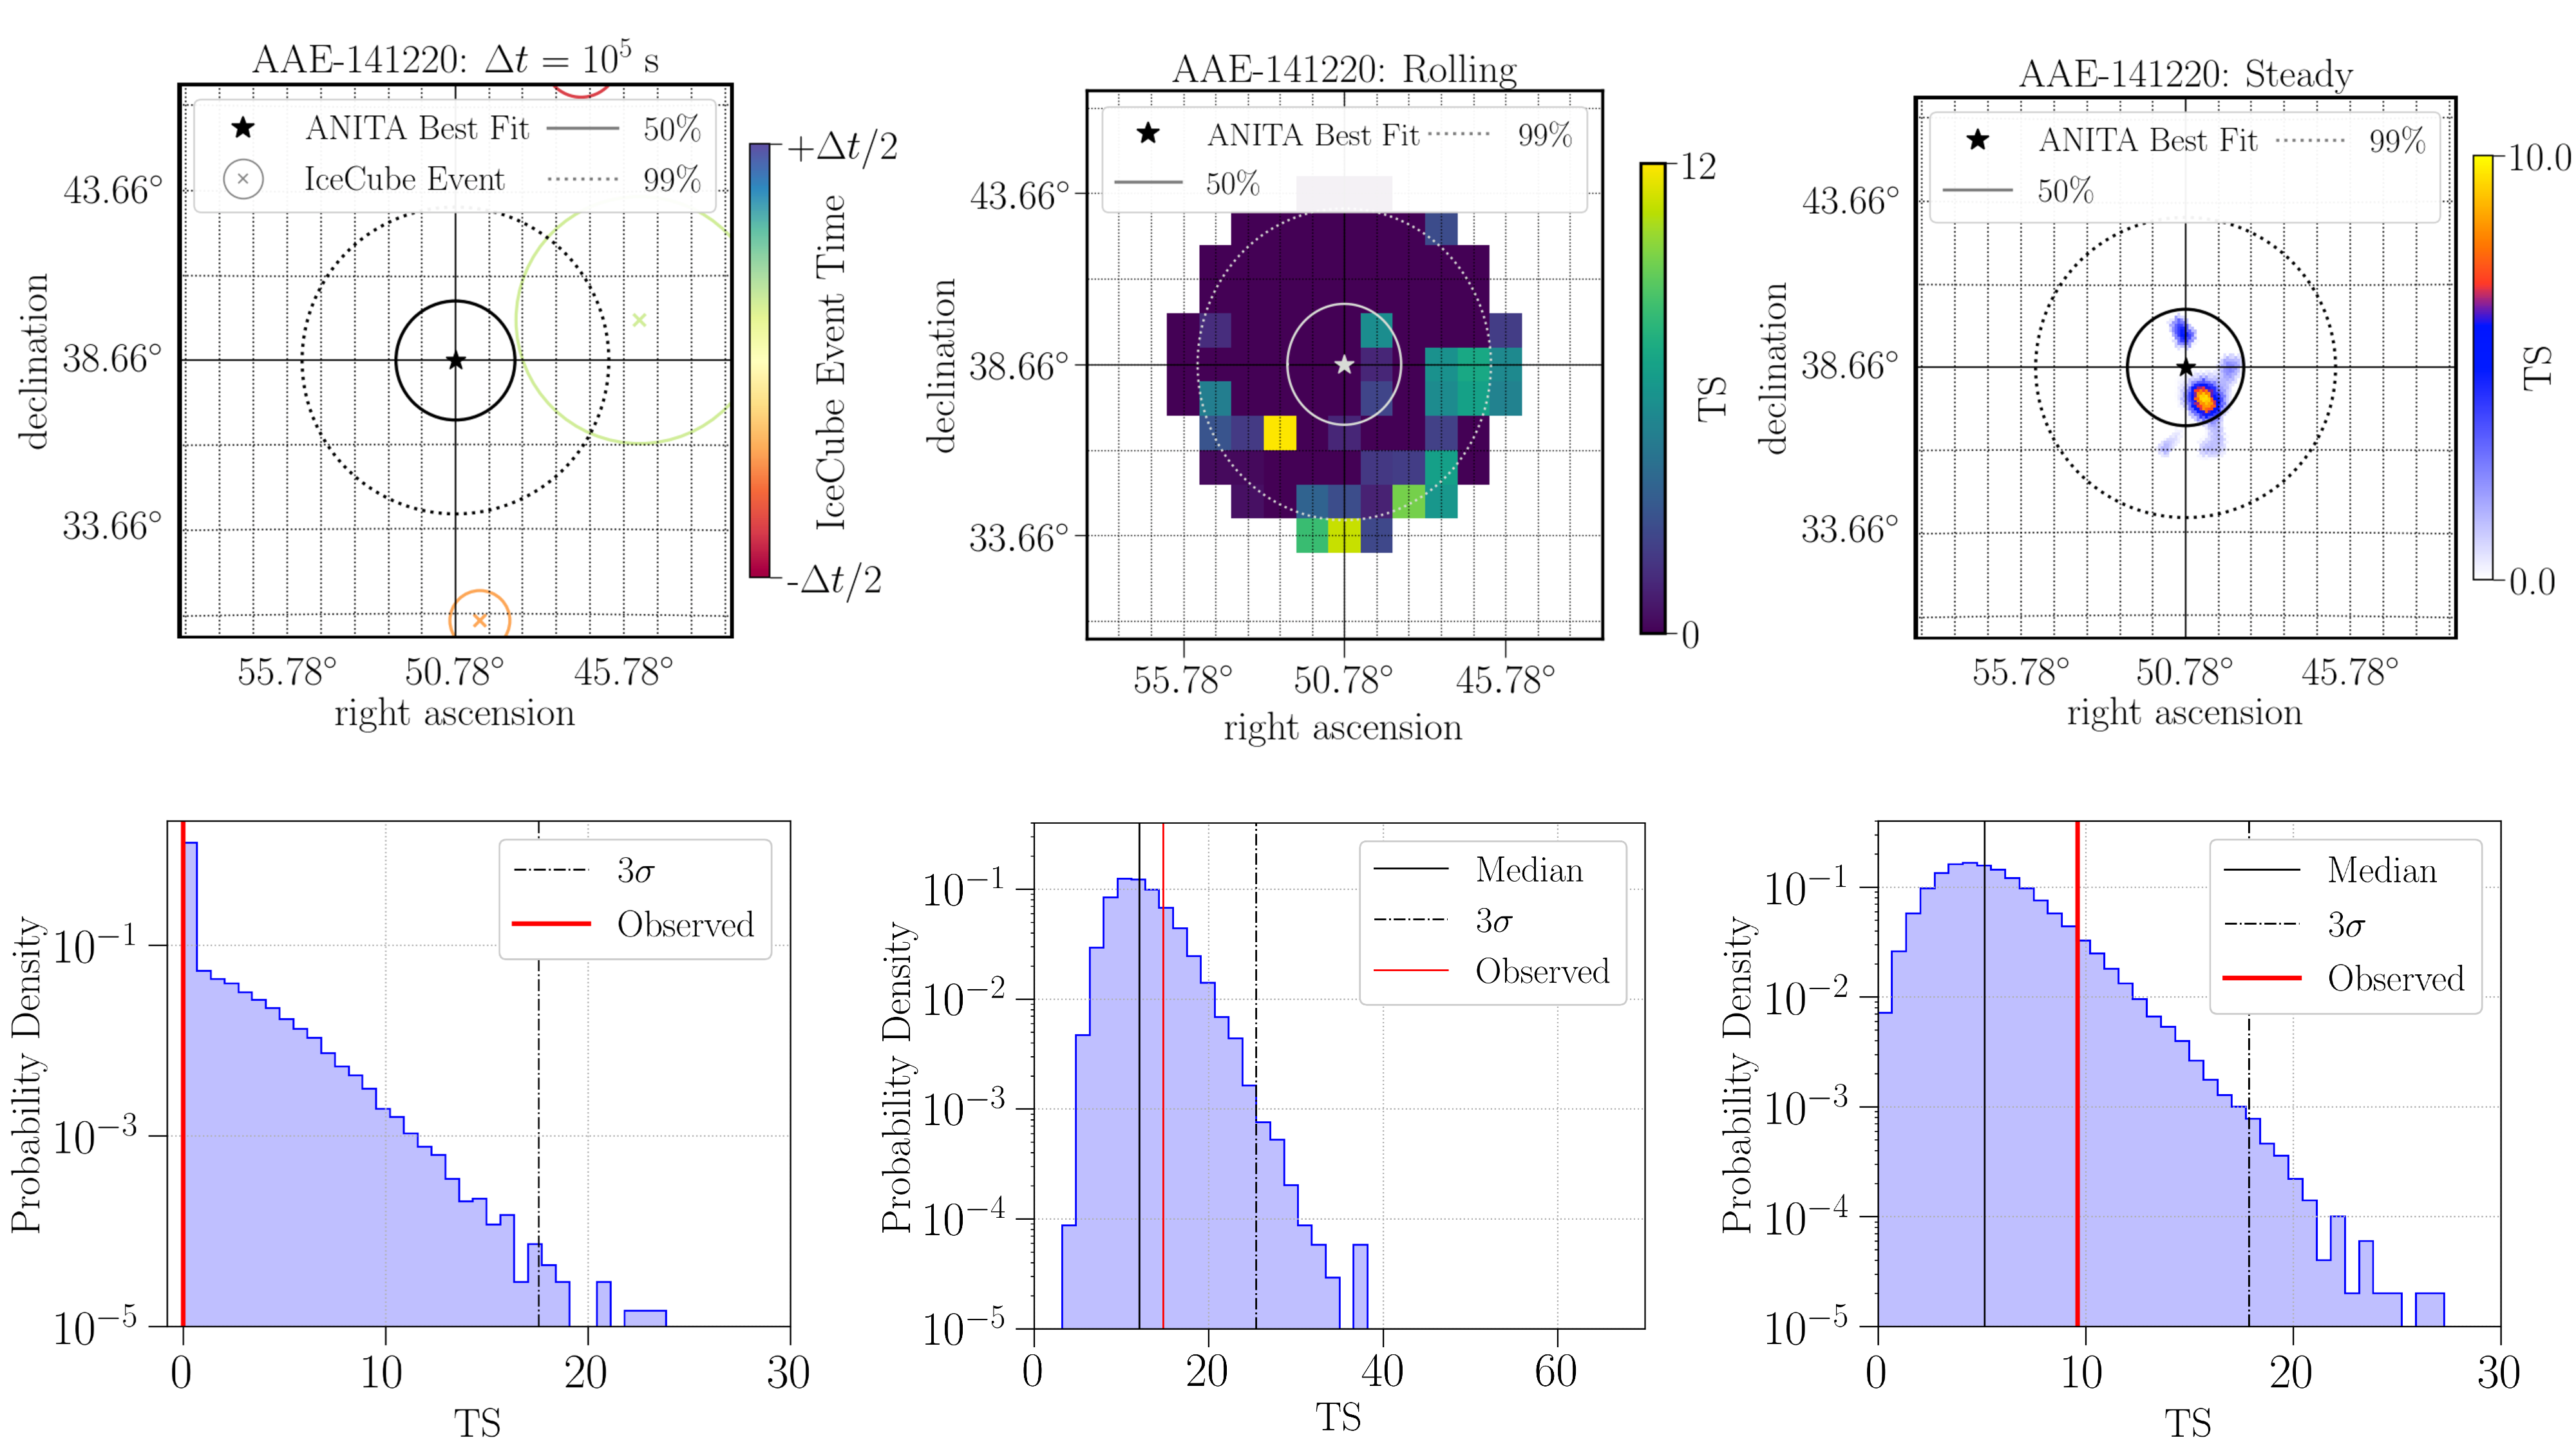
\includegraphics[width=0.99\textwidth=]{figures/ANITA/AAE-141220_collab_paper_plots.pdf}
\caption[AAE-141220 Skymaps]{Sky maps (top) and TS distributions (bottom) for AAE-141220 for the prompt (left), rolling (middle), and steady (right) analyses. Observed TS values (shown in red) are compared to distributions from time-scrambled data realizations to quantify the significance.In all sky maps, solid (dotted) lines represent 50\% (99\%) containment of the reconstructed direction of the events. In the prompt analysis sky map, the best-fit location of each IceCube event is represented with an \texttt{x}, and the size of the circle represents the uncertainty (50\% containment) on the event's reconstruction, with color representing the IceCube event arrival time relative to the ANITA event. Both the sky map and TS distribution for this analysis are for the $10^5$ s time window. In the rolling and steady analysis sky maps, color reflects the TS values. For the details of the rolling analysis, see the full paper attached in Appendix \ref{ANITA-collaboration-paper-appendix}} \label{fig:ANITA_skymaps}
\end{figure*}

\begin{figure*}
    \centering
    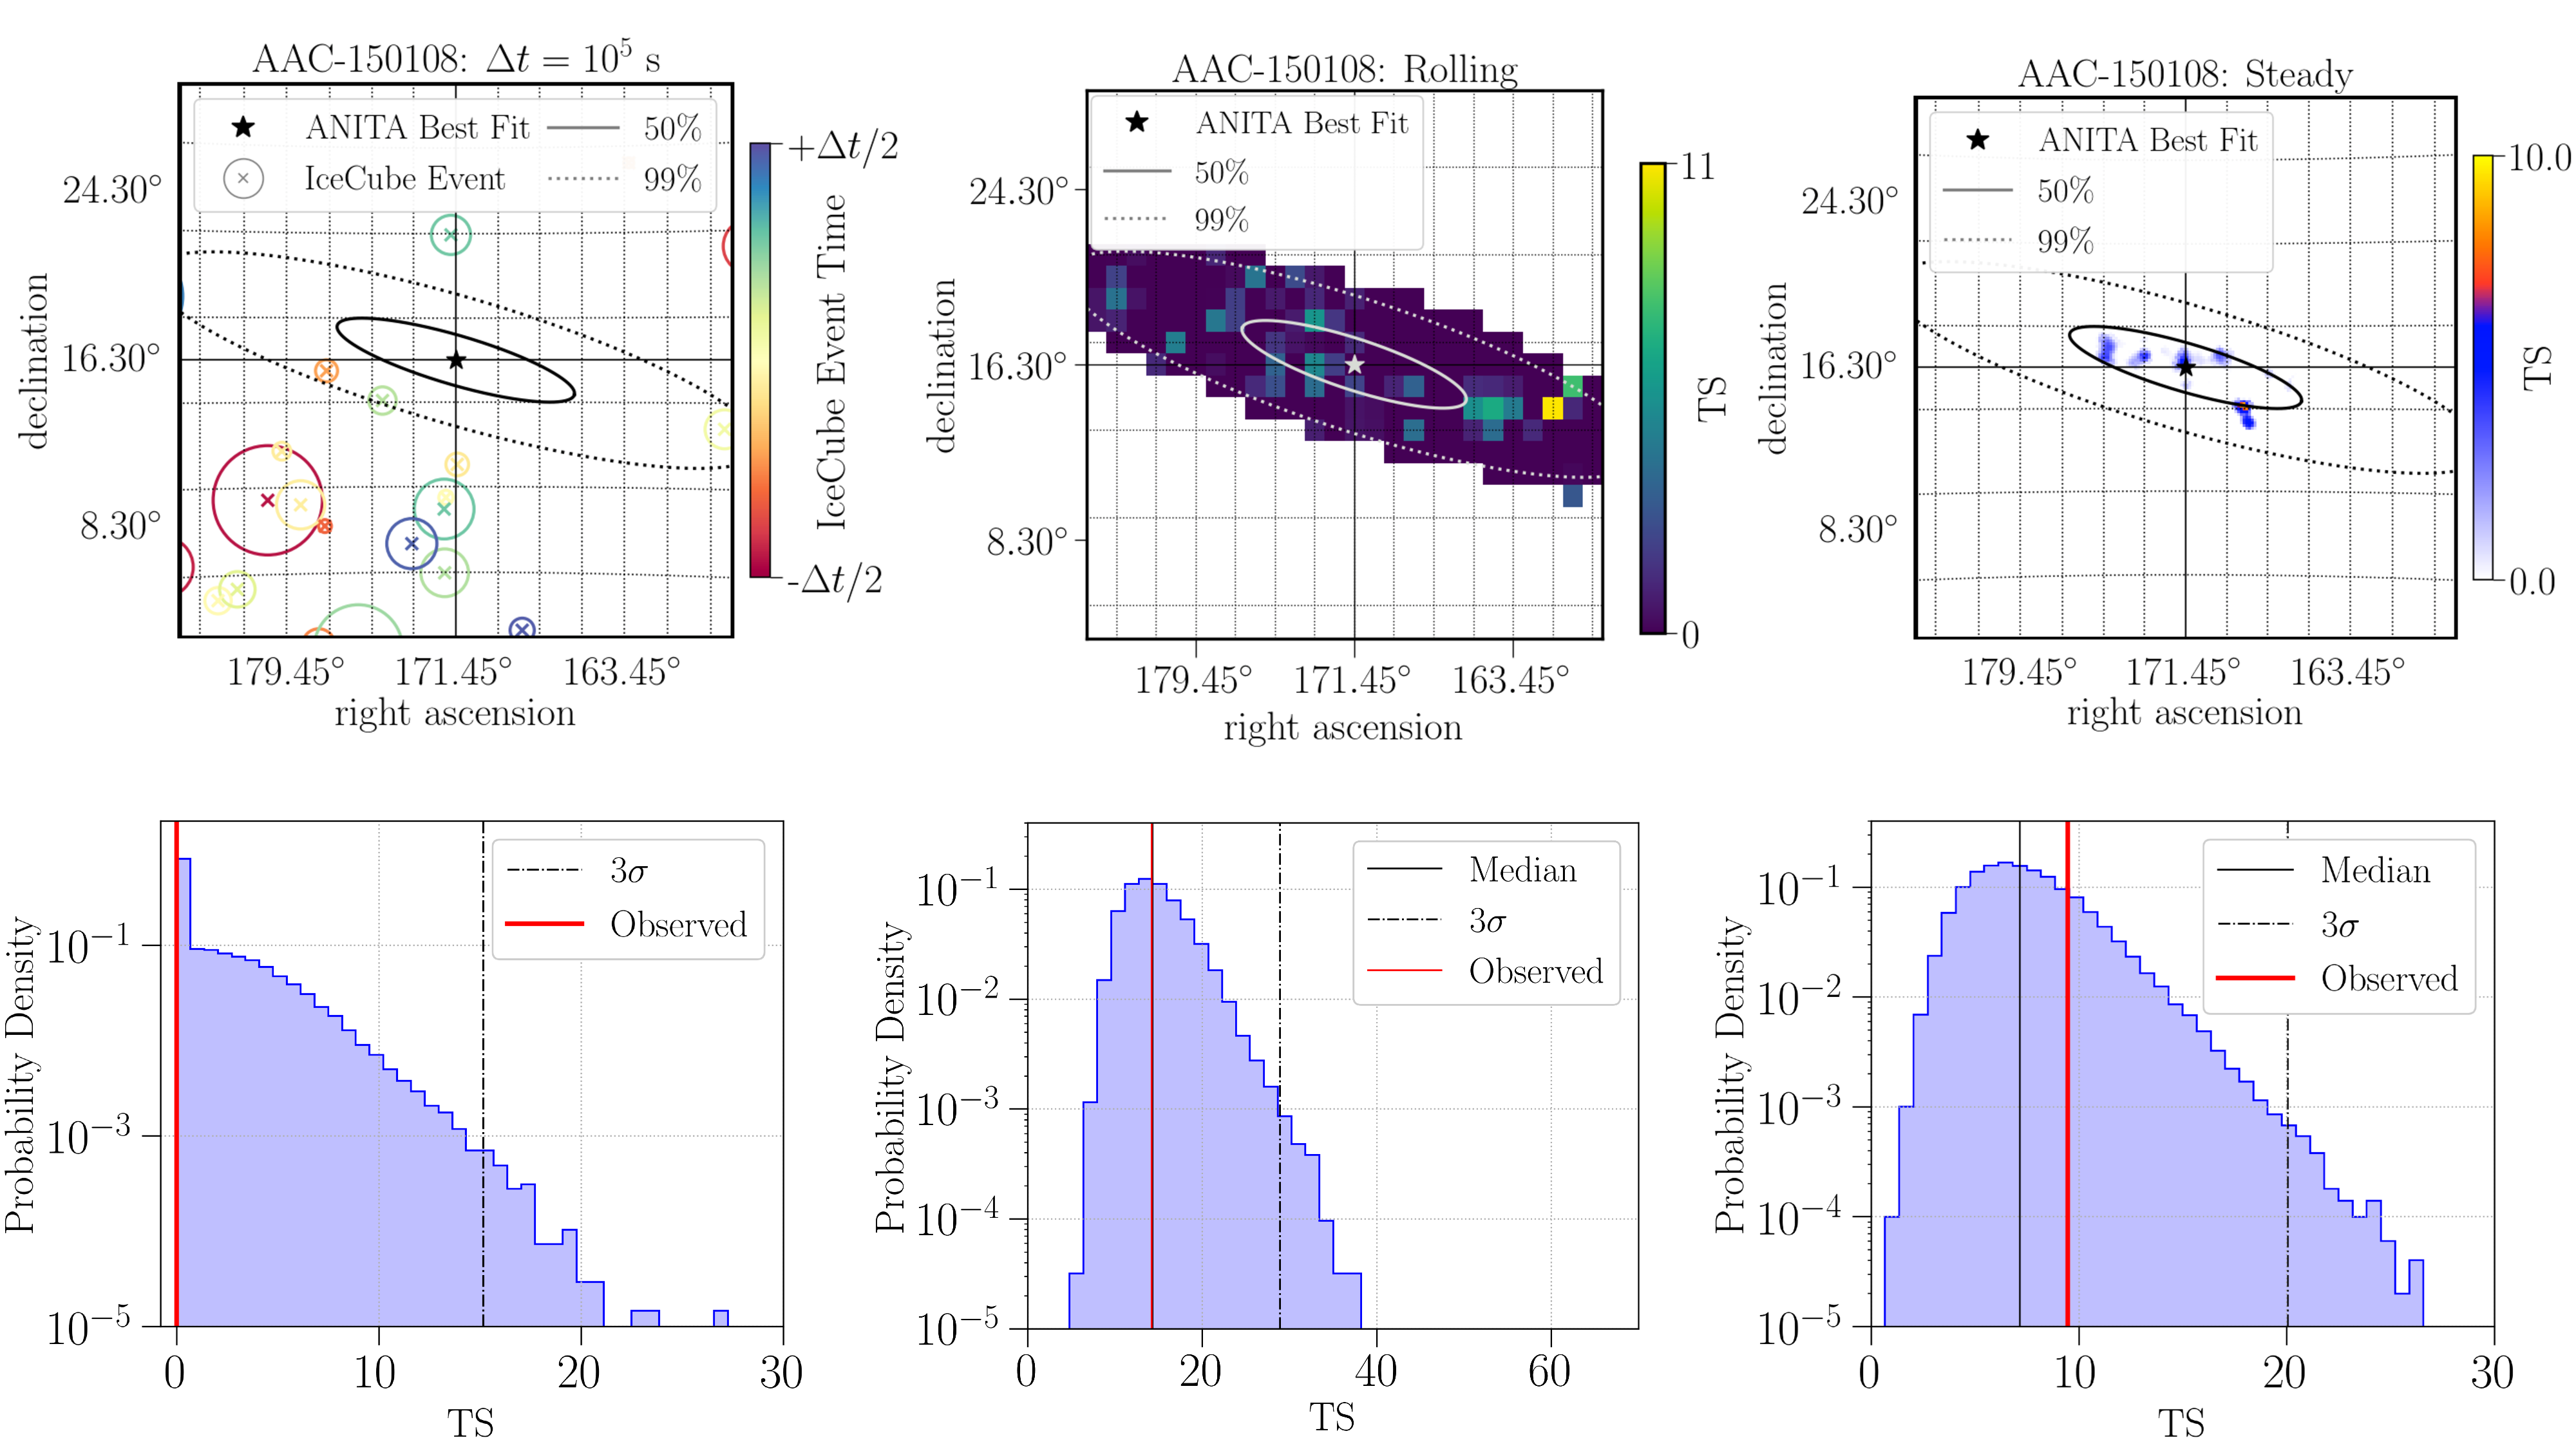
\includegraphics[width=0.99\textwidth]{figures/ANITA/AAC-150108_collab_paper_plots.pdf}
    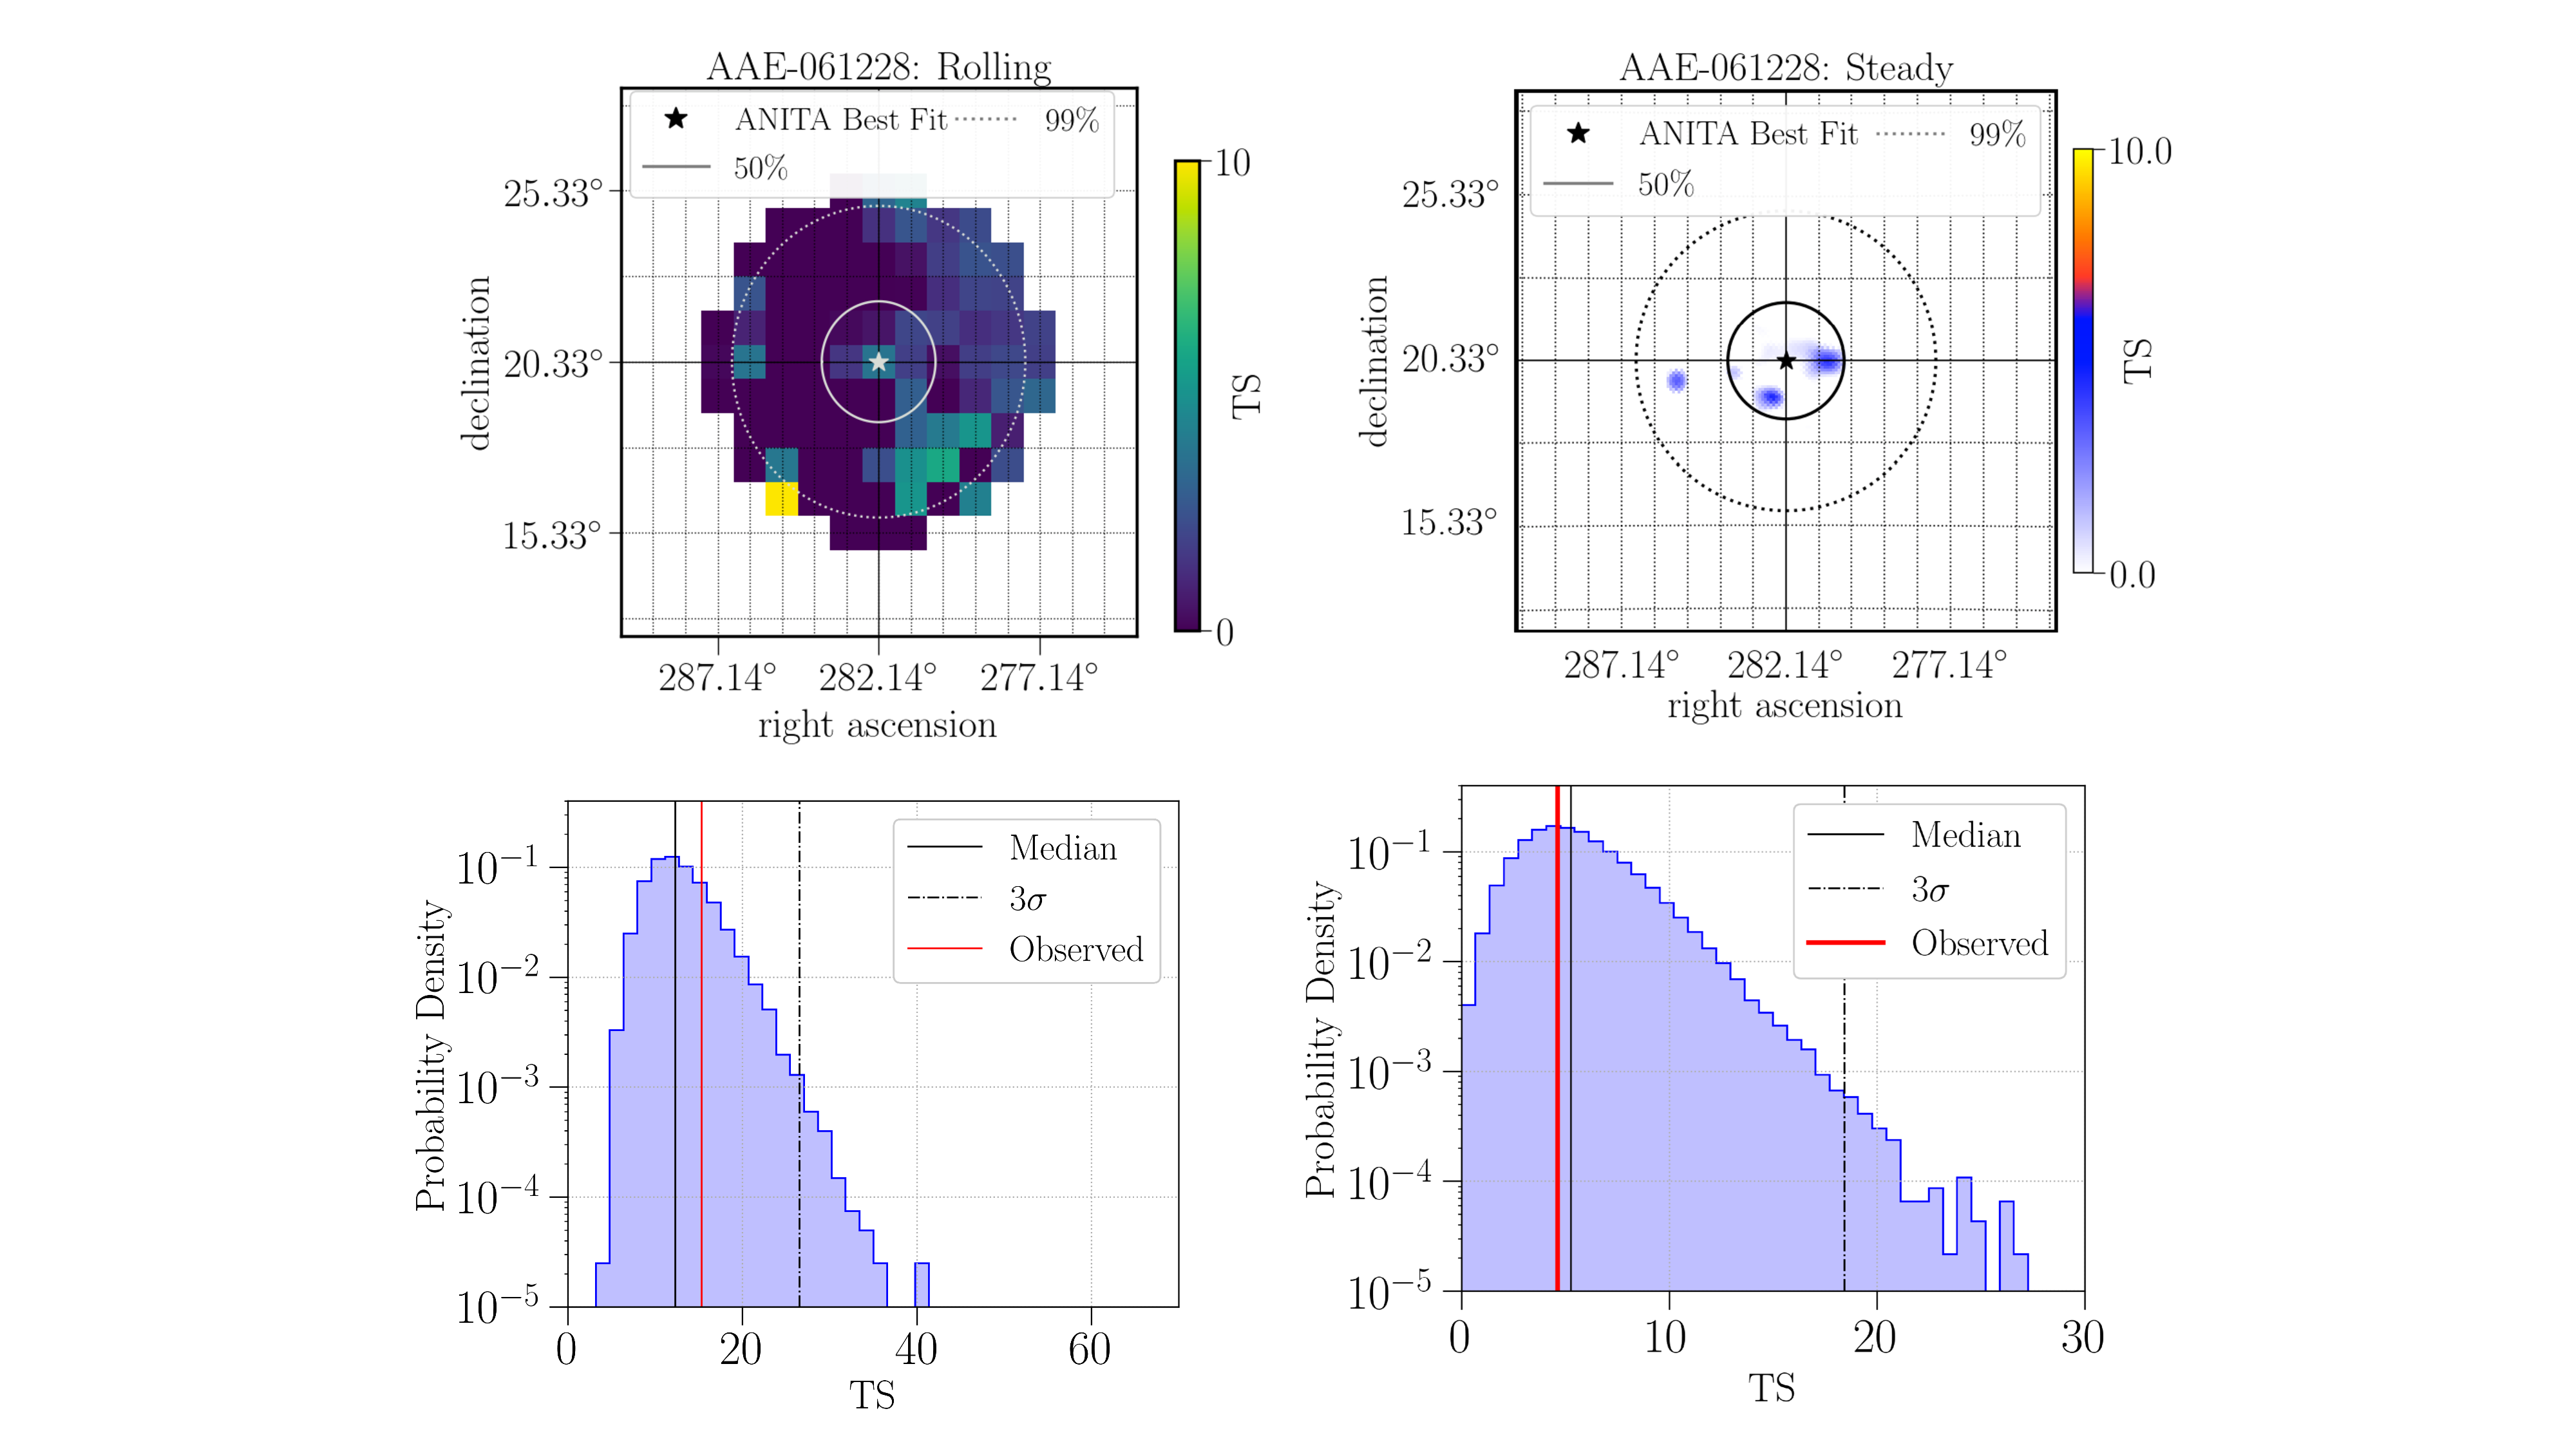
\includegraphics[width=0.99\textwidth]{figures/ANITA/AAE-061228_collab_paper_plots.pdf}
    \caption[AAE-061228 and AAE-150108 Skymaps]{(Top two rows) Skymaps and TS distributions from all three analyses for AAC-150108. For AAE-061228, IceCube was not in a full detector configuration at the time of the event, and thus only the steady and rolling analyses were used to search for neutrino emission. Skymaps and TS distributions for these analyses are displayed in the bottom two rows.} \label{fig:ANITA_skymaps_extra}
\end{figure*}


\begin{figure}
\vspace{0.05in}
\centering
  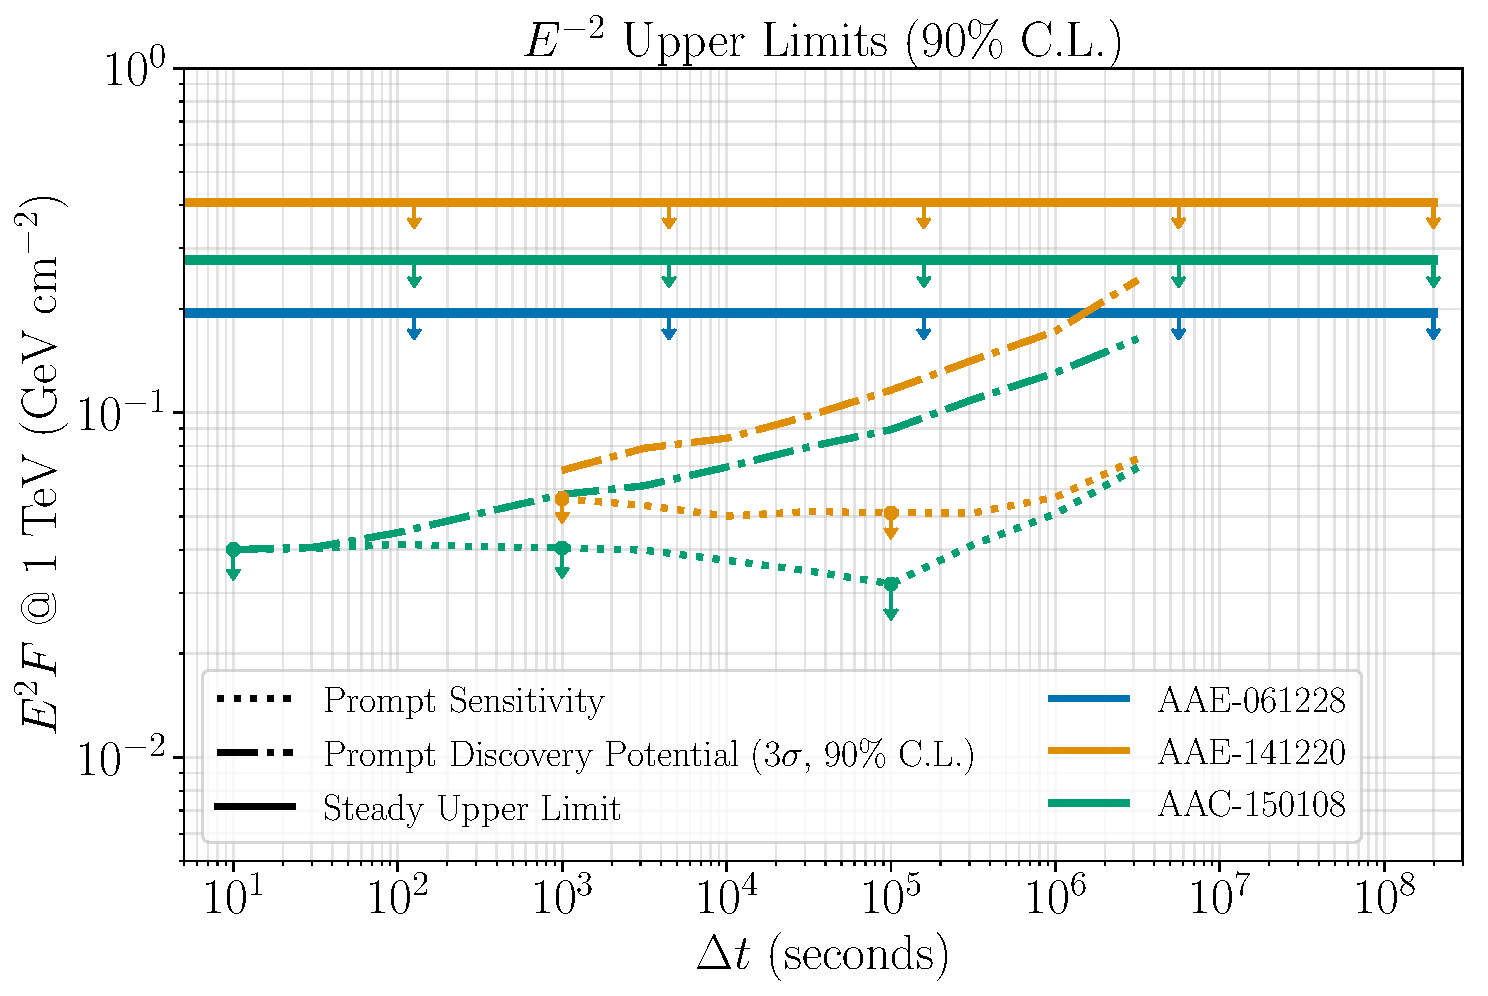
\includegraphics[width=0.7\textwidth]{figures/ANITA/Transient_upper_limits.pdf}
  \label{fig:ANITA_upper_limits}
  \caption[ANITA point source upper limits]{Sensitivity (dotted) and upper limits (arrows) (90\% confidence level) on the time-integrated $\nu_{\mu} + \bar{\nu}_{\mu}$ flux normalization for an $E^{-2}$ source spectrum as a function of $\Delta t$ from the prompt analysis, compared to the upper limits (solid) from the steady analysis. The central 90\% intervals of the expected neutrino energies for these spectra are 1 TeV-1 PeV. \textcolor{black}{For the prompt analysis, we also include the discovery potential, which is the flux that results in a 3$\sigma$ result, pre-trials, in 90\% of pseudo-experiments.}}
\end{figure}

In the absence of a significant signal, upper limits (90\% confidence level) for the time-integrated $\nu_{\mu} + \bar{\nu}_{\mu}$ flux are set for each ANITA event where possible using the prompt and steady analyses (Figure~\ref{fig:ANITA_upper_limits}). To calculate upper limits, locations are sampled according to the per-event PDFs reported by ANITA, injecting the same level of flux at each sampled location, and running each iteration through the full analysis procedure, which maximizes the joint likelihood at all locations in the sky. This allows us to place upper limits on point sources whose locations are distributed according to the per-event PDF reported by ANITA. We set these limits for an assumed spectrum given by
\begin{equation}
    \Phi (E, t) = \frac{\diff N_{\nu_{\mu} + \bar{\nu}_{\mu}}}{\diff E \diff A \diff t} =  \Phi_0 \Big(\frac{E}{E_0}\Big)^{-2} \; , 
\end{equation}
where $\Phi_0$ is a normalization constant on a point-source flux, which carries units of $\rm{GeV}^{-1}\rm{cm}^{-2}\rm{s}^{-1}$. We constrain the time-integrated muon neutrino flux, $E^2F$, where 
\begin{equation}
    E^2 F = E^2 \int \Phi(E, t) \diff t \; .
\end{equation} 
All of the limits we calculate are provided in Table~\ref{tab:results}. In the case that an upper limit fluctuates below the sensitivity, we conservatively set the upper limit to the sensitivity value. Prompt limits are placed at the specified time windows for emission centered on the ANITA event times, whereas limits from the steady analysis are for emission over the live time of our data sample. This hard spectrum was chosen conservatively because with the observation of EeV events by ANITA, if the underlying spectrum is softer, then the expected number of observable neutrinos for IceCube would increase. As the time-integrated flux sensitivity for the triggered analysis begins to worsen past $10^5$ s, upper limits for $\Delta t > 10^5$ s are only set using the time-integrated approach. 

\begin{table*}%[htb!]
    \caption[ANITA analysis results]{Analysis results and upper limits.  Upper limits (90\% C.L) are on the time-integrated $\nu_{\mu} + \bar{\nu}_{\mu}$ power law flux ($E^{-2}$ ) from a point source following the spatial probability distribution provided by ANITA. Limits are set assuming constant emission over a fixed time window. Time windows for the steady and analysis are listed as the IceCube seasons analyzed, where IC86-I contains 2.88$\times 10^7$ s of data and IC86-II--IC86-VII contain 1.90$\times 10^8$ s. All $p$-values are not trial-corrected for the number of searches considered.}
    \centering
    \begin{tabular}{l | c| c| c | c} \hline
     Event & Analysis & Time Window  & $p$-value & Upper limit (GeV $\cdot$ cm$^{-2}$)  \\ \hline \hline
     AAE-061228 & Steady & IC86-I - IC86-VII & 0.606 &  0.195 \\ \hline
     \multirow{3}{*}{AAE-141220} & & 10 s & - & - \\ 
	 & Prompt & $10^3$ s & 1.0 & 0.053 \\ 
	 & & $10^5$ s & 1.0 & 0.051 \\ \cline{2-5}
	 & Steady & IC86-I - IC86-VII & 0.081 & 0.401 \\ \hline
	 \multirow{3}{*}{AAC-150108} & & 10 s & 1.0 & 0.040 \\ 
	 & Prompt & $10^3$ s & 1.0 & 0.041 \\ 
	 & & $10^5$ s & 1.0 & 0.032 \\ \cline{2-5}
	 & Steady & IC86-I - IC86-VII & 0.210 & 0.278 \\  \hline
    \end{tabular}
    \label{tab:results}
    \vspace{0.2in}
\end{table*}

\section{A Joint Interpretation of ANITA and IceCube}
\label{sec:ANITA:joint_interpretation}
This non-observation poses a problem when trying to interpret the ANITA events as astrophysical neutrinos. For most astrophysical sources, fluxes are presumed to follow a spectrum which is falling as a function of energy, and thus a non-observation of neutrinos with TeV - PeV energies is at odds with an observation of neutrinos with $\mathcal{O}$(EeV) energies, especially when the effective area and livetime of IceCube are both greater than that of ANITA for these locations in the Northern sky.

However, the tension is even stronger than that, and even more model independent, because for sources in the Northern sky, \textit{any initial $\nu_{\tau}$ flux with energies greater than 10 PeV will be accompanied by a TeV - PeV $\nu_{\mu}$ flux}. Thus, our non-observation constrains even the most finely tuned Standard Model fluxes which could result in an EeV $\nu_{\tau}$ reaching the ANITA detector. 

This is a result of \nutau regeneration. When a high energy \nutau interacts with a nucleon via a CC interaction, a $\tau$ lepton is produced which carries a significant fraction of the initial \nutau energy. This $\tau$ then decays, with characteristic decay length of about 50 m$/$PeV. When the $\tau$ decays, another \nutau is produced, in addition to possible other flavors of neutrino (see diagram below).

\begin{center}
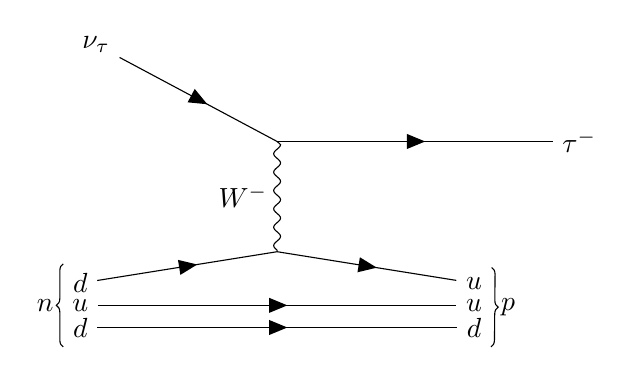
\begin{tikzpicture}
\begin{feynman}
\vertex (d1) {\(d\)}; 
\vertex[right=5cm of d1] (u3) {\(u\)}; 
\vertex[below=0.8em of d1] (u1) {\(u\)}; 
\vertex[right=5cm of u1] (u2) {\(u\)};
\vertex[below=0.8em of u1] (d2) {\(d\)}; 
\vertex[right=5cm of d2] (d3) {\(d\)};
\vertex[above right=0.4cm and 2.5cm of d1] (v1);
\vertex[above=1.4cm of v1] (v2);
\vertex[above left=1cm and 2cm of v2] (nu) {$\nu_{\tau}$};
\vertex[right=3.5cm of v2] (e) {$\tau^-$};
\diagram* { {[edges=fermion]
(d1) -- (v1) -- (u3), (u1) -- (u2),
(d2) -- (d3), (nu) -- (v2) -- (e)},
(v1) -- [boson, edge label=\(W^{-}\)] (v2)
};
\draw [decoration={brace}, decorate] (d2.south west) -- (d1.north west) node [pos=0.5, left] {\(n\)};
\draw [decoration={brace}, decorate] (u3.north east) --  (d3.south east) node [pos=0.5, right] {\(p\)};
\end{feynman} 
\end{tikzpicture}
\begin{tikzpicture}
\begin{feynman}
\vertex (a) {\(\tau^{-}\)};
\vertex [right=of a] (b);
\vertex [above right=of b] (f1) {\(\nu_{\tau}\)};
\vertex [below right=of b] (c);
\vertex [above right=of c] (f2) {\(\overline \nu_{e},\overline \nu_{\mu},\overline u\)};
\vertex [below right=of c] (f3) {\(e^{-},\mu^{-},d\)};
\diagram* {
(a) -- [fermion] (b) -- [fermion] (f1),
(b) -- [boson, edge label'=\(W^{-}\)] (c),
(c) -- [anti fermion] (f2),
(c) -- [fermion] (f3),
};
\end{feynman}
\end{tikzpicture}
\end{center}

This secondary \nutau often carries a significant fraction of energy of the initial \nutau, and this secondary \nutau flux will develop and pileup at energies around 100 TeV. The secondary flux does not cascade down to energies lower than this value, because at this energy the Earth becomes transparent, and the \nutau flux is no longer likely to interact before reaching a detector such as IceCube. 

Initial \nutau fluxes can then be constrained by looking for the $\mu$ from $\tau$ decay. For a more detailed description of the properties of secondary fluxes, see the full paper attached in Appendix \ref{APPENDIX WITH FEW AUTHOR PAPER}.

Using this technique to constrain the ANITA events, we found the initial \nutau energy that was most likely to result in a detection at ANITA, and inject the most finely tuned flux (namely a delta function), floating its normalization until the observation of an event at ANITA is expected, where the number of events expected at ANITA is given by

\begin{equation}
    \langle N ^ { \tau }_{\mathrm{ANITA}} \rangle = \iint \Big( \diff E _ { \nu } \diff E^{\prime} _ { \nu } \Phi \left( E _ { \nu }, t \right) \frac { \diff N \left( E^{\prime} _ { \nu } \right) } { \diff E^{\prime} _ { \nu } } \times \xi _ { a c c } \left( E^{\prime} _ { \nu } \right) \Delta T \Big) ,
\end{equation}

where $\xi_{acc}$ represents ANITA's acceptance to $\tau$-lepton air showers, taken from \citep{Romero-Wolf:2018zxt}. We then use the secondary \nutau flux from this injected delta function spectrum, and calculate the number of events we would see from $\tau$ decay to $\mu$ in IceCube, given by

\begin{align}
\langle N _ { \text {IceCube} } ^ { \mu } \rangle & = \int \diff E _ { \mu } \int \diff E _ { \tau } \int \diff E _ { \nu } \Phi \left( E _ { \nu }, t \right) P _ { \tau } ^ { s u r v } \left( E _ { \nu } \right) \frac { \diff N _ { \tau } \left( E _ { \tau } \right) }{ \diff E _ { \tau } }  \\
& \qquad \frac{\Gamma_{\tau\rightarrow\mu}}{\Gamma_{\rm{total}}} \frac { \diff N _ { \mu } } { \diff E _ { \mu } } \left( E _ { \tau } , E _ { \mu } \right) A _ { e f f } ^ { \mu } \left( E _ { \mu } \right) \Delta T \nonumber
\\ & + \int \diff E _ { \mu } \int \diff E _ { \tau } \int \diff E _ { \nu } ^ { \prime } \int \diff E _ { \nu } \Phi \left( E _ { \nu }, t \right) P _ { \nu } \left( E _ { \nu } , E _ { \nu } ^ { \prime } \right) \frac { \diff N _ { \nu } } { \diff E _ { \nu } ^ { \prime } } \left( E _ { \nu } ^ { \prime } \right) \nonumber \\ 
& \qquad N^{p} \left( E^{\prime}_{\nu} \right) \frac { \diff N _ { \tau } } { \diff E _ { \tau } } \left( E ^{\prime} _ { \nu} ; E _ { \tau} \right)  \frac{\Gamma_{\tau\rightarrow\mu}}{\Gamma_{\rm{total}}} \frac { \diff N _ { \mu } } { \diff E _ { \mu } } \left( E _ { \tau} ; E _ { \mu} \right) A _ { e f f } ^ { \mu } \left( E _ { \mu } \right) \Delta T \; , \nonumber
\end{align}

where the first contribution is from emerging tau-leptons that would decay to muons and then pass an IceCube event selection. The second contribution is from the remaining $\nu_{\tau}$ flux, the majority of which has cascaded down in energy. $N^{p} (E_{\nu})$ is the number of targets effectively seen by an incident neutrino with energy $E_{\nu}$. $P _ { \tau } ^ { s u r v } \left( E _ { \nu } \right)$ and $P _ { \nu }(E _ { \nu })$ represent the survival probability of a $\tau$-lepton and $\nu_{\tau}$, given an incident neutrino energy, respectively, and $\Gamma_{\tau\rightarrow\mu}\big/\Gamma_{\rm{total}}$ represents the branching ratio for the tau-decay to muon channel, which is approximately 18\%.

Figure~\ref{fig:ANITA_taurunner_limits} dispays the results of this calculation. The normalization on the secondary \nutau flux (magenta histogram) is floated until it is inconsistent with the 90\% UL set by the prompt analysis. The corresponding normalization (magneta triangle) is then compared to the normalization required for an observation at ANITA (black). These normalizations are more than four orders of magnitude in tension, requiring a drastic overfluctuation to observe an event at ANITA and not at IceCube. 

\begin{figure*}
\centering
  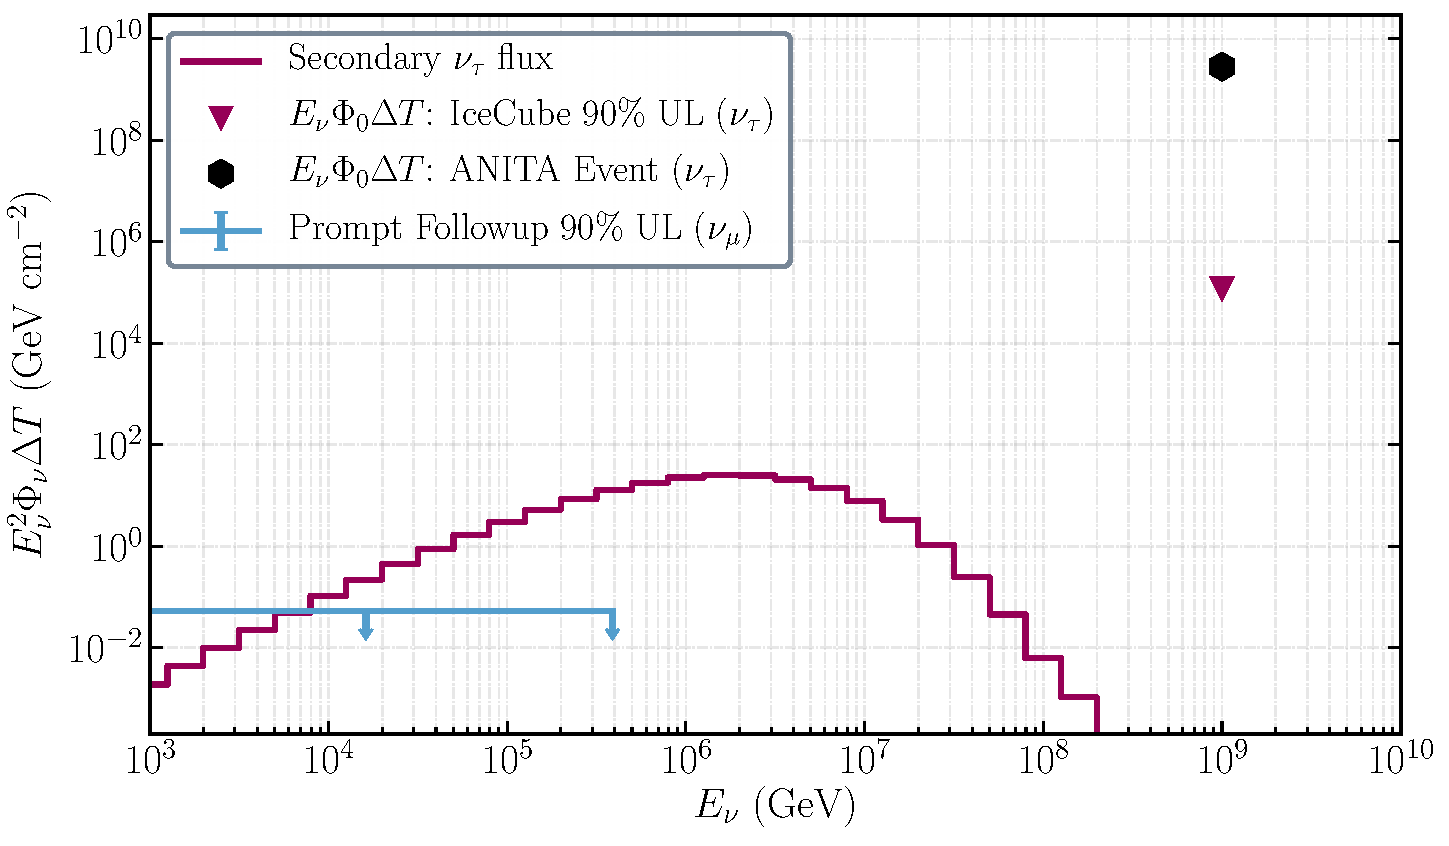
\includegraphics[width=0.65\textwidth]{figures/ANITA/ANITA_pspaper_secondaries_NOpreliminary_deltaT.pdf}
  \label{fig:ANITA_taurunner_limits}
  \caption[ANITA secondary fluxes]{Upper limits (90\% C.L.) placed by calculating the secondary neutrino flux (purple histogram) from an incident flux of EeV neutrinos assuming constant emission over $10^3$ s and comparing to the nonobservation of IceCube events in the prompt analysis described in Sect.~\ref{ref:subsec:ANITA_prompt} for AAE-141220. The flux implied by the ANITA observations (black), represented in this figure as $E_{\nu}\Phi_0 \Delta T = E_{\nu} \Delta T \int \Phi(E_{\nu}, t) \diff E_{\nu}$, using information about ANITA's acceptance \citep{Romero-Wolf:2018zxt} overshoots this upper limit (purple arrow) by many orders of magnitude. For comparison, upper limits on the time-integrated muon-neutrino flux from the prompt analysis are shown in blue. All fluxes are per flavor $\nu + \bar{\nu}$.}
\end{figure*}

The method presented here, constraining high-energy fluxes by looking for secondaries, has a wide range of applications. For example, this method could be beneficial for future correlation searches with radio detectors and future Cherenkov detectors such as POEMMA \citep{Venters:2019xwi}, for point source searches from extreme transients \citep{Righi:2020ufi}, or for searches of GZK neutrinos.


 %DONE

\part{Bringing Multi-Messenger Astronomy to the Public}
\chapter{DECO: the Distributed Electronic Cosmic-Ray Observatory}
\label{sec:DECO}
\chapter{Multi-messenger astronomy: the Universe through neutrino colored glasses}
\label{chapter:public}
\chapter{Astrobites}

\appendix
\chapter{Seasonal variation of atmospheric neutrino event rates}
\label{sec:seasonal}

Proper modeling of background data (especially with respect to time) is tantamount to successful short timescale analyses. Although to first order, background distributions seem independent of time, there is known underlying oscillatory structure at the $\mathcal{O}(10\%)$ level due to changes in atmospheric conditions, which affect atmospheric lepton production rates from cosmic-ray interactions. Many current analyses do not take this \textit{seasonal variation} into account, and those that do have treated the rate as a one-dimensional sine wave in time affecting the rate of the entire sample. Here, we investigate if this is a proper treatment. 

We begin with the assumption that we are working with a finite viewing window of a sinusoidal rate, $\mathcal{R}$\footnote{here, $\mathcal{R}$ is only the fluctuation from the mean rate, $\mathcal{R} = \frac{r-<r>}{<r>}$, where $r$ is the true rate}:

\begin{equation}
\label{eq:rate}
    \mathcal{R}(f,t,\delta, w) = \Pi \left(\frac{t-\pi  w}{2 \pi  w}\right) \sin (2 \pi  \delta +f t) \; , 
\end{equation}

where $t$ is the time, $f$ is the frequency, $\delta$ is an offset, and our viewing window is encompassed by a unit step function, $\Pi$, with width characterized by $w$. 

We are interested in observing this rate in frequency space, and naturally wish to take a Fourier Transform (FT). We will apply this procedure to our rate as a function of time, but also try to account for structures that should manifest in the FT from known imperfections in these data. In general, the FT of a function of time is given by

\begin{equation}
\label{eq:FFT}
    \mathcal{F}_t[\mathcal{R}(t)](\omega ) = \frac{1}{\sqrt{2 \pi}} \int_{-\infty}^{\infty} \mathcal{R}(t) e^{i \omega t} d t \; .
\end{equation}

We know that in the case of a pure sinusoid, the $\mathcal{F}$ operator should return delta functions corresponding to the frequency of our rate. This is also the case for an infinite viewing window,

\begin{equation}
    \lim_{w\rightarrow \infty} \mathcal{F}_t[\mathcal{R}(t)](\omega ) = i \sqrt{\frac{\pi }{2}} e^{-2 i \pi  \delta } \delta (\omega -f)-i \sqrt{\frac{\pi }{2}} e^{2
   i \pi  \delta } \delta (f+\omega ) \; .
\end{equation}

One immediate problem is that we have limited years of data, so we begin by investigating the effect that a limited viewing window has on our FT. Applying Eq.~\ref{eq:FFT} to our rate function defined in Eq.~\ref{eq:rate}, and taking the magnitude in $\mathbb{C}$, we get 

\begin{multline}
   \mathcal{F}_t[\mathcal{R}(t)](\omega ) =  \Bigg| \frac{1}{4\pi (f^2 - \omega^2)}(\theta (-w)-\theta (w)) (\cos (2 \pi  (\delta +f w-w \omega ))-i \sin (2 \pi  (\delta +f w-w
   \omega ))) \; \times \\ \qquad (2 i (f-\omega ) \sin (\pi  w (f+\omega )) (\cos (4 \pi  \delta +3 \pi  f w-\pi
    w \omega )+i \sin (4 \pi  \delta +3 \pi  f w-\pi  w \omega )) \; +  \\ (-f-\omega ) (i \sin (2 \pi
    f w-2 \pi  w \omega )+\cos (2 \pi  f w-2 \pi  w \omega )-1)) \Bigg| \; ,
\end{multline}

which can be simplified to 

\begin{multline}
    \mathcal{F}_t[\mathcal{R}(t)](\omega ) = \frac{1}{4\pi} \Big| \frac{1}{f^2 - \omega^2} \Big( e^{- 2 \pi i (fw+\delta-w\omega)}\big(-(f+\omega)(-1+e^{2\pi i w(f-\omega)}) + \\ 2i\sin (\pi w(f + \omega)) e^{i(3f\pi w + 4\pi \delta - \pi w \omega)}\big) \Big) \Big|
\end{multline}

A sample time series and the corresponding FT are displayed in Fig.~\ref{fig:ex_fft}. Here, the effect of the finite viewing window is visible in the separate peaks in the FT, a consequence often referred to as \textit{spectral leakage}\footnote{For a thorough writeup on spectral leakage, see \url{https://en.wikipedia.org/wiki/Spectral_leakage}.}.
\begin{figure}
    \centering
    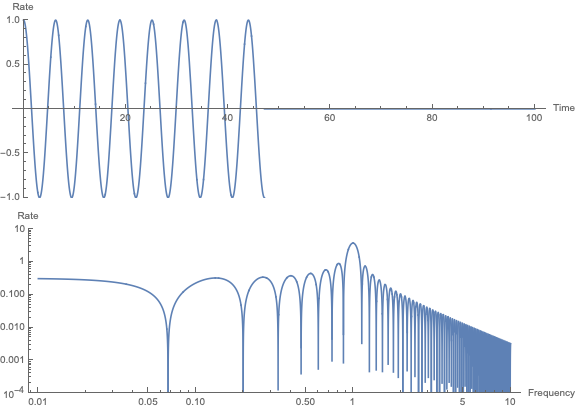
\includegraphics[width=0.90\textwidth]{figures/seasonal/box_fft_sample.png}
    \caption[Windowing effect in FFTs]{A sample time series (top) with a pure sine wave and finite viewing period (7.5 cycles) with corresponding FT (bottom)}
    \label{fig:ex_fft}
\end{figure}
%In the gamma-ray followup (GFU) dataset, it has been noted in the past that the effects of seasonal variations are evident, and manifest in an overall $\mathcal{O}$(10\%) fluctuation in the background rate. 
%For short timescale analyses, an accurate prediction of the background rate is of utmost importance in quantifying the significance of a possible signal. As a result of seasonal variations, calculating the rate from the entire livetime of the dataset leads to systematic over- and under-estimations of the rate, whereas parameterizing the background rate from data around the time of a transient event is limited by statistical fluctuations of the rate. In order to see if we can model the rate as a sinusoid, we take an FFT of the rate data, and try to make sure that any features can be explained by what is expected from an FFT of a windowed sinusoid.

\begin{figure}
    \centering
    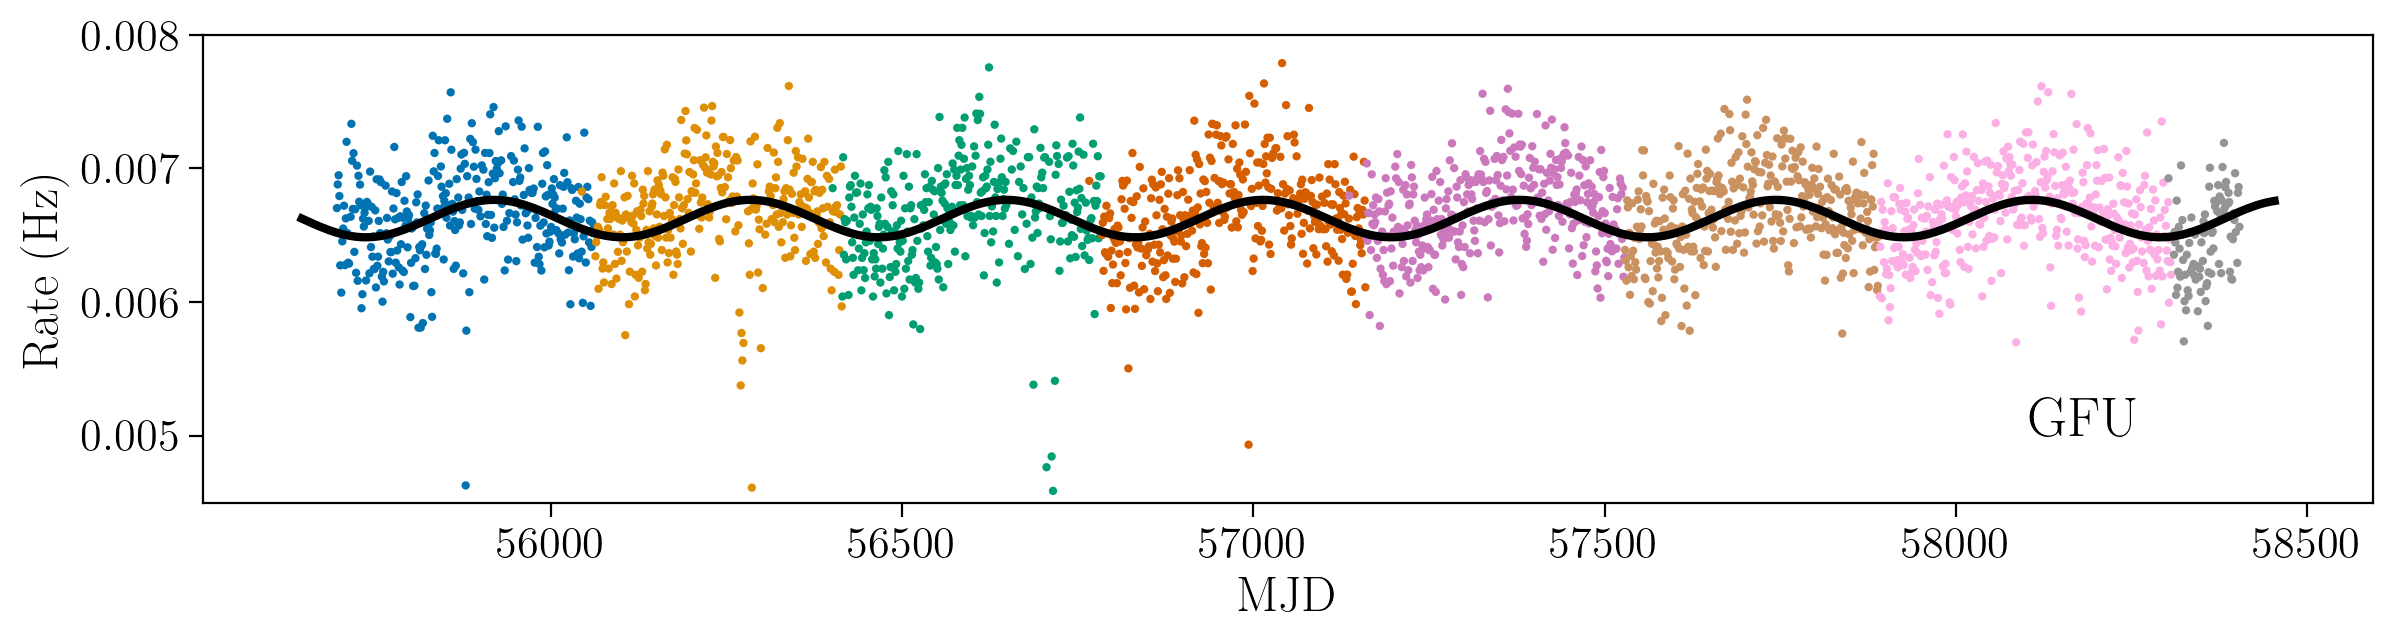
\includegraphics[width=0.9\textwidth]{figures/seasonal/gfu_online_overall_with_model.png}
    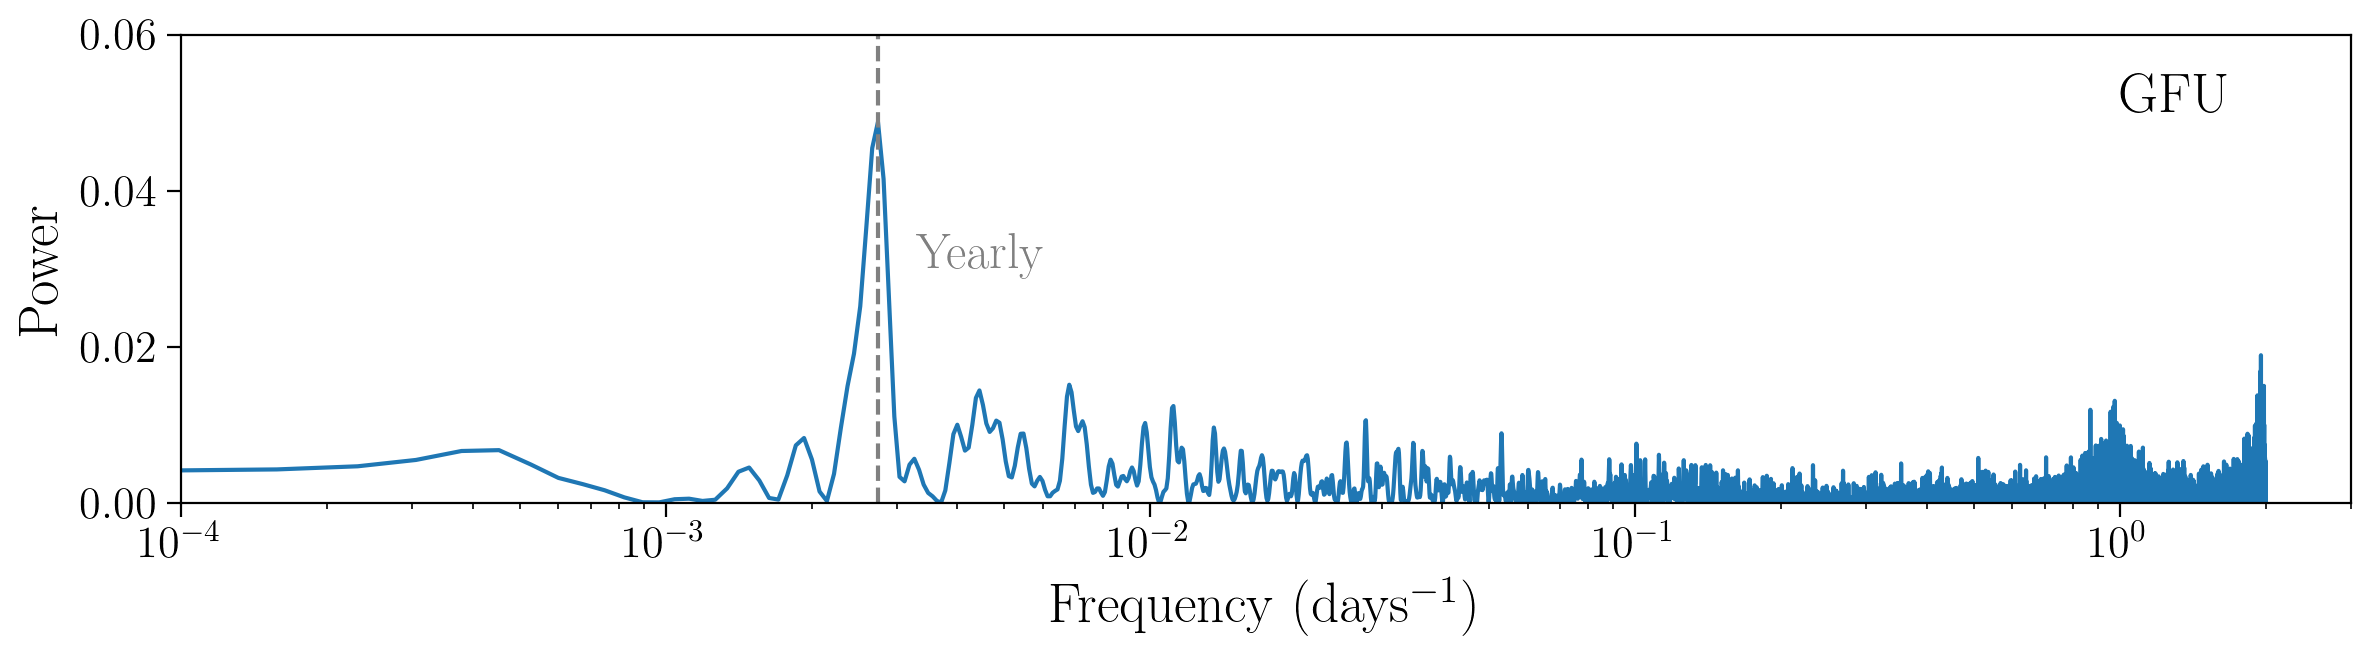
\includegraphics[width=0.9\textwidth]{figures/seasonal/gfu_online_overall_FFT_maxima_False.png}
    \caption[GFU all sky rate]{GFU time series (top) and FT (bottom) for 7.5 years of data. Each color is a different season of IC86 data.}
    \label{fig:gfu_7_year_fft}
\end{figure}

Fig.~\ref{fig:gfu_7_year_fft} shows the rate time series and corresponding FT for the 7.5 years of available data from GFU. Here, as the data is sampled unevenly, we use the Lomb-Scargle periodogram\footnote{For details on the algorithm, see \url{https://arxiv.org/abs/1703.09824}.} algorithm to transform these data into frequency space. There is clear structure to the left of the annual peak. To investigate if these are the expected peaks, we extremize numerically, and find that there should be peaks at frequencies of $\{0.41,0.54,0.67,0.8\}\times f_0$, where $f_0$ is the peak frequency in the plots in the figures above. The numerical derivative has some odd structure, and is displayed in Fig.~\ref{fig:fft_derivative}.

\begin{figure}
    \centering
    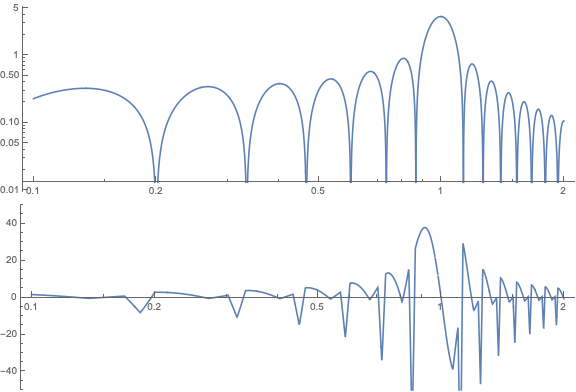
\includegraphics[width=0.75\textwidth]{figures/seasonal/GFU_fft_with_derivative.png}
    \caption[Numerical derivative of FFT of windowed data]{FT (top) and numerical derivative of FT (bottom)}
    \label{fig:fft_derivative}
\end{figure}

Looking at other durations and doing a crude fit, it seems as though the maxima appear at roughly $f_0 + (\frac{3}{2} + n)\frac{1}{w}$, where $n = 0,1,2,\ldots$
Placing lines at the corresponding frequencies in the GFU FT results in Fig.~\ref{fig:gfu_with_harmonics}

\begin{figure}
    \centering
    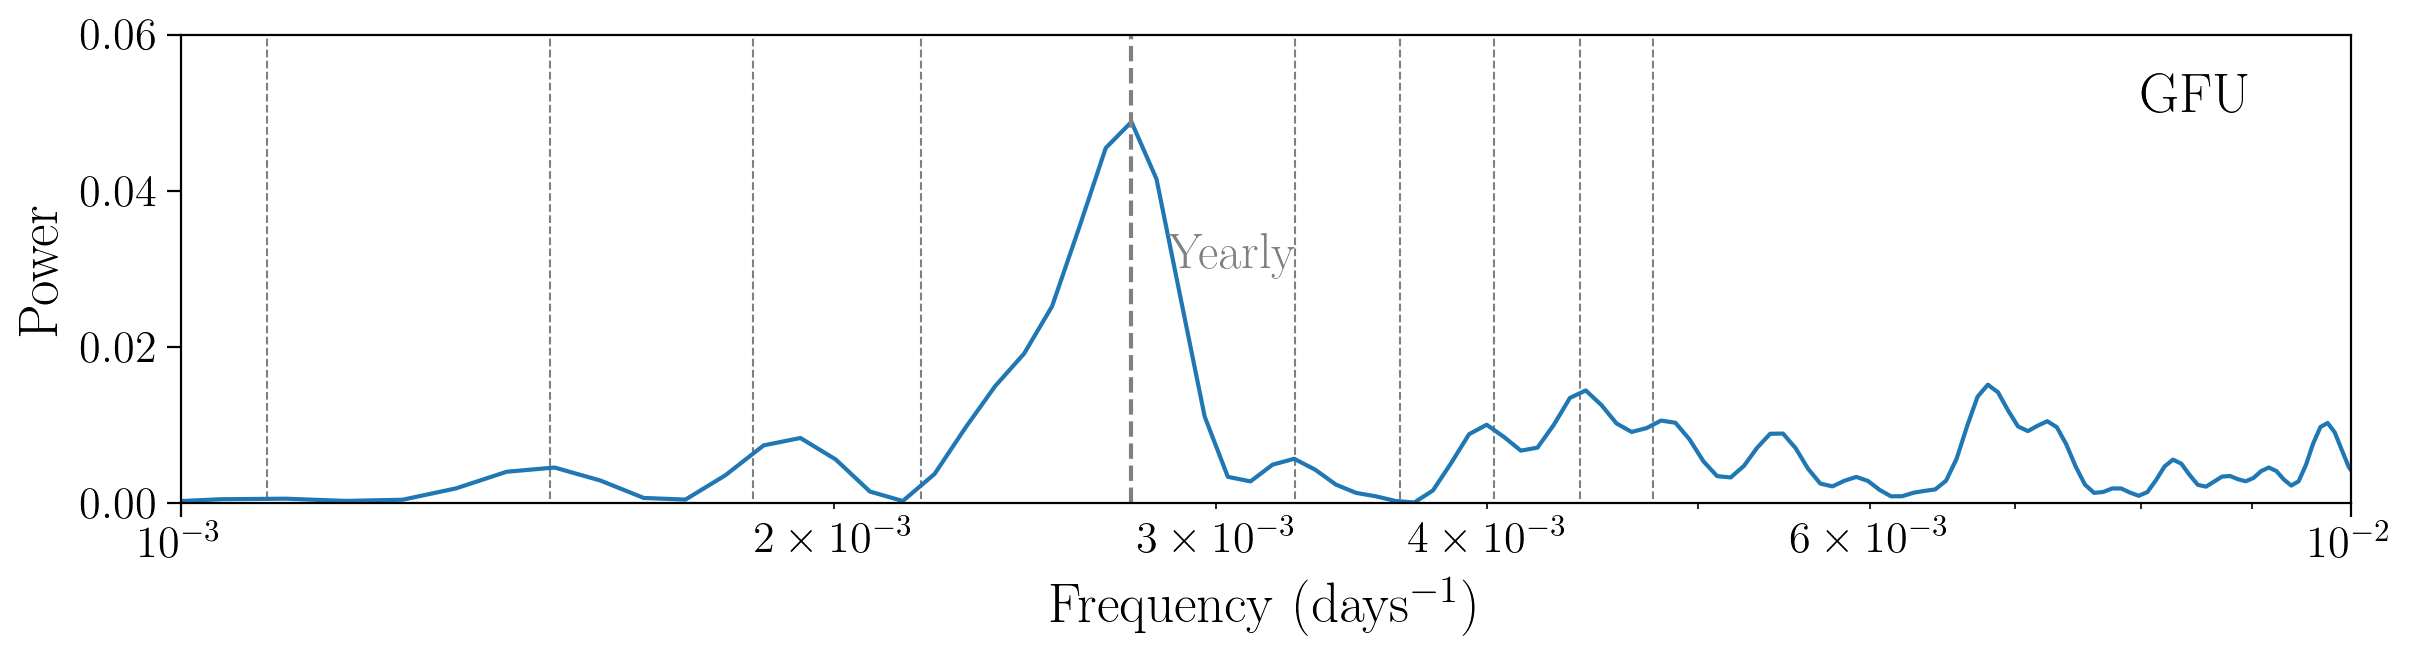
\includegraphics[width=0.95\textwidth]{figures/seasonal/gfu_online_overall_FFT_maxima_True.png}
    \caption[FFT numerical derivative]{GFU FT with additional lines at the locations of the extremal frequencies extracted from Fig.~\ref{fig:fft_derivative}}.
    \label{fig:gfu_with_harmonics}
\end{figure}

\section{Declination Dependence}
Seasonal variations are mainly a function of atmospheric properties. As the temperature and pressure of the atmosphere fluctuate, the ratio of the decay length to interaction length for $\pi^{\pm}$ created from cosmic-ray interactions will vary. As such, the the magnitude of the seasonal variation effect is dependent on zenith angle, $\theta$ (plots shown here are for Equatorial coordinates shown in slices of equal solid angle, or equal $\sin \delta$). 

We begin by repeating the procedure of the previous section, but in various declination bands. The result is shown in Fig.~\ref{fig:dec_bands}.

\begin{figure}
    \centering
    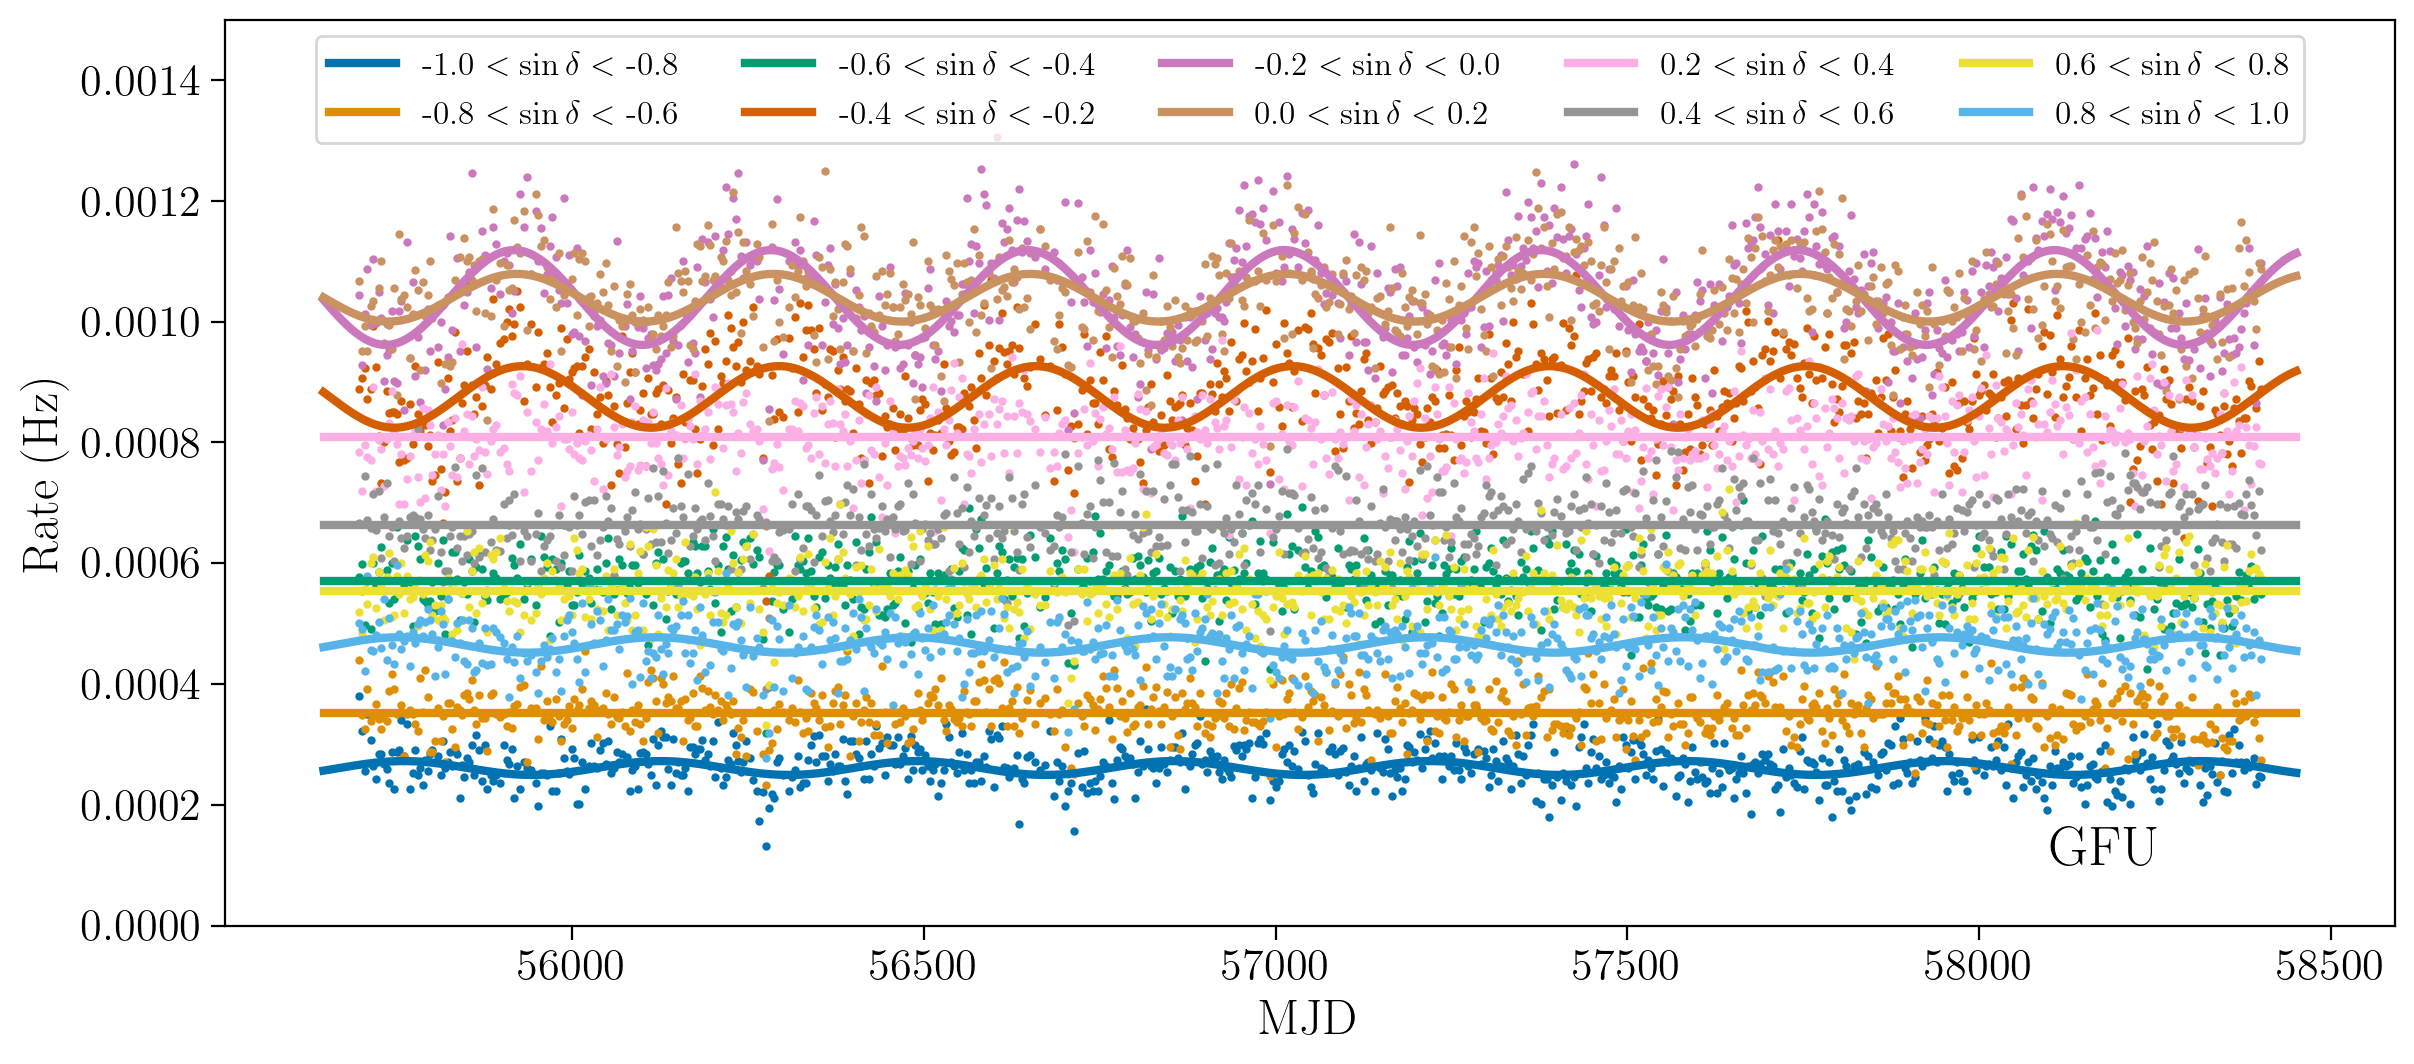
\includegraphics[width=0.99\textwidth]{figures/seasonal/gfu_online_dec_band_with_model.png}
    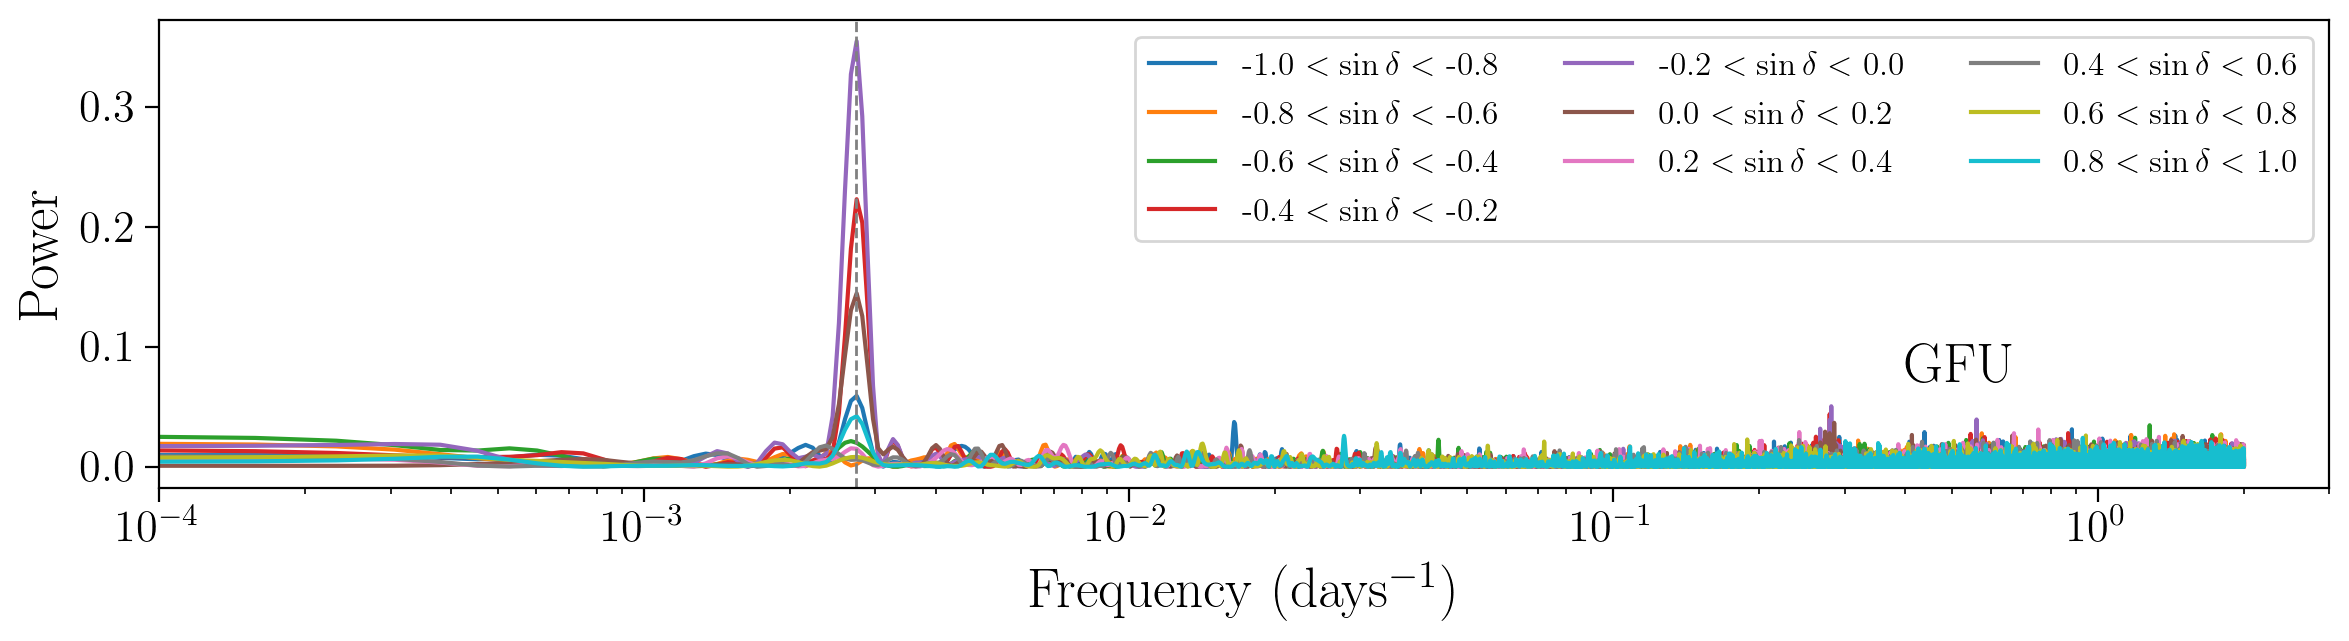
\includegraphics[width=0.99\textwidth]{figures/seasonal/gfu_online_dec_bands_FFT.png}
    \caption[\texttt{GFU} seasonal variations]{Rate as a function of time for various declination bands (top). Fits are only included if the p-value of the annual structure in the FT is at or below the 1\% level. FT (bottom) highlights that seasonal variations are more evident in certain declination bands}
    \label{fig:dec_bands}
\end{figure}

Although seasonal variations are expected in all samples, the magnitude of the effect varies from sample to sample, depending on how contaminated the sample is with atmopherics. See for example by comparing the frequency dependence of the GFU sample to that of the ps-tracks sample, which is shown in Fig.~\ref{fig:dec_bands_ps_tracks}.

\begin{figure}
    \centering
    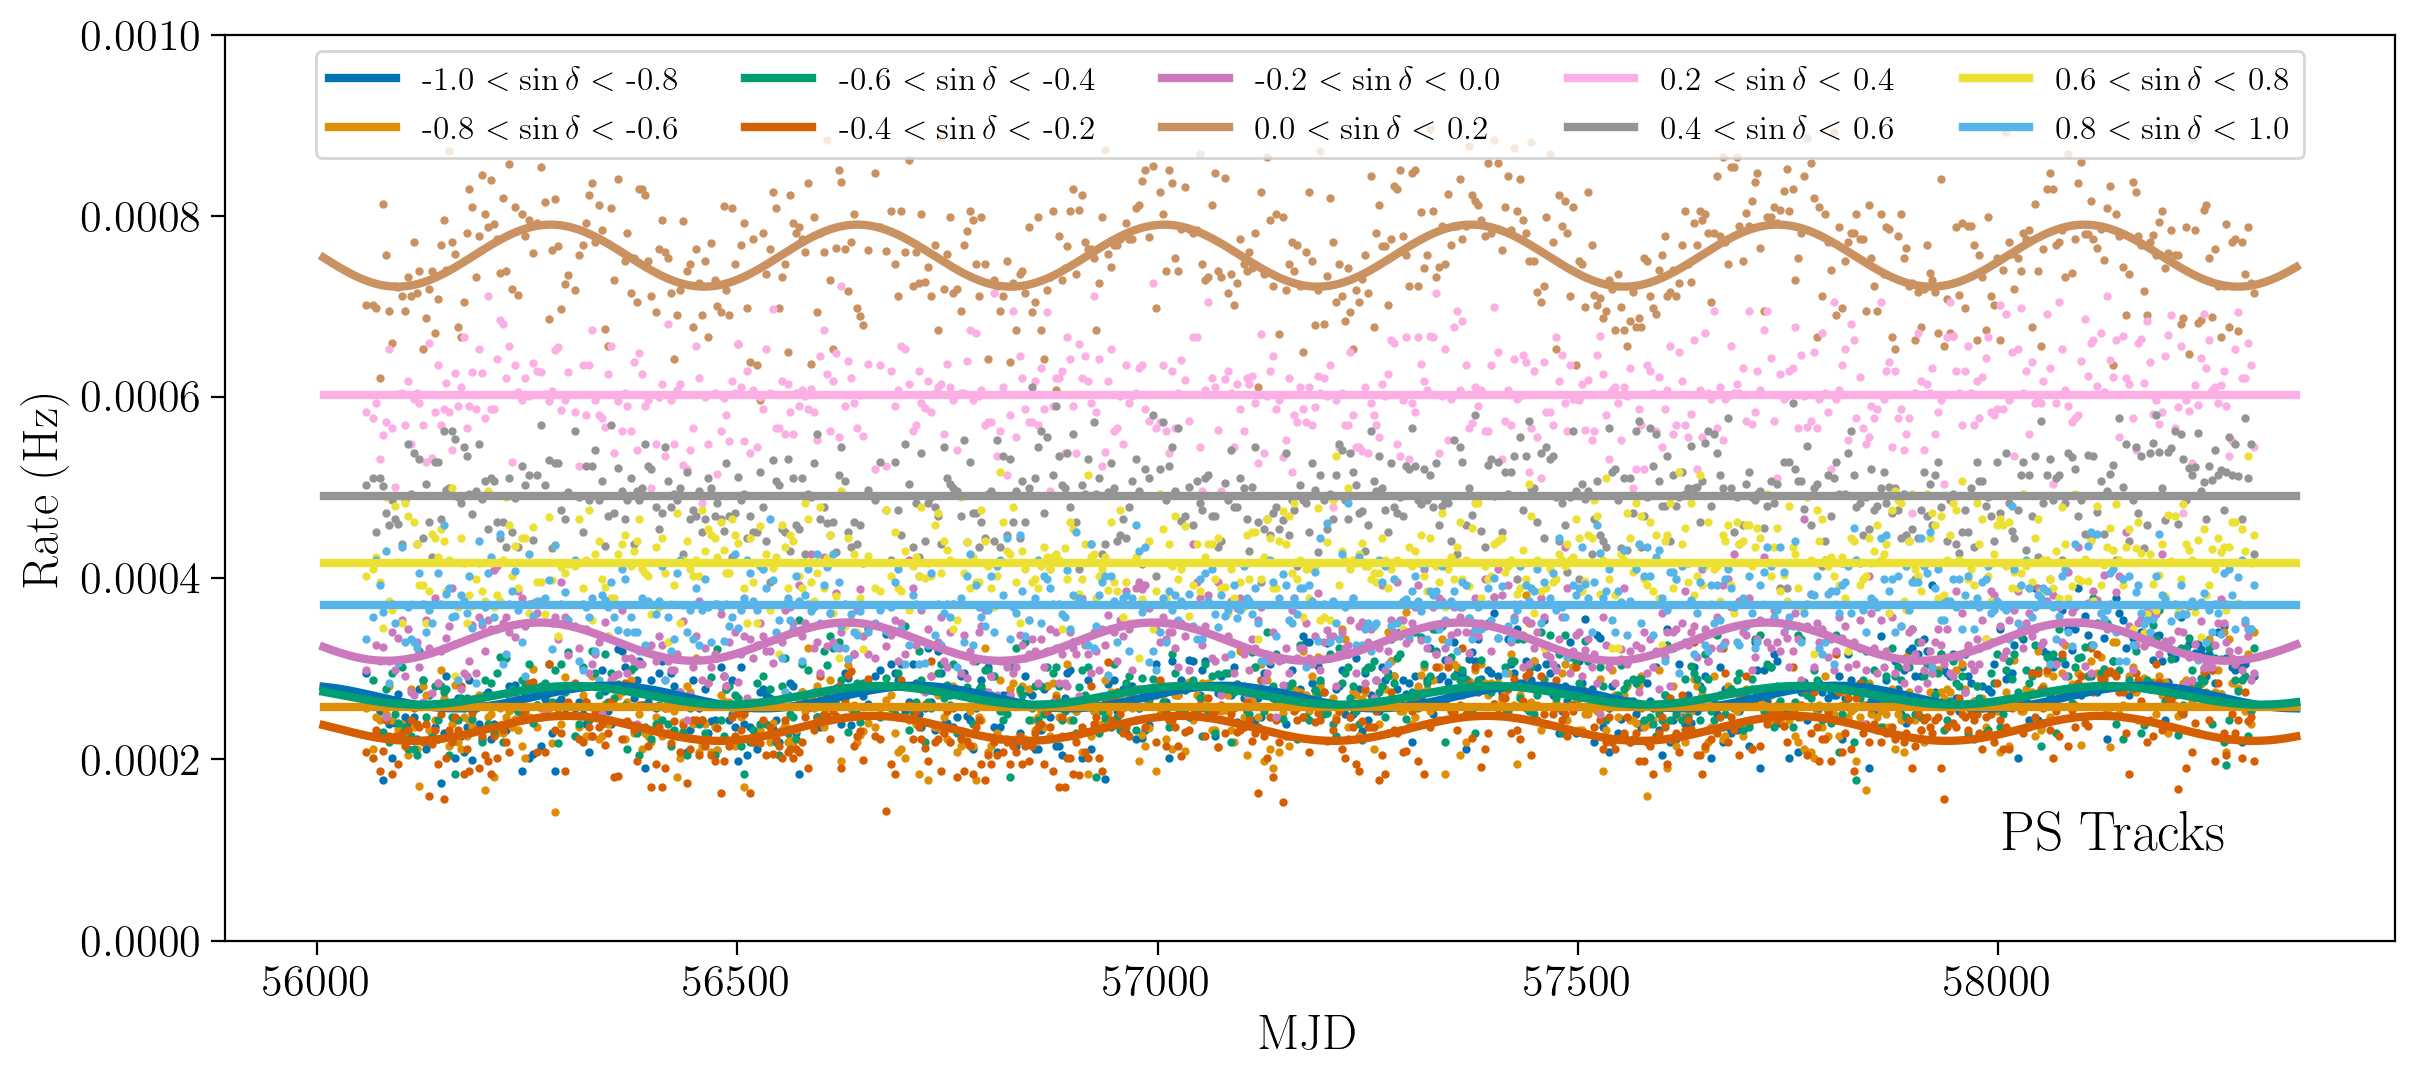
\includegraphics[width=0.99\textwidth]{figures/seasonal/ps_tracks_dec_band_with_model.png}
    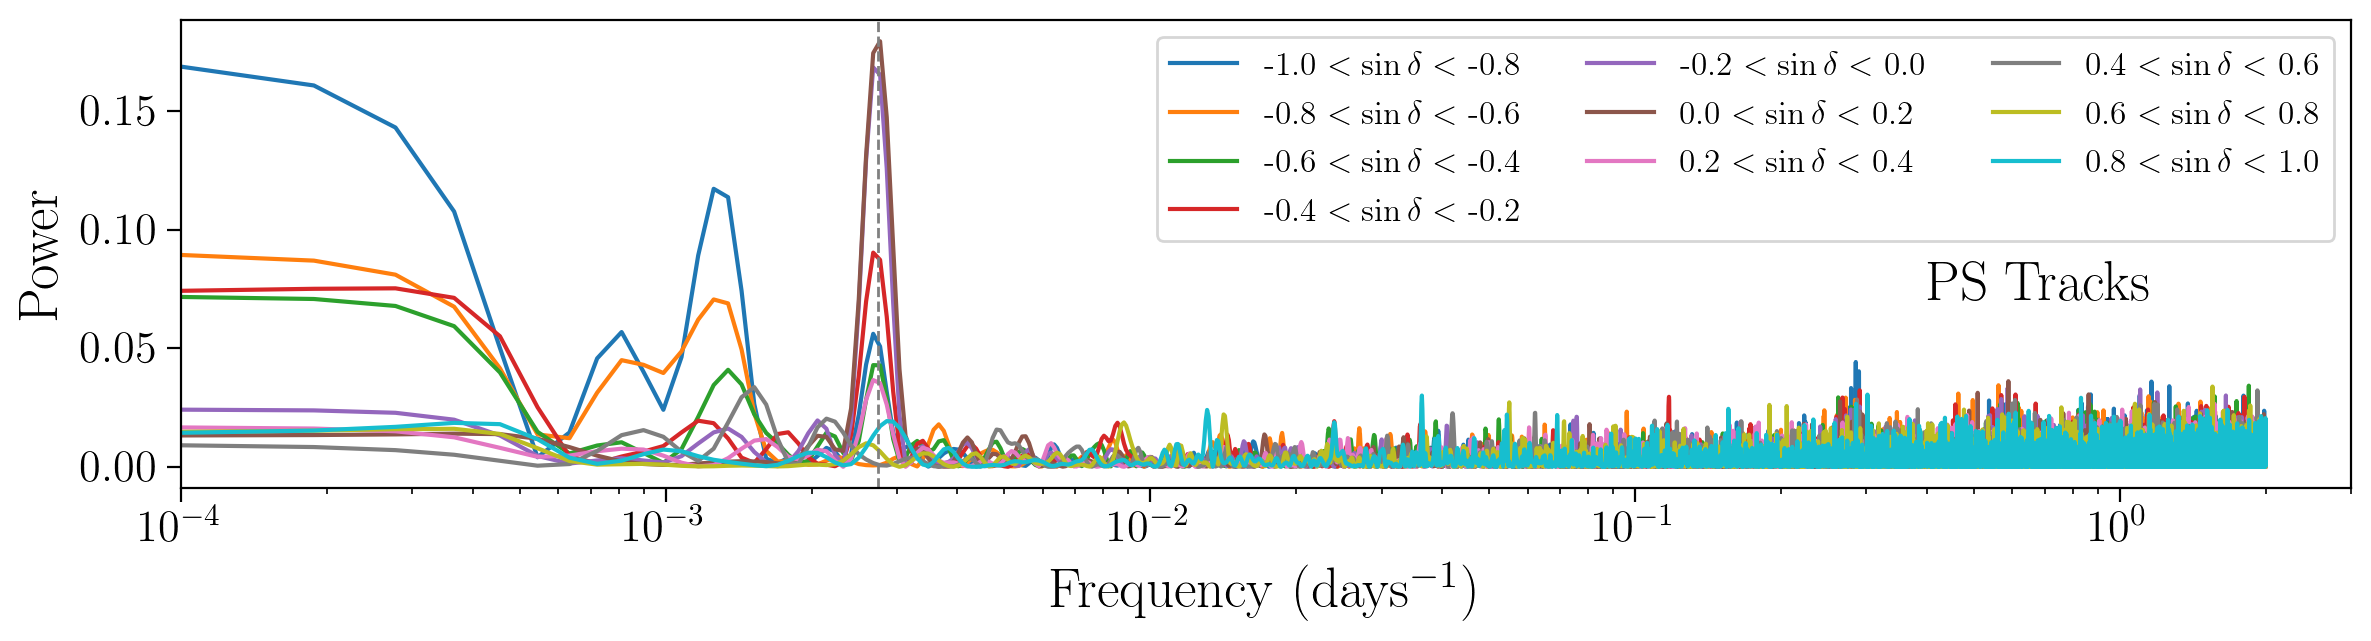
\includegraphics[width=0.99\textwidth]{figures/seasonal/ps_tracks_dec_bands_FFT.png}
    \caption[\texttt{ps-tracks} seasonal variations]{The same as Fig.~\ref{fig:dec_bands} but for the \texttt{ps-tracks} sample.}
    \label{fig:dec_bands_ps_tracks}
\end{figure}

Instead of looking at the FTs in terms of the power in each frequency, one can also look at the amplitude (in units of the rate, and thus not normalized to the rate in each declination band). We display these as vectors in a 2D plane for both event selections, shown in Fig.~\ref{fig:phasor}. 

\begin{figure}
    \centering
    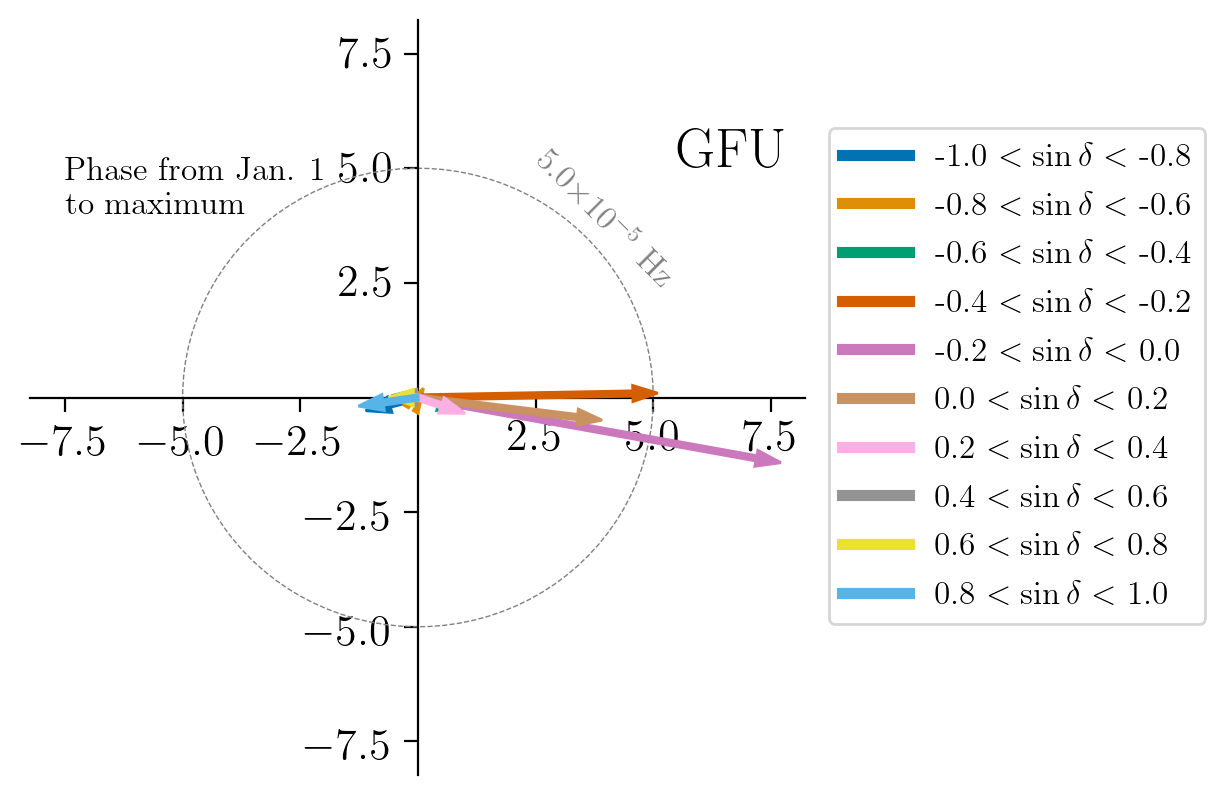
\includegraphics[width=0.48\textwidth]{figures/seasonal/gfu_online_phasor.png}
    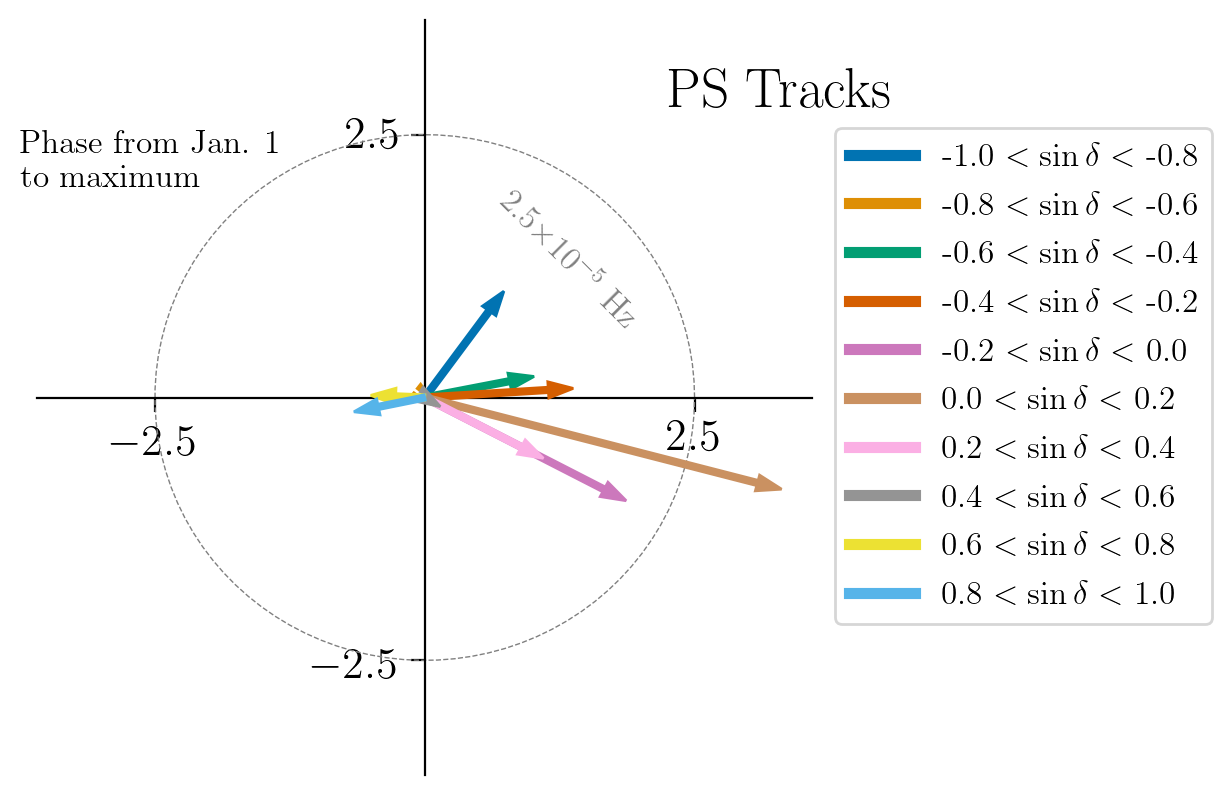
\includegraphics[width=0.48\textwidth]{figures/seasonal/ps_tracks_phasor.png}
    \caption[Seasonal variation phasors]{Phases and amplitudes of the annual peak in the FT broken down by declination band. For different zenith angle bands, the phases of the sinusoids are out of phase, in some cases nearly 180$\deg$. }
    \label{fig:phasor}
\end{figure}

Phases in Fig.~\ref{fig:phasor} are shown as the phase from Jan. 1 to the phase of maximal amplitude, as shown by the schematic in Fig.~\ref{fig:ft_schematic}. 

\begin{figure}
    \centering
    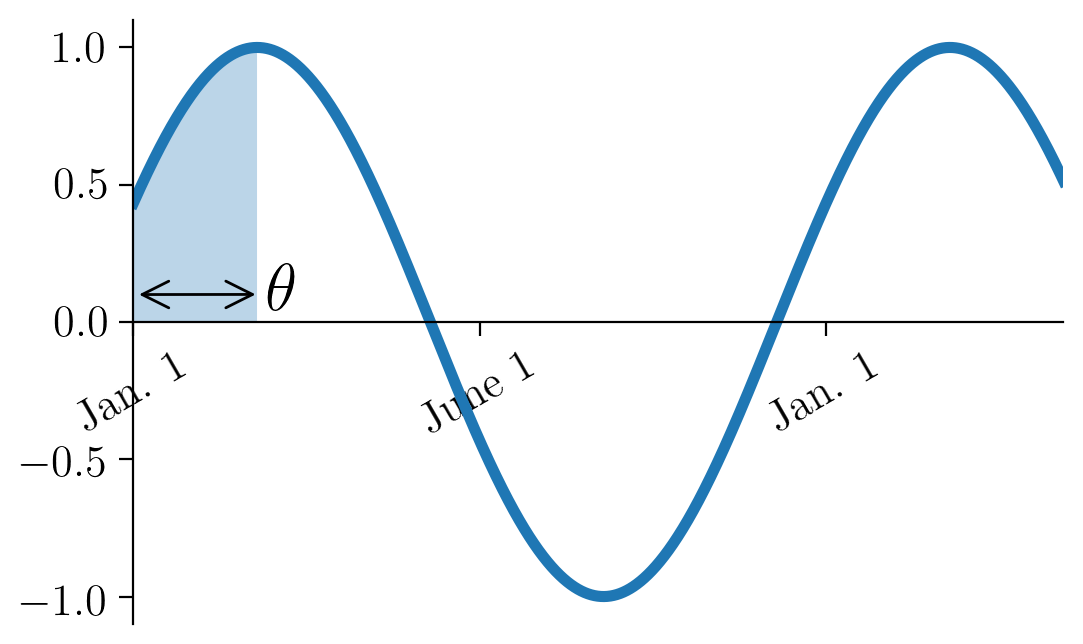
\includegraphics[width=0.55\textwidth]{figures/seasonal/phase_schematic.png}
    \caption[Phase convention schematic]{Definition of the phases for Fig.~\ref{fig:phasor}.}
    \label{fig:ft_schematic}
\end{figure}

As both the relative and absolute magnitudes, as well as the phase information, are important, we plot all three as a function of declination, here only focusing on the GFU dataset. The result is shown in Figure~\ref{fig:seasonal_3panel}. 

\begin{figure}
    \centering
    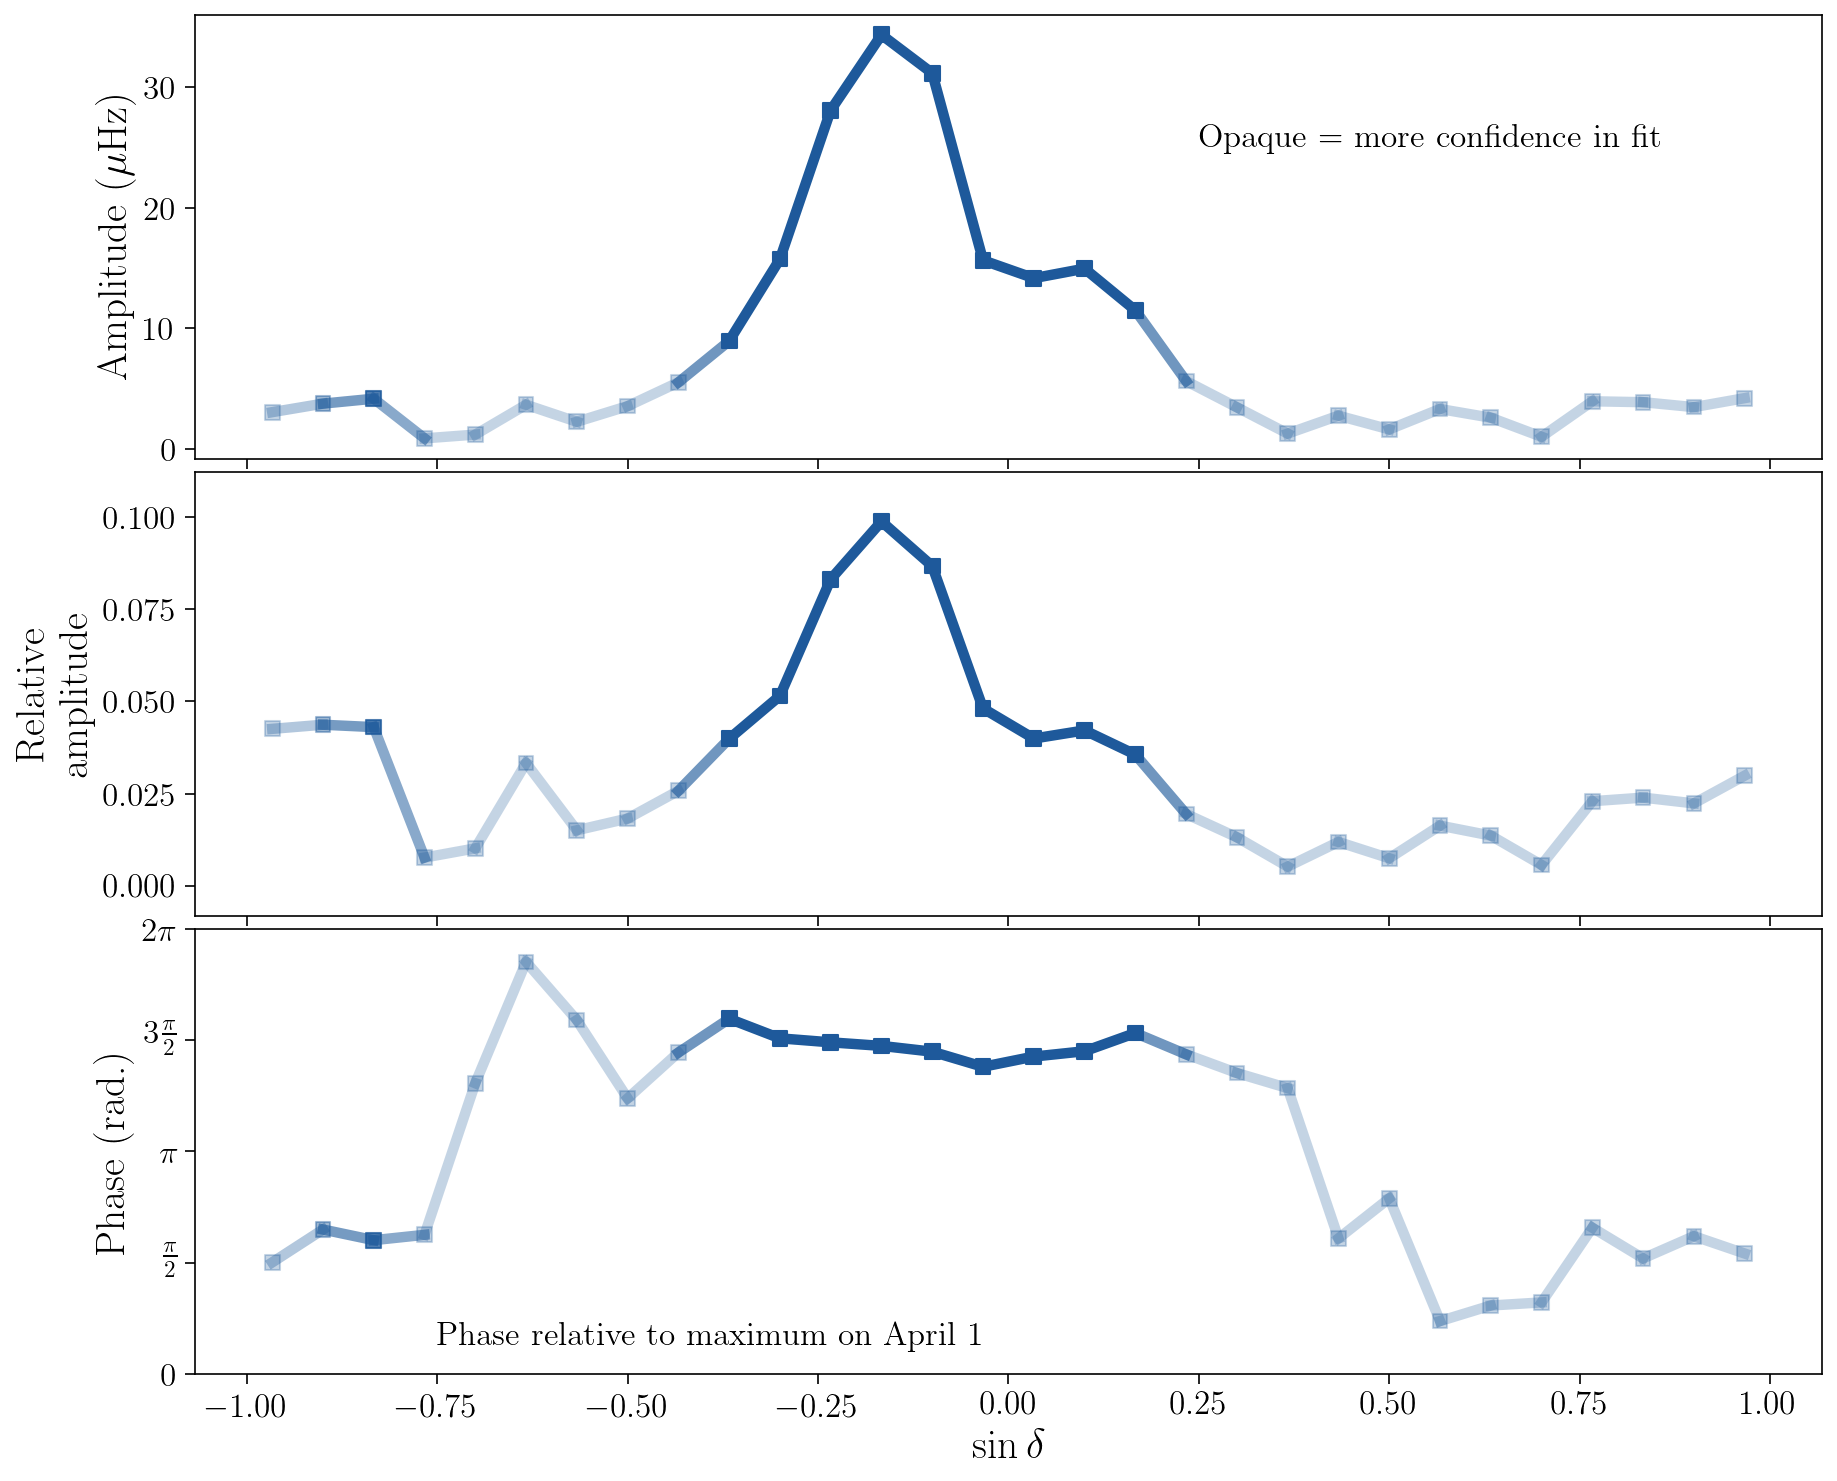
\includegraphics[width=0.95\textwidth]{figures/seasonal/seasonal_3panel_plot.png}
    \caption[Absolute and relative fourier component magnitudes]{Evolution of the absolute magnitude (top), relative magnitude (middle), and phase (bottom) of the annual sinusoidal component in the GFU event sample rate. Data points that appear transparent are regions where the sinusoidal fit was not preferred strongly over a constant rate. Regardless, the amplitudes still display a clear pattern as a function of declination, peaking near the horizon as one would expect.}
    \label{fig:seasonal_3panel}
\end{figure}

Although in some declination bands, the sinusoidal component is not dominant enough to be fit confidently, there is still a clear trend in the effect as a function of declination.  %DONE
\chapter{Fast Response Analysis Tutorial}
\label{sec:FRA_tutorial}

Here I provide a brief overview on how to use the Fast Response Analysis (FRA) pipeline. The code is available at \url{https://github.com/IceCubeOpenSource/FastResponseAnalysis}, and a similar walkthrough appears in the \texttt{README} of this repository. 

\subsection{Installation}
The FRA code has a dependency on the IceCube realtime software. This enables the user to query the realtime database and access events detected at Pole with a latency of around 30 seconds. The trunk (and any release including and after v02-00) use python3. v01-00 uses python2, and as such, if you would like to use that version, you may have to adjust the installation below to point to relevant python2 environments. To set up the IceCube realtime software, perform the following commands:

\begin{lstlisting}[language=bash]
eval `/cvmfs/icecube.opensciencegrid.org/py3-v4.1.0/setup.sh`
svn co http://code.icecube.wisc.edu/svn/meta-projects/combo/releases/V01-00-00/ src
mkdir build 
cd build
cmake ../src
make
\end{lstlisting}

After you have a version of icerec built, you will want to do a parasitic build of the realtime project, building off of this version of icerec. To do this, navigate to a new directory where you want your realtime project to live, and run

\begin{lstlisting}[language=bash]
svn co http://code.icecube.wisc.edu/svn/meta-projects/realtime/trunk/ src
mkdir build 
cd build
cmake ../src/ -DMETAPROJECT=/path/to/icerec/build/ -DCMAKE_INSTALL_PREFIX=combo-plus.${OS_ARCH}
make
\end{lstlisting}

You can now load the realtime project with

\begin{lstlisting}[language=bash]
/path/to/realtime/build/env-shell.sh
\end{lstlisting}

Once you are in your realtime project, you will need to install the relevant dependencies this project requires. We recommend making a virtual environment and installing the relevant dependencies by running the following lines

\begin{lstlisting}[language=bash]
python3 -m venv fra_env
source fra_env/bin/activate
pip install -r /path/to/fast-response/requirements.txt
\end{lstlisting}

% This will create a virtual environment names \texttt{fra_env}, and the source \texttt{fra_env/bin/activate} line will activate the environment.

In the future, you will not need to jump through these hoops, and you can load the environment with these lines:

\begin{lstlisting}[language=bash]
eval `/cvmfs/icecube.opensciencegrid.org/py3-v4.1.0/setup.sh`
/path/to/realtime/build/env-shell.sh
source /path/to/fra_env/bin/activate
\end{lstlisting}

If you would like to be able to import fast response tools from any directory in the future, you must append to your python path with

\begin{lstlisting}[language=bash]
export PYTHONPATH=$PYTHONPATH:/path/to/fast-response
\end{lstlisting} 
\chapter{Visualizing the neutrino source density and luminosity parameter space}
\label{sec:density_lumi_rotate}

With the measurement of a diffuse neutrino flux but uncertainties in the astrophysical origins, one can ask if the dominant source class which produces neutrinos are \textit{rare and bright} or \textit{numerous and dim}. One way to do this is by looking for point source excesses. With the lack of any clear point sources, neutrino bright objects can be excluded, and thus attributing the entire diffuse flux from steady, rare ($<\mathcal{O}(1\; \mathrm{Gpc}^{-3})$) objects can be excluded with current limits. The effective source densities which can be probed change significantly with a detector like Gen2. All of this is normally visualized in Figure~\ref{fig:rotate_current_fig} (Figure taken from \cite{Aartsen:2019swn}).

\begin{figure}[h!]
    \centering
    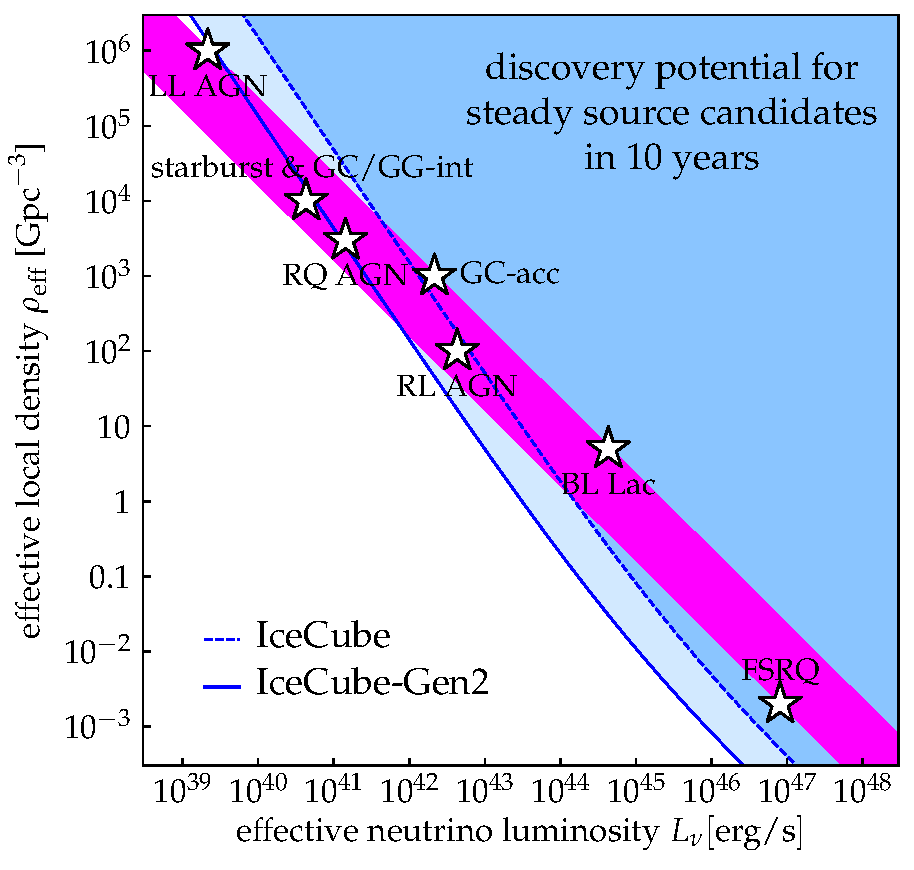
\includegraphics[width=0.45\textwidth]{figures/rotated_phase_space/continuous_Gen2_revised.pdf}
    \caption[Original density luminosity plane]{Comparison of the diffuse neutrino flux (magenta) to current and projected point source sensitivities (blue lines), as well as the effective local source density and luminosity of various candidate source classes.}
    \label{fig:rotate_current_fig}
\end{figure}

A quick notes about the figure: making an argument such as ``x\% of source class y could still explain the diffuse flux'' is true if the star corresponding to source class y, when moved down on the y-axis by the appropriate ratio, is below the point source limits.

This way of visualizing the parameter space downplays the large region of parameter space the Gen2 could probe. Also, it is the transpose of what you might intuitively do, as luminosity is somewhat analagous to flux, which we plot vertically and forbid regions above (not to the right of) limits. Additionally, even under the assumption that numerous source classes contribute to the diffuse flux, there are likely only one or a few that contribute at a greater than 10\% level, and these are the real targets of searches in this spirit. As a result, the true parameter space of interest is not as large as this plot would lead you to believe. 

Some suggestions for improvement include transposing the plot and possibly hatching the part of the parameter space that explains 100\% of the diffuse flux once we have gen2, as is pictured in Figure~\ref{fig:rotate_transposed}.

\begin{figure}[htb]
    \centering
    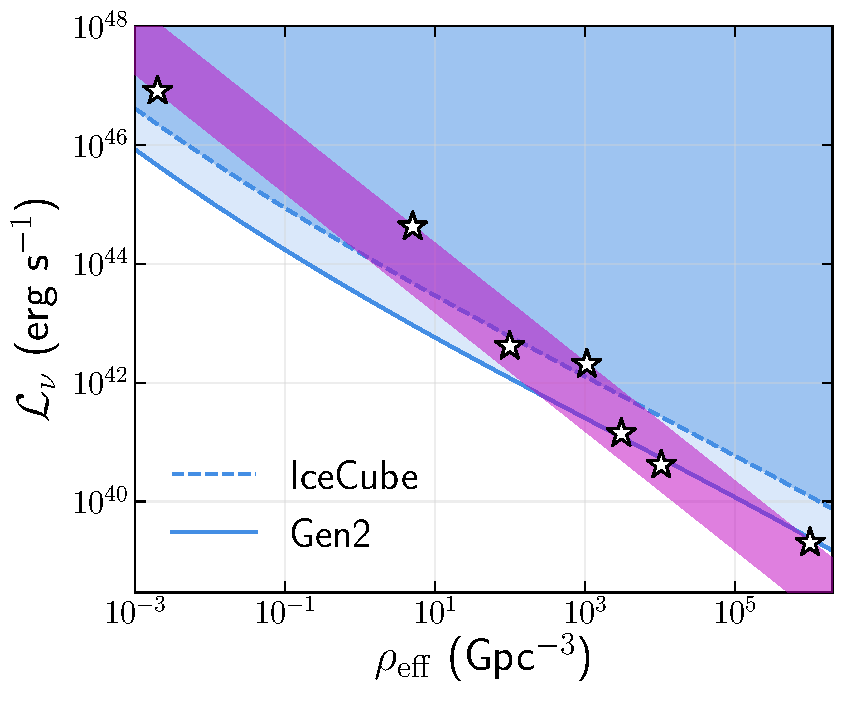
\includegraphics[width=0.48\textwidth]{figures/rotated_phase_space/lumi_density_rotated.pdf}
    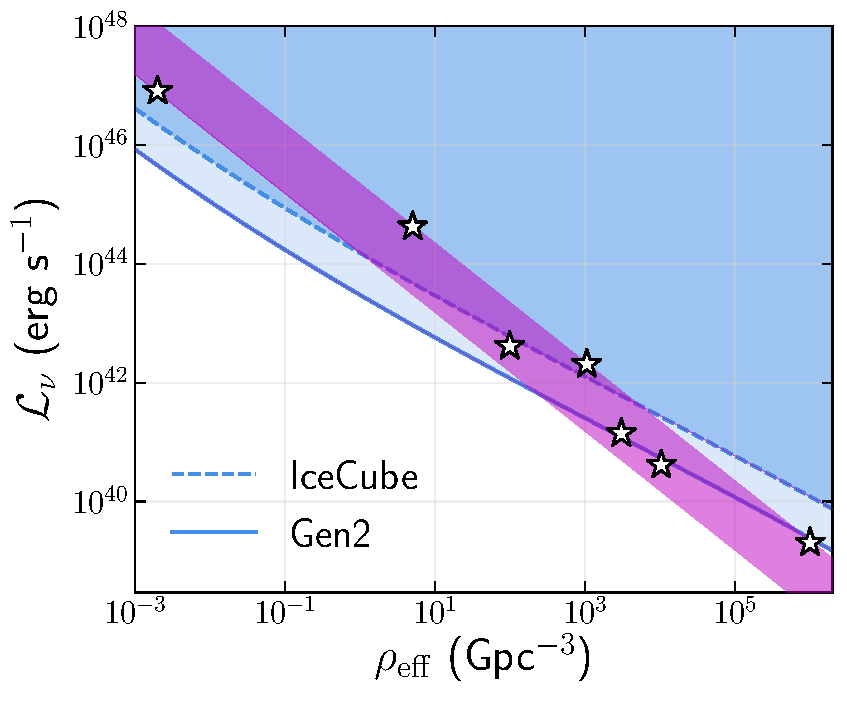
\includegraphics[width=0.48\textwidth]{figures/rotated_phase_space/lumi_density_hatched_rotated.pdf}
    \caption[Transpose of luminosity density plane]{Transpose of the previous figure, so that higher luminosities are found by moving vertically upwards in the plot}
    \label{fig:rotate_transposed}
\end{figure}

This plot still has the problem of presenting a lot of uninteresting phase space (bottom left). To remedy this, we could plot $\rho_{eff}\times \mathcal{L}_{\nu}$ on the vertical axis, in much the same way that power law spectra are scaled by powers of $E_{\nu}$. Doing this results in Figure~\ref{fig:rotate_scaled_lumi_density}.

\begin{figure}
    \centering
    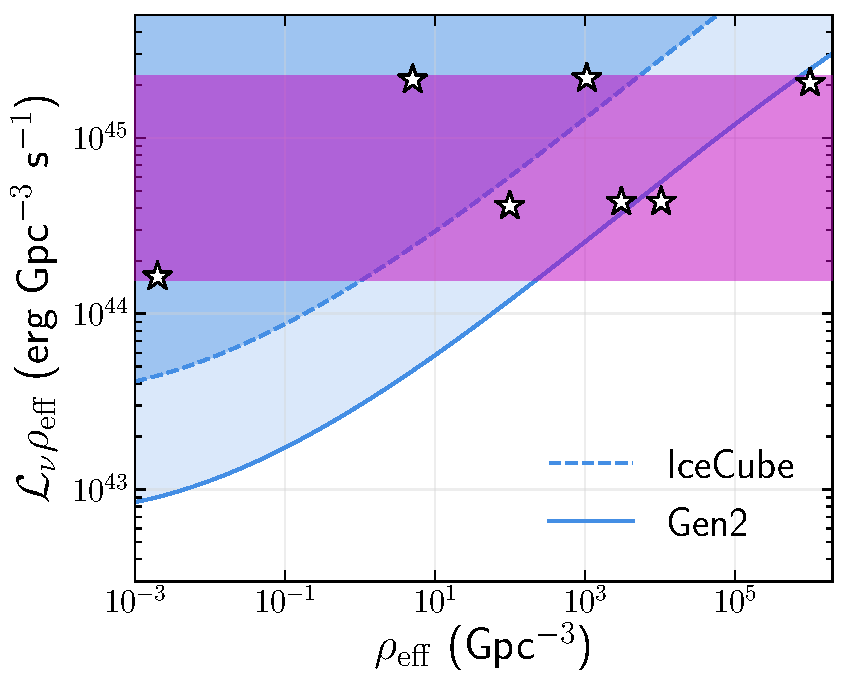
\includegraphics[width=0.48\textwidth]{figures/rotated_phase_space/lumi_density_product.pdf}
    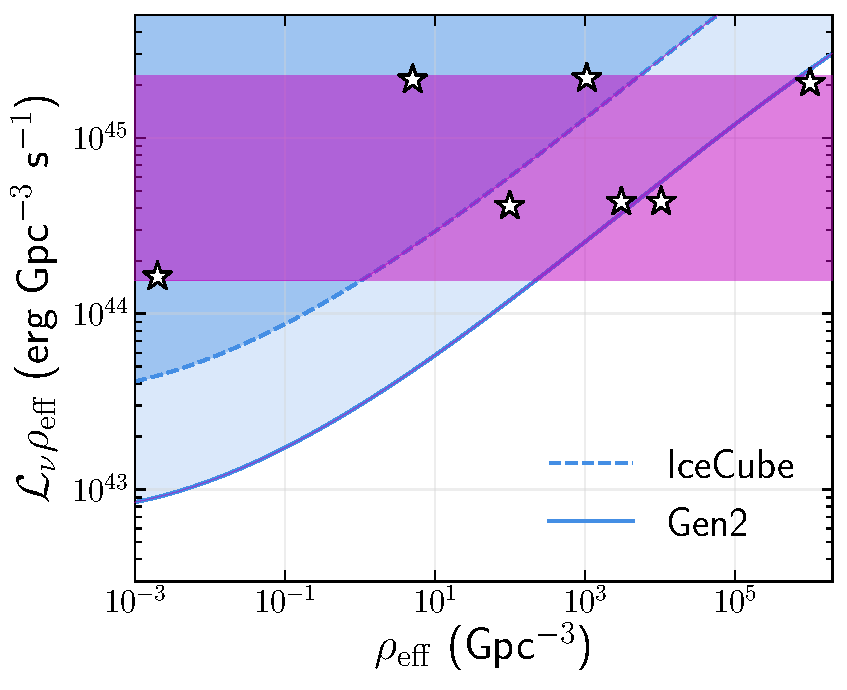
\includegraphics[width=0.48\textwidth]{figures/rotated_phase_space/lumi_density_product_hatch.pdf}
    \caption[Suggested visualization of luminosity-density parameter space]{Luminosity times effective local density plotted on the y-axis to focus on the interesting region of parameter space.}
    \label{fig:rotate_scaled_lumi_density}
\end{figure}

One nice consequence of this visualization is suppose you have a candidate source class that could produce a fraction, $f$ of the diffuse flux. Then (ignoring uncertainties on the diffuse flux), this just corresponds to moving down in the plot by a factor of $f$ from the vertical magenta line. This is shown in Figure~\ref{fig:rotate_diffuse_fraction_lumi}. 

\begin{figure}[h!]
    \centering
    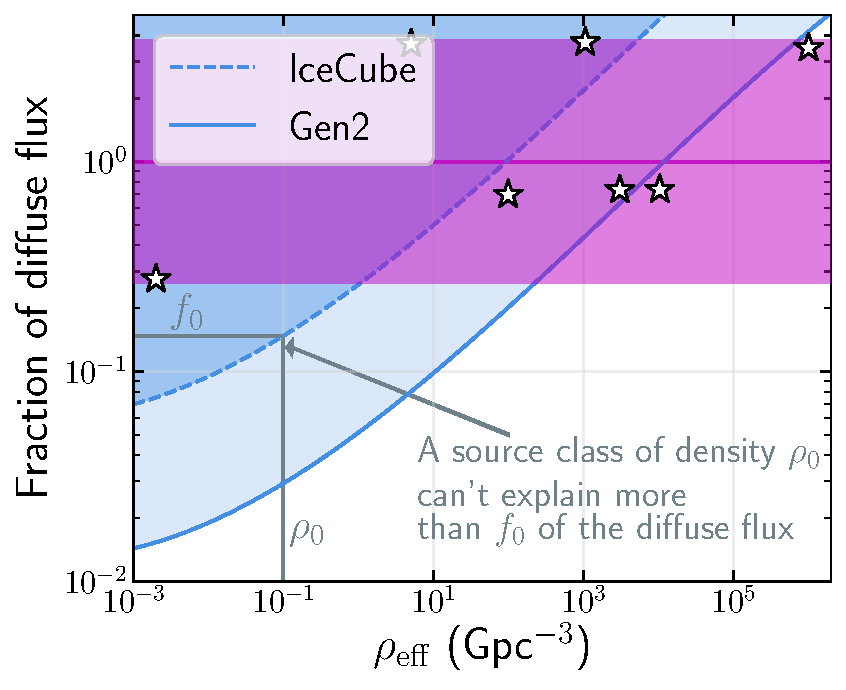
\includegraphics[width=0.5\textwidth]{figures/rotated_phase_space/lumi_density_fraction.pdf}
    \caption[Source number density phase space relative to diffuse flux]{Similar figure as above, scaled by the diffuse flux to highlight interpretation.}
    \label{fig:rotate_diffuse_fraction_lumi}
\end{figure}  %DONE
\chapter{Millipede Maps}
\label{sec:millipede}

\chapter{Effect of the geomagnetic field on cosmic-ray muons}
\label{sec:geomag_muons}
\chapter{ANITA Followup Paper}
\label{app:ANITA_collaboration_paper}

This and the following appendices contain papers to which I made significant contributions. The first, ``A search for IceCube events in the direction of ANITA neutrino candidates,'' corresponds to the analysis described in Chapter~\ref{sec:ANITA}. It set the first limits on astrophysical point source explanations of the ANITA events, and set constraining model-independent limits by leveraging the secondary \nutau distributions from \nutau regeneration. 

It was published in \textit{The Astrophysical Journal}, Volume 892, Number 1 on March 27, 2020. 

 %DONE
\chapter{ANITA \nutau regeneration paper}
\label{app:ANITA_few_author}

The paper attached in this section, ``Observing EeV neutrinos through the Earth: GZK and the anomalous ANITA events,'' outlines the software framework \texttt{TauRunner}\footnote{available at \url{https://github.com/IceCubeOpenSource/TauRunner}} and calculations surrounding \nutau regeneration from high-energy \nutau fluxes. 

The analysis has applications in constraining high-energy \nutau point-source fluxes as well as for searching for cosmogenic neutrinos. It was published in \textit{The Journal of Cosmology and Astroparticle Physics} on January 3, 2020 \citep{Safa:2019ege}.

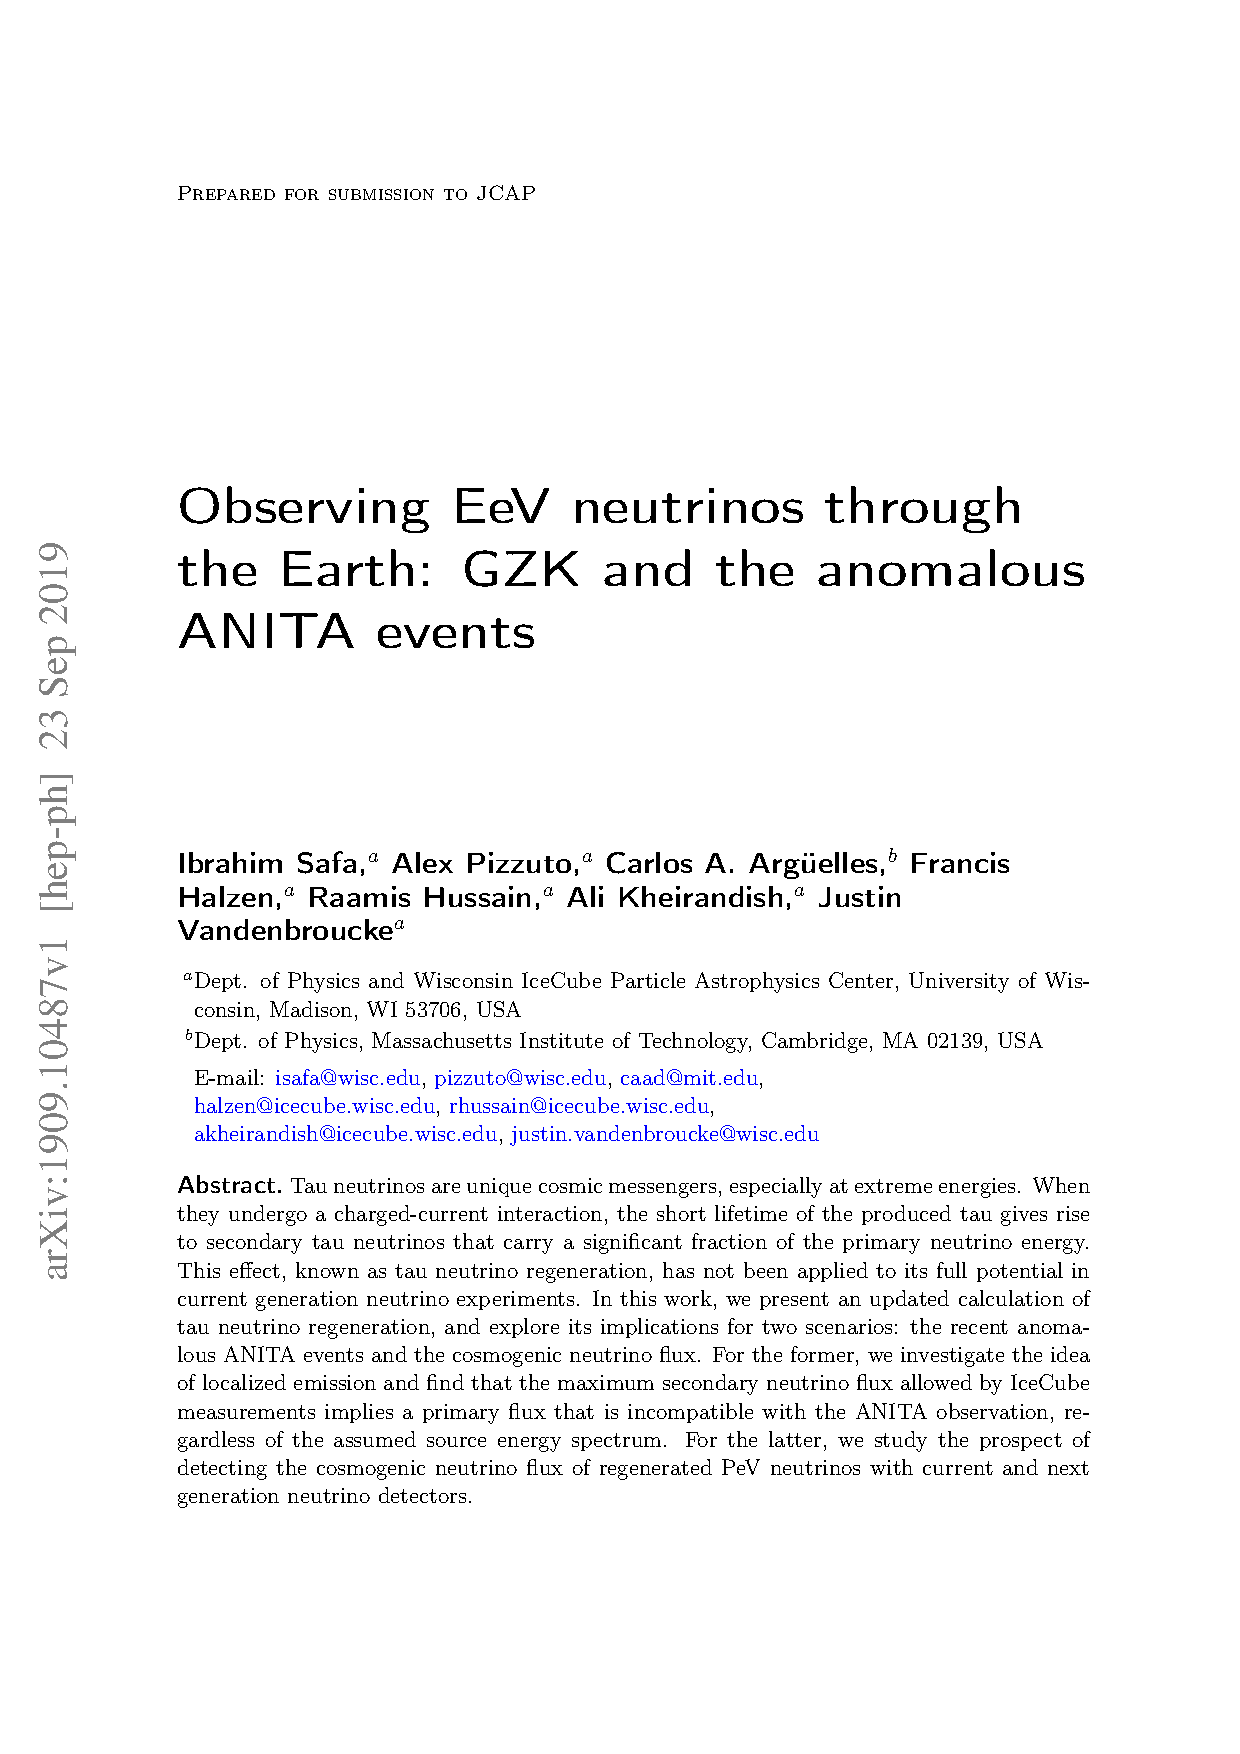
\includepdf[pages=-,pagecommand={},width=\pagewidth]{papers/ANITA_few_author_paper.pdf} %DONE
\chapter{Fast Response Analysis Paper}
\label{app:FRA_external_paper}

This appendix contains the paper which describes the Fast Response Analysis pipeline. The beginning of the paper serves as a technical explanation of the pipeline as well as a description of how we choose sources to follow up. It also summarizes the results from analyses which were run in response to external triggers (neglecting our followups of IceCube alert events). 

It was published in \textit{The Astrophysical Journal}, Volume XX, Number YY in BLABLABLA 2021.

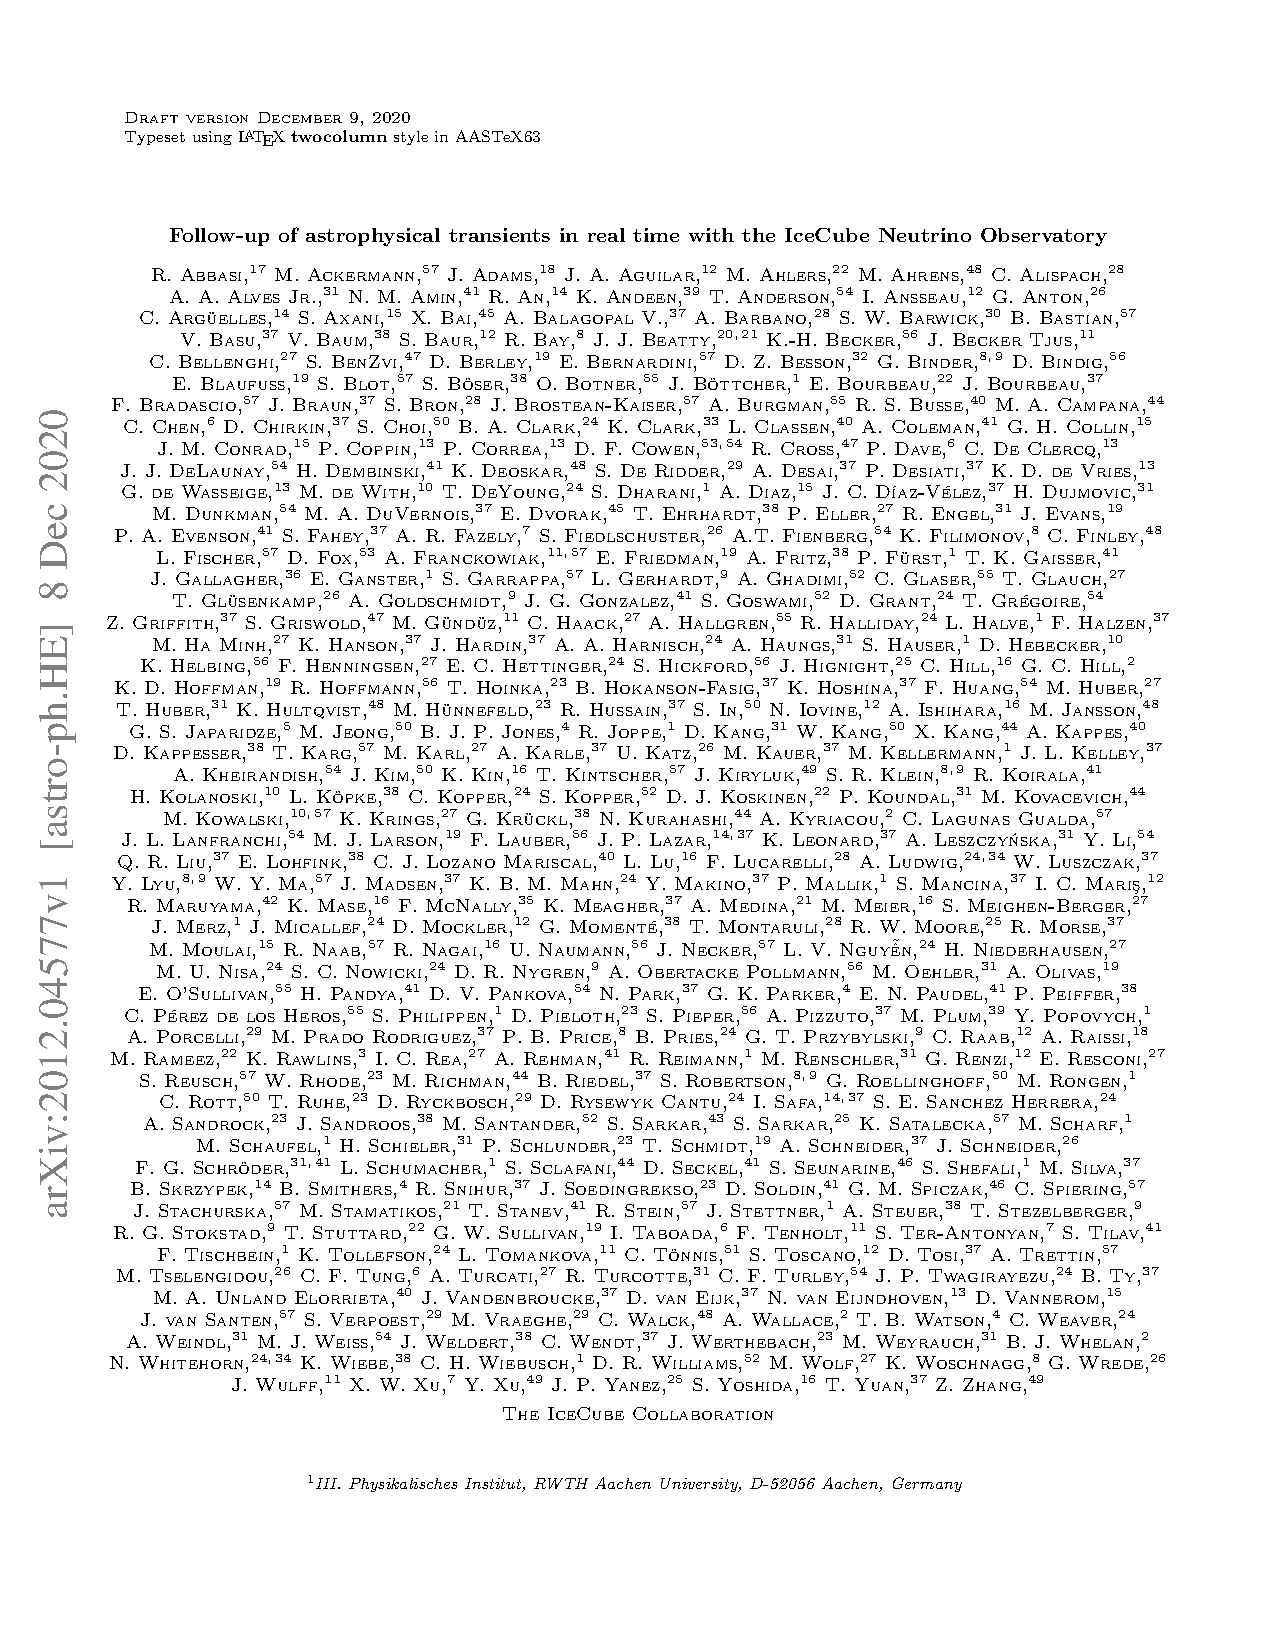
\includepdf[pages=-,pagecommand={},width=\pagewidth]{papers/FRA_external_paper.pdf}

 %DONE
\input{content/appendix-alert_followup_paper}
\input{content/appendix-nova_paper}
\input{content/appendix-DECO_monte_carlo_paper}
\nocite{*}
\clearpage

% --------------------------
% Back matter
% --------------------------
{%
\setstretch{1.1}
\renewcommand{\bibfont}{\normalfont\small}
\setlength{\biblabelsep}{0pt}
\setlength{\bibitemsep}{0.5\baselineskip plus 0.5\baselineskip}
%\bibliographystyle{abbrv}
\printbibliography
%\printbibliography[nottype=online]
%\printbibliography[heading=subbibliography,title={Websites},type=online,prefixnumbers={@}]
}
\clearpage

\listoffigures
\clearpage

\listoftables
\clearpage


% !TEX root = ../thesis-example.tex
%
%************************************************
% Declaration
%************************************************
\pdfbookmark[0]{Declaration}{Declaration}
\chapter*{Declaration}
\label{sec:declaration}
\thispagestyle{empty}

You can put your declaration here, to declare that you have completed your work solely and only with the help of the references you mentioned.

\bigskip

\noindent\textit{\thesisUniversityCity, \thesisDate}

\smallskip

\begin{flushright}
	\begin{minipage}{5cm}
		\rule{\textwidth}{1pt}
		\centering\thesisName
	\end{minipage}
\end{flushright}

%*****************************************
%*****************************************

\clearpage
\newpage
\mbox{}

% **************************************************
% End of Document CONTENT
% **************************************************
\end{document}
